\documentclass[
    BCOR=6mm,
    DIV=13,
    draft=false,
    titlepage=true,
    twoside=false,
    toc=bib,
    parskip=half-,
    chapterprefix=true,
    appendixprefix=true,
    footnotes=multiple,
    headsepline=true]{scrreprt}

% KOMA-Script related commands
\renewcommand*{\partformat}{\thepart\autodot}
\addtokomafont{disposition}{\rmfamily}
\setkomafont{paragraph}{\mdseries\itshape}
\RedeclareSectionCommand[beforeskip=-1sp,afterskip=1sp]{section}
\RedeclareSectionCommand[beforeskip=-1sp,afterskip=1sp]{subsection}
\RedeclareSectionCommand[beforeskip=-1sp,afterskip=1sp]{subsubsection}
\RedeclareSectionCommand[beforeskip=-1sp,afterskip=1sp]{paragraph}
\usepackage[automark,autooneside=false]{scrlayer-scrpage}
\lohead*{}
\cohead*{}
\rohead[]{\headmark}
\rofoot*{\pagemark}
\cofoot*{}
\lofoot*{}

% External packages and commands
%Packages
\usepackage[english]{babel}
\usepackage{lipsum}

% Conversion to PDF/1A
\usepackage[a-2b]{pdfx}
% Metadata -- does not get included in the pdf right now
\begin{filecontents}{main.xmpdata}
\Title{Elucidating the mechanism of AP axis alignment in the C. elegans embryo}
\Author{Bhatnagar, Archit}
\Copyright{Copyright \copyright\ 2023 "Bhatnagar, Archit"}
\Keywords{Anteroposterior axis\sep C. elegans\sep Pseudocleavage furrow\sep Actomyosin cortex\sep Active Matter}
\Subject{PhD Thesis submitted to TU Dresden Physics Faculty on the experimental work done to elucidate the biophysical mechanism behind the alignment of the Anteroposterior axis with the long axis in the ellipsoidal C. elegans embryo at the one-cell stage}
\end{filecontents}

% Hyperlinks
\usepackage{hyperref}
\hypersetup{
  colorlinks   = true, %Colours links instead of ugly boxes
  urlcolor     = black, %Colour for external hyperlinks
  linkcolor    = black, %Colour of internal links
  citecolor   = black %Colour of citations
}

%Images/Graphics packages
\usepackage{graphicx} 
\usepackage{verbatim} %Comments
\usepackage{xcolor}
\usepackage{xspace}
\usepackage{float}
\usepackage{placeins}

% Packages for tables
\usepackage{multirow}
\usepackage{array}
% New definitions of column types: see https://tex.stackexchange.com/questions/12703/how-to-create-fixed-width-table-columns-with-text-raggedright-centered-raggedlef
\newcolumntype{L}[1]{>{\raggedright\let\newline\\\arraybackslash\hspace{0pt}}m{#1}}
\newcolumntype{C}[1]{>{\centering\let\newline\\\arraybackslash\hspace{0pt}}m{#1}}
\newcolumntype{R}[1]{>{\raggedleft\let\newline\\\arraybackslash\hspace{0pt}}m{#1}}

% Package for subfigures -- allows setting figure layout in latex
\usepackage{caption}
\usepackage{subcaption}
\captionsetup{font=normalsize,labelfont={bf,sf},singlelinecheck=false}
\captionsetup[sub]{font=footnotesize,labelfont={bf,sf}}

% For formatting text justification
\usepackage{ragged2e}

% math packages
\usepackage{amsfonts,amssymb,amsbsy,amsmath,amsthm}
\usepackage{mathtools}

%Quotes
\usepackage[autostyle]{csquotes}

% Chemistry typesetting package
\usepackage[version=4]{mhchem}

%Math formatting packages
\usepackage{physics}

%Package for bibliography
\usepackage[
    natbib=true,
    style=numeric-comp,
    sorting=none]{biblatex}
\addbibresource{biblio.bib}

%Units definition - qty cannot be used
\usepackage{siunitx}
\sisetup{
    separate-uncertainty, % Value +- Error
    multi-part-units=single, % Single unit for both value and error, no brackets
    space-before-unit, % Unit spacing
    range-phrase=--, % Representing Ranges: L -- Ul
    range-units=single % Single unit for Ranges
}
\DeclareSIUnit{\unitAngle}{deg}
\DeclareSIUnit[per-mode=symbol]{\unitAngVel}{\unitAngle\per\second}
\DeclareSIUnit{\unitLength}{\micro\meter}
\DeclareSIUnit[per-mode=symbol]{\unitPostVel}{\unitLength\per\second}
\DeclareSIUnit[per-mode=symbol]{\unitCrtxVel}{\unitLength\per\minute}
\DeclareSIUnit{\hours}{hours}
\DeclareSIUnit{\unitRNAiTime}{\hours}
\DeclareSIUnit{\pixels}{pixel}
\DeclareSIUnit{\frames}{frame}
\DeclareSIUnit[per-mode=symbol]{\unitMyosinConc}{AU/pixel}

\DeclareSIUnit\molar{\mole\per\cubic\deci\metre}
\DeclareSIUnit\Molar{\textsc{m}}

% Acronyms
\usepackage[nohyperlinks]{acronym}
% Species names are not properly formatted, plus not sure if we want them in the abbreviations list anyway. Included here separately instead
\newacro{ce}[\textit{C. elegans}]{\textit{Caenorhabditis elegans}}
\newacro{ecoli}[\textit{E. coli}]{\textit{Escherichia coli}}

% New commands
\usepackage{ifthen}
\newcommand{\geneExp}[1]{\textit{#1}\xspace} % Typesetting RNAi and mutant (nop-1, dpy-11)
\newcommand{\flurophoreLabel}[2]{#1::#2} % For labels of fluorophores (ex: NMY-2::GFP)

% List of variables used throughout the thesis
\newcommand{\hydrodynamicLength}{$\lambda_H$\xspace}
\newcommand{\nematicLength}{$\lambda_N$\xspace}
\newcommand{\activeRelaxLength}{$\lambda_A$\xspace}
\newcommand{\dragCoefficient}{$d$\xspace}
\newcommand{\longAxisLength}{$a$\xspace}
\newcommand{\shortAxisLength}{$b$\xspace}
\newcommand{\aspectRatio}{$\flatfrac{a}{b}$\xspace}

% Commands for theory sections
% Introduction
\newcommand{\speciesSuper}[2]{#1^{(#2)}}
\newcommand{\inlinePartial}[3][1]{\ifthenelse{#1=1}{\partial_{#2} #3}{\partial^{#1}_{#2} #3}}
% Surface descriptions
\newcommand{\divSurf}{\mathrm{div}\:}
\newcommand{\gradSurf}{\mathrm{grad}\:}


\begin{document}
\pagenumbering{roman}

% Title-page (as per TUD requirements)
\begin{titlepage}
\vspace{1cm} 
\begin{center} 
    \Huge \textbf{Elucidating the mechanism of \acs{ap} axis alignment in the \acs{ce} embryo} \vspace{1cm}\\
    \Large \textbf{DISSERTATION \vspace{0.5cm}\\zur Erlangung des akademischen Grades \vspace{0.5cm}\\Doctor rerum naturalium \\(Dr. rer. nat.) \vspace{0.5cm}\\
    vorgelegt \vspace{0.5cm}\\dem Bereich Mathematik und Naturwissenschaften \\ der Technischen Universität Dresden\vspace{0.3cm} \\ von \vspace{0.3cm}\\
    B.Tech. Archit Bhatnagar \vspace{0.5cm}\\ geboren am 27.09.1996 in Jabalpur, India \vspace{0.5cm}\\ eingereicht am 28.03.2023\vspace{5mm}} \vspace{\fill}\\
    Die Dissertation wurde in der Zeit von September 2018 bis M{\"a}rz 2023 Max-Planck-Institut f{\"u}r molekulare Zellbiologie und Genetik angefertigt.
\end{center}
\clearpage
\thispagestyle{plain}
\hspace{\fill}{\huge To my parents and sister...}
\vspace*{\fill}
\end{titlepage}

\pagestyle{scrheadings}
%\chapterpagestyle{plain.scrheadings}
%\partpagestyle{plain.scrheadings}
%\automark[]{chapter}
%\automark*[]{section}

\addchap{Abbreviations}
\begin{acronym}
% AP axis alignment

% Introduction
\acro{ap}[AP]{Anteroposterior}
\acro{atp}[ATP]{Adenosine Tri-Phosphate}
\acro{mtoc}[MTOC]{Microtubule-organizing center}
\acro{nmy2}[NMY-2]{Non-Muscle myosin II}
\acro{rna}[RNA]{Ribonucleic acid}
\acro{rnai}[RNAi]{\acs{rna} mediated interference}
\acro{gfp}[GFP]{Green Fluorescent Protein}
\acro{par}[PAR]{Partitioning defective}
\acro{apar}[aPARs]{Anterior PAR proteins}
\acro{ppar}[pPARs]{Posterior PAR proteins}

% Methods
\acro{ngm}[NGM]{Nematode Growth Medium}
\acro{bf}[BF]{BrightField}
\acro{dsRNA}[dsRNA]{Double-stranded \acs{rna}}
\acro{fiji}[FIJI]{Fiji Is Just ImageJ}
\acro{piv}[PIV]{Particle Image Velocimetry}
\acro{matlab}[MATLAB]{MATrix LABoratory}
\acro{tub}[TUB]{Tubulin}

\end{acronym} %Add acronym definitions

\addchap{Abstract}
Development of a single-cell embryo into an adult multi-cellular organism features the establishment of upto three anatomical body axes - anteroposterior, dorsoventral and left-right. It has been observed in many organisms that these body axes can consistently orient relative with respect to the geometric features of the embryo in many organisms. One such example is observed in the model organism \acf{ce}, where the \acf{ap} axis coincides with the geometric long axis of the ellipsoidal embryo -- the shape being imposed by the surrounding eggshell. In \acs{ce}, the \acs{ap} axis is established at the one-cell stage via its polarization by \acs{par} polarity proteins. This cell polarization proceeds via a self-organized mechanochemical feedback between the \acs{par} proteins and mechanical flows in the actomyosin cortex, resulting in the formation of two mutually exclusive domains of \acl{apar} and \acl{ppar} proteins on the cortex denoting the future anterior and posterior end of the embryo -- and thus establishing the \acs{ap} axis. The initial orientation of the \acs{ap} axis is determined by the site of sperm entry at fertilization. However, the nascent \acs{ap} axis that forms after fertilization is observed to actively re-orient -- indicated by the movement of the \acs{par} domains and concurrent migration (here termed posteriorisation) of the sperm-donated male pronucleus -- such that it aligns with the long axis of the ellipsoidal embryo, if it is not already aligned. In effect, the site of sperm entry only determines which half of the embryo becomes the posterior half of the embryo. This phenomenon of active re-orientation of the \acs{ap} axis, that ensures that the \acs{ap} axis aligns with the long axis of the embryo, is termed \acs{ap} axis alignment. The work described in this thesis investigates the mechanism of this \acs{ap} axis alignment in the \acs{ce} embryo.

Anterior-directed flows in the actomyosin cortex observed during \acs{ap} axis establishment have also been found to be essential for \acs{ap} axis alignment. In this thesis, two possible mechanisms of \acs{ap} axis alignment are considered, both of which are consequences of these cortical flows. Cortical flows at the embryo surface can drive flows in the bulk cytoplasm in the embryo, generating cytoplasmic flows which point towards the sperm-donated male pronucleus as it posteriorises. Previous studies have proposed that these cytoplasmic flows could push onto the male pronucleus, and due to the ellipsoidal geometry of the embryo, drive it towards the closest tip of the embryo. This proposed mechanism is referred to as the cytoplasmic flow-dependent mechanism in this thesis. Another mechanism proposed in this thesis postulates that the reorientation of the \acs{ap} axis occurs via the repositioning of the pseudocleavage furrow. The pseudocleavage furrow is a contractile ring-like structure that forms at the boundary of the two \acs{par} domains during \acs{ap} axis establishment. The pseudocleavage furrow forms as a result of compressive alignment of actin filaments in the actomyosin cortex due to cortical flows. In cases where the \acs{ap} axis is not aligned with the long axis of the embryo, the pseudocleavage furrow is
not perpendicular to the long axis of the embryo. In such cases, active anisotropic stresses generated in the actomyosin cortex could force the rotation of the pseudocleavage furrow akin to an elastic rubber-band on an ellipsoid, and cause the \ac{ap} axis to re-orient towards the long axis of the embryo. This proposed mechanism is referred to as the pseudocleavage furrow-dependent mechanism in this thesis.

This thesis investigates the role played by the two mechanisms in \acs{ap} axis alignment. This is accomplished in the following way: a theoretical model of the \acs{ap} axis alignment is introduced, consisting of a description of the actomyosin cortex as an active nematic fluid present on the 2D surface of a fixed ellipsoid representing the embryo. This description of the cortex incorporates both the cytoplasmic flow-dependent mechanism and the pseudocleavage furrow-dependent mechanism. \acs{rnai} experiments in the \acs{ce} embryo that remove the pseudocleavage furrow, in conjuction with numerical simulations using the theoretical model, show that the pseudocleavage furrow-dependent mechanism is the predominant mechanism that drives \acs{ap} axis alignment, while cytoplasmic flow-dependent mechanism plays only a minor role. \acs{rnai} experiments that modify the geometry of the \acs{ce} embryo -- specifically, generate rounder embyros -- show that embryo geometry can influence the rate of re-orientation of the \acs{ap} axis during \acs{ap} axis alignment -- with slower \acs{ap} axis alignment in rounder embryos. Such an relation between embryo geometry and \acs{ap} axis alignment is found to be consistent with pseudocleavage furrow-dependent mechanism, both via predictions made using the theoretical model and using a simplified effective model of a contractile ring (or elastic rubber-band) on a fixed ellipsoid. 

Altogether, the work presented in this thesis shows \acs{ap} axis alignment observed in the \acs{ce} embryo is driven primarily by the anisotropic stresses in the actomyosin cortex that generate the pseudocleavage furrow. The work here also shows that the \acs{ap} axis alignment process is sensitive to the geometry of the embryo. In effect, active mechanical flows in the actomyosin cortex translate the ellipsoidal geometry of the embryo into a robust orientation of the \acs{ap} axis of the \acs{ce} embryo. Mechanical flows such as these are not exclusive to \acs{ce}, nor are specific orientations of the body axes with respect to the embryo geometry. The results in this thesis thus point towards a possibly general role of the interactions between mechanical flows and embryo geometry to properly orient the body axes of the developing embryos of many multi-cellular organisms.

\tableofcontents
\listoffigures

\cleardoubleoddpage
\pagenumbering{arabic}

\chapter{Introduction}\label{ch:APAxisIntro}
Development of a multi-cellular organism typically starts with a one-cell embryo. This one cell, generated as a result of fertilization (i.e. fusing of the male and female gametes), divides to give rise to the multiple cells and cell types that would eventually form the adult organism. A key question is how the correct arrangement of cells achieved. During development, upto three body axes: anterior-posterior (head-tail), dorsal-ventral (back-front) and left-right, are established. By patterning along these established body axes, proper arrangement of cells can be ensured during development \citep{goldstein1997axis}.

Thus, the body axes serve as the system of spatial axes that allow the embryo to specify position of cells. How are then these body axes established? For many organisms, the embryos start out with few initial asymmetries. Instead, external cues -- such as site of sperm (i.e. male gamete) entry, unequal cell division patterns, and gravity -- are utilized to break the symmetry in the embryo and initiate the establishment of body axes \citep{goldstein1997axis}. Mechanical forces coupled together with chemical patterns translate these external cues into an internal asymmetry of the embryo, by reorganizing certain determinants in the embryo \citep{goldstein1997axis,gross2017active}. As the embryo grows, this unequal distribution of determinants spans across the embryo, thus establishing a body axis \citep{meinhardt2015models,meinhardt2008models}.

It has been observed that the orientation of body axes is relatively fixed with respect to the geometric features of the embryo in many organisms (\autoref{fig:compareBodyAxesEmbryoGeometry}). For example, in many nematodes (roundworms; see \autoref{subfig:compareBodyAxesEmbryoGeometry-apAxisCelegans} for an example in \ac{ce}) the \acl{ap} axis is established at the one-cell stage, and forms along the long axis of the ellipsoidal embryo \citep{goldstein1997axis,goldstein1996specification}. In insect embryos such as fruit flies (see \autoref{subfig:compareBodyAxesEmbryoGeometry-apAxisDrosophila} for an example in \textit{Drosophila}), the \ac{ap} axis forms along the long axis of oocyte \citep{goldstein1997axis,dicko2017geometry,quinlan2016cytoplasmic,shulman2000drosophila,gonzalez1994role}. In chick embryos, Von Baer's rule indicates that the \ac{ap} axis typically forms perpendicular to the long axis of the egg \citep{goldstein1997axis,von1828entwicklungsgeschichte}, but this can be entrained by gravity \citep{kochav1971bilateral}. In mouse embryos (see \autoref{subfig:compareBodyAxesEmbryoGeometry-apAxisMouse}), the \ac{ap} axis initially forms along the axis of the cylindrically-shaped implanted embryo, but then is re-aligned to be along its short axis and transverse to its initial location \citep{tam2004embryonic,vianello2019understanding,hiramatsu2013external,matsuo2017mechanical}. 

\begin{figure}[p]

\centering
\begin{subfigure}{\textwidth}
    \centering
    \includegraphics[width=0.9\textwidth]{Introduction/FigureBodyAxesGeometry/celegans.pdf}
    \caption{\acs{ap} axis in \acs{ce} establishes along the long axis of the ellipsoidal embryo, with posterior half determined by site of sperm entry \citep{goldstein1996specification}. S denotes the sperm at fertilization; AB, P1, ABa, ABp, P2, EMS are names of subsequent blastomeres in embryogenesis (see \autoref{subsec:EarlyEmbryoCelegans} and \cite{strome1989generation}). Top: Sperm enters on the right, away from the female pronucleus -- leading to an embryo with anterior on the left and posterior on the right. Bottom: Sperm enters on the left -- leading to an embryo with anterior on the right and posterior on the left. DV indicates dorso-ventral axis. Adapted from \cite{goldstein1997axis}}
    \label{subfig:compareBodyAxesEmbryoGeometry-apAxisCelegans}
\end{subfigure}
\hfill
\begin{subfigure}{\textwidth}
    \centering
    \includegraphics[width=0.9\textwidth]{Introduction/FigureBodyAxesGeometry/drosophila.pdf}
    \caption{\acs{ap} axis in \textit{Drosophila} is established along the long axis during oogenesis, with posterior half determined by location of oocyte within the germline cyst \citep{gonzalez1994role}. Top: in the usual case, the oocyte migrates towards the posterior of the cyst, specifying the posterior follicle cells that help determine the posterior end. Bottom: if this migration does not occur, no \acs{ap} axis is established. Adapted from \cite{gonzalez1994role}}
    \label{subfig:compareBodyAxesEmbryoGeometry-apAxisDrosophila}
\end{subfigure}
\hfill
\begin{subfigure}{\textwidth}
    \centering
    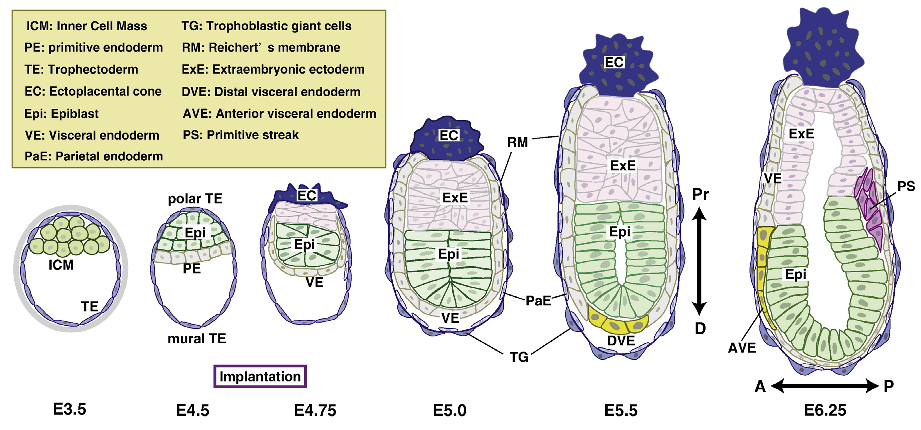
\includegraphics[width=0.9\textwidth]{Introduction/FigureBodyAxesGeometry/mouse.pdf}
    \caption{\acs{ap} axis in mouse is established during uterine implantation. Initial \acs{ap} axis forms along the long axis (Proximal-Distal) of the cylindrical embryo, indicated by the emergence of distal visceral endoderm (DVE) cells at E5.5. \acs{ap} axis reorients to the short axis as the DVE cells migrate to the lateral side, forming anterior visceral endoderm (AVE). Adapted from \cite{matsuo2017mechanical}}
    \label{subfig:compareBodyAxesEmbryoGeometry-apAxisMouse}
\end{subfigure}

\caption[Comparing orientation of \acs{ap} axis with geometry]{Comparing orientation of \acs{ap} axes with embryo geometry in different model organisms: \acs{ce}, \textit{Drosophila}, and mouse}
\label{fig:compareBodyAxesEmbryoGeometry}

\end{figure}

How does this orientation with respect to geometry achieved? Given that mechanical forces are involved in the establishment of body axes, could it be possible that the mechanical forces involved in body axes establishment play a role in achieving this relative orientation? Studies in the mouse embryo seem to suggest so \citep{vianello2019understanding,hiramatsu2013external,matsuo2017mechanical}, but how do mechanical forces enforce this relative orientation is not understood. In this thesis, this problem is studied in the the context of \ac{ap} axis establishment in the \ac{ce} embryo - a nematode. The aim of this thesis is to understand the mechanism(s) that ensure the alignment of the \ac{ap} axis of the \ac{ce} embryo along the long axis of the ellipsoidal embryo. 

In this chapter, the general features of the cytoskeleton in eukaryotic cells are first introduced. The actomyosin cortex, an important higher-order structure of cytoskeletonal elements present in almost all eukaryotic cells, is also described. Next, hydrodynamic theory of active matter is introduced -- the theoretical framework which will be used to model the actomyosin cortex in \autoref{ch:ActiveMatter}. Next, the model organism used in this thesis is introduced: \acl{ce}. The early development of \ac{ce} embryo is described, with focus on the establishment of \ac{ap} axis in the one-cell stage of the \ac{ce} embryo. Next, the phenomenon of \ac{ap} axis alignment -- the active reorientation of the \ac{ap} axis such that it aligns with the geometric long axis of the ellipsoidal embryo -- is described. Possible mechanisms of \ac{ap} axis alignment which have been suggested in previous studies, and explored in this thesis, are described. Finally, an overview of the thesis is provided -- encapsulating the work done in this thesis on elucidating the mechanism of \ac{ap} axis alignment in \ac{ce} embryo.

\section{Cytoskeleton}\label{sec:Cytoskeleton}
As noted above, mechanics plays an important role in the establishment of body axes. Cells thus need to react to the mechanics of their surrounding, and modify their own mechanical properties in response to different stimuli. The structure that allows cells to actively modify their mechanical properties, and perform mechanical tasks, is the cytoskeleton \citep{chaffey2003alberts,bray2001cell,fletcher2010cell}. It is essential in many cellular processes: maintaining cell shape \citep{chaffey2003alberts,rivero1996role,herrmann2007intermediate}, driving locomotion \citep{fletcher2010cell}, and cell division \citep{chaffey2003alberts,gonczy2001spindle}. Its role is to provide the cell with a dynamic mechanical scaffolding, allowing the cell to act as a highly adaptive mechanical entity to achieve different tasks \citep{chaffey2003alberts,bray2001cell,fletcher2010cell}.

The cytoskeleton is commonly defined as a network of protein filaments that extend throughout the cytoplasm of eukaryotic cells, although analogous filaments have also been identified in prokaryotes \citep{erickson2007evolution}. This meshwork of filaments is complemented by motor proteins that exert force betwen the filaments, crosslinking proteins that tie these filaments in the meshwork and various associated proteins that modify and remodel the meshwork \citep{chaffey2003alberts,bray2001cell,fletcher2010cell}. In this section, the elements that make up the cytoskeleton in the eukaryotic cells are introducted. Also introduced is the actomyosin cortex, a thin layer of cytoskeletonal elements present just below the cell membrane \citep{chaffey2003alberts,salbreux2012actin}, and the primary force-generating mechanical structure that this thesis focuses on.

\subsection{Main constituents of the cytoskeleton}\label{subsec:ComponentsCytoskeleton}
\subsubsection{Protein Filaments}\label{subsubsec:FilamentsCytoskeleton}
Protein filaments provide the backbone of the cytoskeleton. In eukaryotic cells, the cytoskeleton is composed of three principal types of protein filaments: actin filaments, intermediate filaments and microtubules. Monomeric protein subunits build each of these filaments. In contrast to usual polymers, these filaments are held together by non-covalent bonds, allowing fast assembly and disassembly \citep{chaffey2003alberts}. 

\paragraph{Actin filaments}
Actin filaments (or F-actin) are right-handed double helix composed of two protofilaments, each being a chain of actin monomers (or G-actin) \citep{pollard1986actin,pollard2000molecular} (see \autoref{subfig:cytoskeletonMainConsituents-actin}). Actin filaments are thin, with a typical diameter of around \SI{7}{\nano\meter} \citep{cooper2007cell}, and flexible, with a typical persistence length of \SI{17}{\micro\meter} \citep{ott1993measurement,gittes1993flexural}. The pitch of the helix formed by the protofilaments is typically around \SI{37}{\nano\meter}. Polymerisation of actin filaments is fueled by hydrolysis of \ac{atp} at the binding site on the monomers as they bind to the filament \citep{fujiwara2007polymerization}. Actin filaments are structurally polar, with a defined (+) or barbed end where new monomers preferentially bind, and a (-) or pointed end where monomers preferentially unbind \citep{pollard1986actin,pollard2000molecular,vavylonis2005actin}. Thus, actin filaments can undergo tread-milling, regulated by \ac{atp} \citep{wegner1982treadmilling}.

Actin filaments often gets organized into higher-order structure, such as the actomyosin cortex (described below), to perform various functions such as migration \citep{pollard2003cellular}, cell division \citep{sanger1975changing} and control of cell shape \citep{clarke1977nonmuscle}. 

\paragraph{Microtubules}
Microtubules are rigid hollow rod-like polymers, formed by the polymerization of a dimer of two globular proteins, $\alpha$-tubulin and $\beta$-tubulin \citep{chaffey2003alberts,nogales1998structure} (see \autoref{subfig:cytoskeletonMainConsituents-microtubule}). These dimers polymerize to form linear protofilaments that associate laterally to form the microtubule \citep{chaffey2003alberts}. Slight offset between protofilaments generates a pseudo-helical structure \citep{hunyadi2007microtubule}. The typical \enquote{\num{13}-\num{3}} arrangement, composed of \num{13} protofilaments with \num{3} dimer offset between neighbouring pairs, has a diameter of approximately \SI{25}{\nano\meter}, and a persistence length of approx \SI{5}{\milli\meter} \citep{chalfie1979organization,chaffey2003alberts,gittes1993flexural,ledbetter1963microtubule} -- practically rigid in most cells, given their typical sizes. Similar to actin filaments, microtubules are also polar, with a fast growing (+) end and a slow growing (-) end \citep{howard2003dynamics}. Microtubules serve various functions such as providing mechanical support, facilitating cell migration and locomotion \citep{mikhailov1998relationship}, acting as pathways for intracellular transport \citep{chaffey2003alberts}, and centering of the mitotic spindle \citep{pearson2004dynamic,grill2003distribution,grill2005theory}.

\textit{Centrosome}: Microtubules usually are nucleated at, and extend outwards from, a \ac{mtoc}, to which the (-) ends are attached. In animal cells, the major \ac{mtoc} is the centrosome, typically present near the nucleus when the cell is not dividing. At mitosis (i.e. when the cell is dividing), the centrosome duplicates \citep{chaffey2003alberts}. In most animal cells, a centrosome consists of a pair of cylinders (centrioles) surrounded by a meshwork of pericentriolar material \citep{pimenta2020pericentriolar}. Complexes of $\gamma$-tubulin in the centrosome serve as the nucleation sites for microtubule assembly \citep{kellogg1994centrosome}. In many animals, centrosomes play an important role in the formation of the mitotic spindle, an array of microtubules and associated proteins responsible for proper segregation of genetic material in the daughter cells after division \citep{bettencourt2013q,chaffey2003alberts}.

\paragraph{Intermediate filaments}
Different cell types also produce other filaments, with a typical diameter of \SI{10}{\nano\meter}. They typically play a structural role and provide mechanical support -- see \cite{chaffey2003alberts,herrmann2007intermediate} for a more detailed review.

\subsubsection{Motor proteins}\label{subsubsec:MotorCytoskeleton}
Motor proteins convert the chemical energy released in \ac{atp} hydrolysis into mechanical work \citep{chaffey2003alberts,bray2001cell,kolomeisky2007molecular,howard2002mechanics}. Motor proteins are categorized into three super-families, distinguished by the type of filaments they bind to. \textit{Myosins} are motors associated with actin filaments, while \textit{kinesins} and \textit{dyenins} bind to microtubules instead \citep{chaffey2003alberts}. Molecular motors perform various functions \citep{chaffey2003alberts}, such as cargo transport \citep{vale2003molecular} and serving as force generators for contraction of large-scale structures \citep{howard2002mechanics,carlsson2006contractile}.

Generally, motor proteins share a common set of \enquote{mechanical parts}: a track on which the motor walks (typically the protein filaments), some fuel (typically \ac{atp}), a transducer and force generator that converts the chemical energy of the fuel into a \enquote{power stroke} to generate mechanical force and a lever that transmits that force to the track \citep{hwang2009mechanical}. This is illustrated using the example of a particular myosin - \acs{nmy2}, which is a major component of the actomyosin cortex. 

\paragraph{\acl{nmy2}}
\ac{nmy2} is a member of the myosin super-family of motor proteins, and therefore a molecular motor that acts on actin filaments (see \autoref{subfig:cytoskeletonMainConsituents-myosin}). It is a major contractile protein of non-muscle eukaryotic cells \citep{chaffey2003alberts,holmes2008myosin}. \ac{nmy2} forms a hexamer consisting of three pairs of polypeptides: two heavy chains, two regulatory light chains involved in regulation of \ac{nmy2} activity and two essential light chains which stabilize the heavy chain conformation \citep{holmes2008myosin,vicente2009non}. Each heavy chain has a motor domain on one end (N-terminus) that binds to actin filament and \ac{atp}, followed by a neck domain to which the regulatory light chains bind, and a coiled-coil domain on the other end (C-terminus) that facilitates dimerization of the heavy chain \citep{holmes2008myosin,vicente2009non,robert2019force}. \ac{nmy2} usually organizes into myosin minifilaments, consists of around \num{28} \ac{nmy2} units \citep{holmes2008myosin,vicente2009non}. 

How does the \ac{nmy2} motor generate force? As depicted in \autoref{subfig:cytoskeletonMainConsituents-powerstroke}, when not bound to \ac{atp} myosin has a strong affinity to actin filament. \ac{atp} binding leads to dissociation of the motor domain from the actin filaments, and \ac{atp} hydrolysis ensues. During this step, the neck domain bends, allowing the motor domain to sample sites on the actin filaments. As myosin binds again to the filament, the products of \ac{atp} hydrolysis are released, resulting in the force generating step (that is, the power stroke) that displaces the motor along the filament with \SI{5}{\nano\meter} displacement, and returns it back to the initial state \citep{de2004relating,sweeney2010structural,tyska2002myosin,robert2019force}. Thus, the motor domains act as the transducer and force generators, the neck domain as the lever, the actin filament as the track and \ac{atp} as fuel for the \ac{nmy2} motor \citep{robert2019force,hwang2009mechanical}. \ac{nmy2} is a non-processive motor (it only makes one step before it detaches from the track \citep{howard2002mechanics,hwang2009mechanical}) with a low duty cycle (fraction of time spent bound to actin filament \citep{howard2002mechanics,hwang2009mechanical}) \citep{kovacs2003functional,wang2003kinetic}. Minifilaments of \ac{nmy2} can slide actin filaments past each other, by creating force dipoles \citep{vicente2009non,niederman1975human,mahajan1996assembly}. \ac{nmy2} also serves as an actin crosslinker \citep{xu2001during,mizuno2007nonequilibrium,laevsky2003cross}.

\begin{figure}[p]

\centering
\begin{subfigure}{\textwidth}
    \centering
    \includegraphics[width=0.9\textwidth]{Introduction/FigureCytoskeleton/actin.pdf}
    \caption{Sketch of an actin filament, red circles denote monomeric G-actin. Arrows indicate rate of chemical reaction at each end. Adapted from \cite{sebastian2012activeChiral}}
    \label{subfig:cytoskeletonMainConsituents-actin}
\end{subfigure}
\hfill
\begin{subfigure}{\textwidth}
    \centering
    \includegraphics[width=0.9\textwidth]{Introduction/FigureCytoskeleton/microtubules.pdf}
    \caption{Sketch of a \enquote{13-3} microtubule, composed of $\alpha$ and $\beta$ tubules. Arrows indicate rate of chemical reaction at each end. Adapted from \cite{sebastian2012activeChiral}}
    \label{subfig:cytoskeletonMainConsituents-microtubule}
\end{subfigure}
\hfill
\begin{subfigure}{\textwidth}
    \centering
    \includegraphics[width=0.9\textwidth]{Introduction/FigureCytoskeleton/myosin.pdf}
    \caption{Schematic of the forms of \acs{nmy2} motor protein. i) \acs{nmy2} converts from inactive state (left) to active state (right) via phosphorylation. Active state has three domains: the globular head containing the motor and actin binding domains, the neck domain or lever arm, and a long coiled-coil domain of heavy chains. ii) \acs{nmy2} can assemble into bipolar filaments -- myosin minifilaments -- and can slide antiparallel actin filaments past each other. Adapted from \cite{vicente2009non}}
    \label{subfig:cytoskeletonMainConsituents-myosin}
\end{subfigure}
\hfill
\begin{subfigure}{\textwidth}
    \centering
    \includegraphics[width=0.85\textwidth]{Introduction/FigureCytoskeleton/powerstroke.pdf}
    \caption{Schematic of the power stroke of \acs{nmy2}. Refer to text for details on power stroke. Adapted from \cite{de2004relating}}
    \label{subfig:cytoskeletonMainConsituents-powerstroke}
\end{subfigure}

\caption[Main constituents of the cytoskeleton]{Main constituents of the cytoskeleton in eukaryotic cells}
\label{fig:cytoskeletonMainConsituents}

\end{figure}

\subsubsection{Associated proteins}\label{subsubsec:AssociatedProteinsCytoskeleton}
Most of the known cytoskeletal proteins are neither filamentenous nor motors. Instead, they modify and interact with the existing protein filaments and motors, to dynamically alter the mechanical properties of the cytoskeleton. A comprehensive overview of the these proteins and their functions is presented in \cite{chaffey2003alberts,pollard1986actin}; here only a brief review of some of the important functions these proteins fulfill is presented.

\textit{Nucleators} help initiate the formation of protein filaments, by providing a nucleation point. \textit{Capping proteins} bind to the ends of filaments, blocking polymerisation at the end where they bind. These proteins thus can either stabilise or de-stabilise a protein filament, depending on where they bind. \textit{Severing proteins} cut filaments. \textit{Crosslinkers} and \textit{bundling proteins} organize protein filaments into structured networks, and modify them. \textit{Sequestering proteins} help with recycling unbound monomers, while \textit{Sidebinding proteins} act as molecular rulers. \textit{Linkers} link filaments of different kinds, allowing different filaments (such as the microtubules and actin filaments) to influence each other. \textit{Regulators} regulate the action of other proteins. Note that individual proteins can have multiple functions, and thus belong to multiple categories.

\subsection{Actomyosin cortex}\label{subsec:ActomyosinCortex}

\begin{figure}[h]
    \centering
    \includegraphics[width=\textwidth]{Introduction/FigureActomyosin/actomyosinSketch.pdf}
    \caption[Sketch of actomyosin cortex]{Sketch of the actomyosin cortex as a quasi-2D polymeric meshwork of actin filaments below the cell membrane (composed of lipids) and interspersed with myosin motors and other proteins. Top represents an effective 2D representation of the actomyosin cortex that could be obtained by averaging over the thickness of the cortex. Adapted from \cite{kumar2021actomyosin}}
    \label{fig:actomyosinCortexSketch}
\end{figure}

The actomyosin cortex, also called the cell cortex, is a thin (around few hundred nanometers \citep{clark2013monitoring}) polymeric meshwork of cross-linked actin filaments, interspersed with myosin motors and associated proteins, that lies just below the cell membrane of most eukaryotic cells \citep{bray1988cortical,chaffey2003alberts} (see \autoref{fig:actomyosinCortexSketch}). Analysis using cryo-electron tomography and atomic force microscopy revealed that actin filaments organize in both isotropic meshworks and actin bundles \citep{hartwig1991cytoskeleton,heuser1980filament,morone2006three,medalia2002macromolecular,pesen2005micromechanical}. 

The cortex is not, however, a static structure -- \ac{atp} hydrolysis fuels the polymerization and de-polymerization of actin filaments, activity of the associated proteins, and force generation by myosin motors. This external energy input and resultant active remodeling of the cortex drives it far from equilibrium, and makes it a very dynamic structure. This highly cross-linked and dynamic nature of the cortex makes it behave like a viscoelastic material \citep{kumar2021actomyosin,salbreux2012actin}, as confirmed by laser ablation experiments \citep{saha2016determining,mayer2010anisotropies}. In live cells, the active remodeling in the cortex occurs on timescales of around \SI{30}{\second} \citep{fritzsche2016actin}, and elastic stresses relax on comparable timescales \citep{saha2016determining}. As a consequence, the cortex can effectively be considered as a viscous fluid on longer timescales. Force generation by myosin motors confer the cortex with a tendency to actively contract \citep{carlsson2006contractile} -- the actomyosin cortex can thus be considered as active viscous fluid.

Actomyosin cortex helps the cell to adapt to changing environmental conditions by controlling cell mechanics. The cortex determines the stiffness of the cell surface, and opposes osmotic pressure \citep{stewart2011hydrostatic}. Global increase in contractility of the cortex facilitates the rounding of the cell before its division \citep{kunda2008moesin}. Local changes in cortex contractility can create gradients of cortical tension. Such changes can aid in cell migration, via retraction of the rear of the cell from the substrate \citep{vicente2009non}. Developmental processes at the tissue scale can also be directed by the cortex of the constituent cells \citep{rauzi2011cortical} -- such as dorsal closure in \textit{Drosophila} \citep{martin2010pulsation} and convergence extension in \textit{Xenopus} \citep{zhou2009actomyosin}. \autoref{sec:ApAxisEstablishment} discusses how local changes in contractility in the one-cell stage \ac{ce} embryo drive flows in the actomyosin cortex of the \ac{ce} embryo, and what role these cortical flows play in the \ac{ap} axis establishment of \ac{ce} \citep{mayer2010anisotropies}.

\section{Hydrodynamic theory of active fluids}\label{sec:introHydrodynamicTheoryActiveFluids}
As discussed in the previous section, the actomyosin cortex can and has been modelled as an active viscous fluid in many previous studies \citep{kumar2021actomyosin,salbreux2012actin,bois2011pattern,saha2016determining,mayer2010anisotropies,fritzsche2016actin,julicher2018hydrodynamic}. General physical principles that govern the behaviour of active biological materials such as the actomyosin cortex can be identified using a hydrodynamic approach \citep{de2013non,julicher2018hydrodynamic,bois2011pattern,gross2017active,reymann2016cortical,kruse2004Asters,salbreux2012actin,julicher2022surface,Kruse2005GenericTO,Prost2015ActiveGP}. By its generic nature, such an approach is not unique to the actomyosin cortex, and has been used to describe other active materials such as bird flocks \citep{toner1995long,toner1998flocks,tu1998sound}, swarms of hydrodynamically interacting swimmers \citep{simha2002hydrodynamic,hatwalne2004rheology}, active polar gels \citep{Prost2015ActiveGP,kruse2004Asters,Kruse2005GenericTO,elgeti2011defect,julicher2018hydrodynamic,julicher2022surface}, active nematic fluids \citep{marenduzzo2007hydrodynamics,fielding2011nonlinear,giomi2011excitable,julicher2018hydrodynamic,julicher2022surface} and active solids \citep{gunther2007spontaneous,banerjee2011instabilities,ranft2010fluidization,julicher2018hydrodynamic}. While the microscopic mechanisms at play in these different active materials can differ considerably, in the hydrodynamic limit -- that is, on large length and long time-scales compared to the microscopic mechanisms of the active material at hand -- general properties of active materials are described by a general hydrodynamic theory corresponding to conservation laws and broken continuous symmetries in the material \citep{julicher2018hydrodynamic,julicher2022surface,Kruse2005GenericTO,Prost2015ActiveGP,de2013non}. In such a theory, a small set of phenomenological coefficients capture the details of the microscopic mechanisms at play in the particular active material under consideration.

This section reviews the general hydrodynamic theory of active fluids based on irreversible thermodynamics. This hydrodynamic theory is a generalization of the hydrodynamics and statistical mechanics of liquid crystals \citep{de1993physics} to systems maintained away from thermodynamic equilibrium by chemical processes driven by fuel(s) provided in external reservoir(s). In the context of the actomyosin cortex, \ac{atp} may serve the role of such a chemical fuel -- utilized by myosin motors to generate mechanical forces in the cortex. Hydrodynamic equations that govern the properties of active fluids can be obtained systematically, by first identifying the conjugate pairs of thermodynamic fluxes and forces. Constitutive material relations can then be expressed via a linear coupling between the thermodynamic fluxes and forces, respecting the Onsager reciprocity relation \citep{onsager1931reciprocalI,onsager1931reciprocalII,mazur1953onsager,casimir1945onsager} and Curie symmetry principle \citep{curie1894symmetry} Phenomenological constants that capture various microscopic processes appear in these constitutive relations. This section closely follows the description presented in \cite{julicher2018hydrodynamic,de2013non,sebastian2012activeChiral}.

At a microscopic level, any active fluid is made up of a large number $N$ of discrete molecules, each with individual mass, position and velocity. A description of the fluid in microscopic details requires that all of the $6N$ degrees of freedoms be tracked, which is infeasible for any active fluid given the large number of molecules involved. Instead, a coarse-grained description of the active fluid is utilized -- in which the fluid is divided into a large number of small volume elements, each of volume $V$. Using this description, densities of molecular components, momentum and energy can be defined for each volume element. To obtain a continuous description of these densities, the continuum limit is considered. Under this limit, the volume $V \rightarrow 0$, with the understanding that the volume still remains large compared to the molecular length scales of the fluid at hand. It is assumed that this continuum limit can always be considered. Altogether, this allows the properties of the active fluid to be described by continuous functions: such as mass density $\rho = \rho(\vec{r})$, flow velocity $\vec{v} = \vec{v}(\vec{r})$ etc. (where $\vec{r}$ is the position vector). The aim of the general hydrodynamic theory reviewed here is to derive dynamic equations for these continuous functions representing the local properties of the active fluid.

Note that Einstein summation is used throughout this section -- summation over repeated indices is implied. Greek alphabet indices assume values $x,y,z$ -- corresponding to the three spatial axes.

\subsection{Conservation Laws}\label{subsec:conservationLaws}
Mass, momentum, angular momentum and energy are conserved quantities, at all scales -- microscopic or macroscopic. This also remains valid in active fluids. Thus, local conservation laws, expressed in terms of the coarsed-grained properties of the active fluid, can be written. 

\subsubsection{Mass conservation}\label{subsubsec:massConserve}
Consider a fixed volume $V$ within the fluid, with boundary $\Omega$, with mass density (mass per unit volume) $\rho$ and flow velocity $\vec{v}$ at any given position $\vec{r}$. Then, the flux of mass flowing out of this fluid is given by:
\begin{equation*}
    \textrm{Mass flux outwards} = \int_{\Omega} \rho \vec{v}\cdot\dd{\vec{\Omega}}
\end{equation*}
However, since mass is conserved within this volume, this flux must match the change in total mass of the volume of fluid. Thus,
\begin{equation*}
    \int_{\Omega} \rho \vec{v}\cdot\dd{\vec{\Omega}} = - \dv{t}\int_V \rho \dd{V} = - \int_V \pdv{\rho}{t} \dd{V}
\end{equation*}
where $t$ is time. The exchange of derivative and integral is allowed since $V$ is fixed. Note that this is true for any arbitrary volume $V$ -- however small or big. Thus, using Gauss' theorem, the following continuity equation can be written:
\begin{equation}\label{eq:introMassBalance}
    \inlinePartial{t}{\rho} + \inlinePartial{\alpha}{\left(\rho v_\alpha\right)} = 0
\end{equation}
The mass flux -- that is, momentum density -- is thus given by $g_\alpha = \rho v_\alpha$

\subsubsection{Energy conservation}\label{subsubsec:energyConserve}
Similar to mass density, an energy density $e$ can be defined for the active fluid. Energy conservation implies that $e$ obeys the following continuity equation:
\begin{equation}\label{eq:introEnergyBalance}
    \inlinePartial{t}{e} + \inlinePartial{\alpha}{\speciesSuper{J}{e}_\alpha} = 0
\end{equation}
where $\speciesSuper{\vec{J}}{e}$ is the energy flux. This flux term can be split into two parts: a convective flux $e\vec{v}$ and a relative flux $\speciesSuper{\vec{j}}{e}$:
\begin{equation}\label{eq:introEnergyFlux}
    \speciesSuper{J}{e}_\alpha = ev_\alpha + \speciesSuper{j}{e}_\alpha
\end{equation}
This relative flux $\speciesSuper{\vec{j}}{e}$ describes the flux of energy in a co-moving reference frame with respect to the volume element at the given position in the fluid. Thus, this relative flux denotes the intrinsic changes in energy density at a given position in the fluid, separate from the changes in energy density caused due to exchange with surrounding volume elements.

\subsubsection{Momentum and Angular Momentum conservation}\label{subsubsec:momentumConserve}
As noted earlier, the momentum density is given by $g_\alpha = \rho v_\alpha$. Momemtum conservation then requires that the following continuity equation is obeyed:
\begin{equation}\label{eq:introMomentumBalance}
    \inlinePartial{t}{g_\alpha} + \inlinePartial{\beta}{\left(g_\alpha v_\beta\right)} = \inlinePartial{\beta}{\sigma_{\alpha\beta}}
\end{equation}
Here, the momentum flux due to convection is $g_\alpha v_\beta$. The total change in momentum of any volume element must match the forces applied onto it on its surface -- which is given by the stress $\sigma_{\alpha\beta}$. Using Gauss' theorem leads to \autoref{eq:introMomentumBalance}.

Similar continuity equations for angular momentum can also be considered -- as presented in \cite{julicher2018hydrodynamic,sebastian2012activeChiral}. However, note that for a non-trivial continuity equation for angular momentum, there must be intrinsic (or spin) angular momentum in the active fluid under consideration. For simplicity, it is assumed that the active fluid under consideration does not have any such intrinsic angular momentum -- both in this section and in \autoref{ch:ActiveMatter}. Thus, angular momentum is conserved, and consequently stress $\sigma_{\alpha\beta}$ is symmetric.

Also, using \autoref{eq:introMassBalance} and \autoref{eq:introMomentumBalance} along with $g_\alpha = \rho v_\alpha$ yields:
\begin{equation}\label{eq:introMomentumBalanceVelocityForm}
    \rho\left(\inlinePartial{t}{v_\alpha} + v_\beta\inlinePartial{\beta}{v_\alpha}\right) = \inlinePartial{\beta}{\sigma_{\alpha\beta}}
\end{equation}

\subsubsection{Particle number conservation}\label{subsubsec:speciesBalance}
The general case of a multi-species active fluid consisting of $N+1$ different species of particles is first considered. In this fluid, the particle number density (number of particles per unit volume) for species $i$ is denoted as $\speciesSuper{n}{i}$, with $i = 0,\ldots,N$. Using the same method as above, the continuity equation for $\speciesSuper{n}{i}$ can be written as:
\begin{equation}\label{eq:introSpeciesBalance}
    \inlinePartial{t}{\speciesSuper{n}{i}} + \inlinePartial{\alpha}{\speciesSuper{J}{i}_\alpha} = \speciesSuper{r}{i}
\end{equation}
where $\speciesSuper{\vec{J}}{i}$ is the flux of particles of species $i$, and $\speciesSuper{r}{i}$ the reaction rate accounting for all the chemical reactions in which species $i$ participates. Note that the number of particles of species $i$ is not conserved in the presence of chemical reactions (that is, a non-zero $\speciesSuper{r}{i}$).

The flux term $\speciesSuper{\vec{J}}{i}_\alpha$ can be split into a convective flux $\speciesSuper{n}{i}v_\alpha$ and a relative flux $\speciesSuper{\vec{j}}{i}$:
\begin{equation}\label{eq:introRelativeSpeciesFlux}
    \speciesSuper{J}{i}_\alpha = \speciesSuper{n}{i}v_\alpha + \speciesSuper{j}{i}_\alpha
\end{equation}
This relative flux $\speciesSuper{\vec{j}}{i}$ describes the movements of species $i$ relative to the volume element at the given position in the fluid -- and thus relative to the local flow of the fluid. Since the mass density can expressed in terms of $\speciesSuper{n}{i}$ as $\rho = \sum_{i=0}^N \speciesSuper{m}{i} \speciesSuper{n}{i}$ (where $\speciesSuper{m}{i}$ is the mass of each particle of species $i$), mass conservation \autoref{eq:introMassBalance} and particle number conservation \autoref{eq:introSpeciesBalance} dictate that:
\begin{equation*}
    \sum_{i=0}^N \speciesSuper{m}{i} \speciesSuper{j}{i}_\alpha = 0, \quad \textrm{and} \quad \sum_{i=0}^N \speciesSuper{m}{i} \speciesSuper{r}{i} = 0
\end{equation*}
with the latter of the two corresponding to the Laviosier's principle of mass conservation in chemical reactions. Using these, the relative flux and reactive rate for one species can be expressed in terms of those for other species. Choosing $i = 0$ yields $\speciesSuper{j}{0}_\alpha = -\frac{1}{\speciesSuper{m}{0}}\sum_{i=1}^N\speciesSuper{m}{i}\speciesSuper{j}{i}_\alpha$ and $\speciesSuper{r}{0} = -\frac{1}{\speciesSuper{m}{0}}\sum_{i=1}^N\speciesSuper{m}{i}\speciesSuper{r}{i}$. Thus, $\speciesSuper{\vec{j}}{0}$ and $\speciesSuper{r}{0}$ can be eliminated. For $M$ linearly independent chemical reactions, additional $M$ relations between the species -- based on the chemical reactions under considerations -- can also be derived. Thus, for an active fluid with $N+1$ species involved in $M$ reactions, $N - M$ independent conservation laws can be obtained for the species number densities $\speciesSuper{n}{i}$. Note that none of the species $i = 0,\ldots,N$ are part of fuel(s) in the external reservoir. For any such fuel species, the above considerations may not apply due to the reservoir. 

For the rest of this discussion, a simpler version of active fluids is assumed -- a three component fluid with the fluid particles, fuel molecules and their reaction products. Furthermore, it is assumed that the concentrations of the fuel and reaction products in the fluid are kept constant via contact with the external reservoir, thus implying $\speciesSuper{\vec{j}}{i} = 0$. The fluid is then kept out of equilibrium by consumption of the chemical fuel at a fixed reaction rate $r$. In the context of the actomyosin cortex, this scenario represents the simplest description of consumption of \ac{atp} (as fuel) by myosin motors -- with the local reaction rate $r$ of \ac{atp} hydrolysis proportional to the local myosin concentration.

\subsection{Continuously broken symmetries}\label{subsec:introLocalOrder}

\begin{figure}
\centering
\begin{subfigure}{0.25\textwidth}
    \centering
    \includegraphics[width=\textwidth]{Introduction/FigureLocalOrdering/isotropic.pdf}
    \caption{Isotropic ordering.\\$\norm{\vec{p}} = 0;\quad \norm{\vec{n}} = 0$}
    \label{subfig:introTheoryLocalOrdering-isotropic}
\end{subfigure}
\hfill
\begin{subfigure}{0.25\textwidth}
    \centering
    \includegraphics[width=\textwidth]{Introduction/FigureLocalOrdering/polar.pdf}
    \caption{Polar ordering.\\$\norm{\vec{p}} = 1;\quad \norm{\vec{n}} = 1$}
    \label{subfig:introTheoryLocalOrdering-polar}
\end{subfigure}
\hfill
\begin{subfigure}{0.25\textwidth}
    \centering
    \includegraphics[width=\textwidth]{Introduction/FigureLocalOrdering/nematic.pdf}
    \caption{Nematic ordering.\\$\norm{\vec{p}} = 0;\quad \norm{\vec{n}} = 1$}
    \label{subfig:introTheoryLocalOrdering-nematic}
\end{subfigure}
\caption[Continuous broken symmetries in complex fluids]{Continuous broken symmetries in complex fluids. The arrows represent the microscopic orientation $\vec{a}$ of the particles that constitute the fluid. The system is in isotropic state in \autoref{subfig:introTheoryLocalOrdering-isotropic} due to the random orientation of $\vec{a}$, in a polar state in \autoref{subfig:introTheoryLocalOrdering-polar} due to the orientation vectors $\vec{a}$ being aligned and parallel and in a nematic state in \autoref{subfig:introTheoryLocalOrdering-nematic} due to the orientation vectors $\vec{a}$ being aligned but anti-parallel.}
\label{fig:introTheoryLocalOrdering}
\end{figure}

In complex active fluids, the constituent molecules can be anisotropic. Many active fluids in biological systems are complex fluids -- such as the actomyosin cortex, in which the actin filaments are structurally polar (see \autoref{subsec:ComponentsCytoskeleton}). Arrangement or bundling of these actin filaments can further break local symmetry -- creating polar or nematic order throughout the fluid. 

In the context of the hydrodynamic theory discussed here, this effect can be captured by endowing each of the constituent particles of the active fluid with an orientation unit vector $\vec{a}$. Note that these orientation vector are a property of each particle -- and is thus not a coarse-grained variable that can be directly used in the hydrodynamic theory. Instead, coarse-grained variables can be derived by inspecting the local distribution of these orientation vectors in a volume element at the position of interest. If all the moments of the local distribution of $\vec{a}$ (that is, within the volume element) vanish, the fluid is isotropic -- and thus does not possess any local order. This is the case for all simple fluid, and with many active fluids. Consequently, locally ordered fluids have non-vanishing moments. 

If the first moment of the local distribution of $\vec{a}$ is non-zero, the fluid has a polar order. For each volume element, a polarity vector $\vec{p}$ can be then defined as the first moment:
\begin{equation}\label{eq:introPolarityVectorDefine}
    \vec{p}(\vec{r}) = \expval{\vec{a}}_{\textrm{Volume element at }\vec{r}}
\end{equation}
where the average is taken in the volume element at the position $\vec{r}$. Under the continuum limit, the polarity vector is a continuous vector function defined at each position and is the coarse-grained order parameter that characterises the local polar order in the active fluid. At any given position, the polarity vector has magnitude of \num{1} if the underlying orientation vectors in the volume element are perfectly aligned and parallel. The polarity vector is $\vec{0}$ for an isotropic fluid, or if the orientation vectors are aligned but anti-parallel. 

If the second moment of the local distribution of $\vec{a}$ is non-zero, the fluid has a nematic order. For each volume element, a nematic tensor $Q_{\alpha\beta}$ can be then defined as the second moment:
\begin{equation}\label{eq:introNematicTensorDefine}
    Q_{\alpha\beta}(\vec{r}) = \expval{a_\alpha a_\beta - \frac{1}{3} \delta_{\alpha \beta}}_{\textrm{Volume element at }\vec{r}}
\end{equation}
where the average is taken in the volume element at the position $\vec{r}$, and the nematic tensor is written for a fluid in 3-dimensions. Under the continuum limit, the nematic tensor $Q_{\alpha\beta}$ is a continuous function defined at each position and is the coarse-grained order parameter that characterises local nematic order in the active fluid. Note that in \autoref{eq:introNematicTensorDefine}, $\vec{a} \rightarrow -\vec{a}$ does not change the nematic tensor $Q_{\alpha\beta}$ -- indicating that the nematic tensor $Q_{\alpha\beta}$ is a measure of the alignment of orientation vectors, but not if those vectors are parallel. Specifically, this implies that the case of orientation vectors being aligned but anti-parallel has a nematic order, but not a polar order. As before, the nematic tensor is zero for an isotropic fluid. 

From the definition in \autoref{eq:introNematicTensorDefine}, one may note that $Q_{\alpha\beta}$ is symmetric ($Q_{\alpha\beta} = Q_{\beta\alpha}$) and traceless ($Q_{\gamma\gamma} = \expval{a_\gamma a_\gamma - \frac{1}{3} \delta_{\gamma \gamma}} = \expval{1 - \frac{3}{3}} = 0$). In the case of uniaxial nematic ordering where $Q_{\alpha\beta}$ has two equal eigenvalues, $Q_{\alpha\beta}$ may instead be written as:
\begin{equation}\label{eq:introNematicTensorUniaxialDefine}
    Q_{\alpha\beta} = S\left(n_\alpha n_\beta - \frac{1}{3}\delta_{\alpha\beta}\right)
\end{equation}
where the unit vector $\vec{n}$ is the nematic director and scalar $S \in [-\flatfrac{1}{2},1]$ corresponds to the degree of alignment of the orientation vectors along the nematic director $\vec{n}$. The nematic director is an eigenvector of the third non-equal eigenvalue of $Q_{\alpha\beta}$. The nematic order of the active fluid may equivalently be represented using the nematic director field. For the isotropic case, $S = 0$; while for the fully aligned case, $S = 1$.

Higher order moments of the local distribution of $\vec{a}$ are usually ignored. In the discussion that follows and in \autoref{ch:ActiveMatter}, the focus is on the nematic tensor $Q_{\alpha\beta}$ and therefore active nematic fluids. Note that as the actomyosin cortex may be considered as an active nematic 2-dimensional fluid on the cell membrane \citep{kumar2021actomyosin,julicher2022surface} (see \autoref{ch:ActiveMatter}). In 2-dimension, only a uniaxial nematic ordering is possible -- as $Q_{\alpha\beta}$ cannot have more than 1 independent eigenvalue.

\subsection{Irreversible thermodynamics of active fluids}\label{subsec:introIrrevThermoActiveFluids}
\subsubsection{Entropy production}\label{subsubsec:introEntropyProduction}
To be able to apply thermodynamic principles to derive the hydrodynamic theory for active fluids, a key assumption of local equilibrium is made. Specifically, it is assumed that each of the volume elements that comprise the active fluid are individually in thermodynamic equilibrium, but out of equilibrium with their neighbours. In this case, the active fluid is locally at equilibrium, but is globally maintained away from equilibrium. Such a local equilibrium can be considered if the small volume elements equilibriate at short times compared to the slow hydrodynamics time scales at large scales. 

Consider now only a single volume element (with volume $V$) at a position $\vec{r}$. Its \enquote{macroscopic} state -- as the volume element is still large enough to contain a large number of constituent particles of the fluid -- is then defined by the various coarse-grained variables defined before, such as: mass density $\rho$, internal energy $e$ and nematic tensor $Q_{\alpha\beta}$ for the active nematic fluid. Under the local equilibrium, one may then define the free energy $F = fV$ and entropy $S = sV$ of this volume element as a function of these coarse-grained variables. Equivalently, for the active fluid, free energy density (free energy per unit volume) $f$ and entropy density (entropy per unit volume) $s$ can be defined. Due to local equilibrium at each volume element, both $s = -\pdv{f}{T}$ and $f = e - Ts$ are valid -- where $T$ is the temperature of the local volume element. Here, only the isothermal case is considered: thus $T$ is the temperature of the whole fluid. Note that the whole fluid is not at equilibrium, in contrast to the locally equilibriated volume elements. However, the fluid's free energy and entropy are well-defined as a sum of local contributions of the locally equilibriated volume elements, and can be expressed in terms of free energy density $f$ and entropy density $s$ as:
\begin{equation}\label{eq:introFreeEnergyEntropyDensityDefine}
    F = \int f \dd{V}; \quad S = \int s \dd{V}
\end{equation}
where the integration is performed over the whole fluid.
 
Consider now the change in the total entropy of the fluid. The change in entropy may be written as a sum of two terms:
\begin{equation}\label{eq:entropyExtrinsicIntrinsic}
    \dd{S} = \dd_{\textrm{e}}S + \dd_{\textrm{i}}S
\end{equation}
where $\dd_{\textrm{e}}S$ is the entropy supplied to the fluid by its surroundings (and thus extrinsic to the fluid), and $\dd_{\textrm{i}}S$ is the entropy produced inside the fluid (and thus intrinsic to the fluid). The second law of thermodynamics states that the irreversible processes in a non-equilibrium system, such as the active fluid, lead to intrinsic production of entropy, implying:
\begin{equation*}
    \dd_{\textrm{i}}S \geq 0
\end{equation*}
with equality only for an equilibrium system. The entropy supplied however can be positive, negative or zero -- depending on the interaction of the fluid with its surroundings. Defining the flux of entropy as $\speciesSuper{\vec{J}}{S}$, and the entropy production rate per unit volume as $\theta$, \autoref{eq:entropyExtrinsicIntrinsic} can be transformed into a continuity equation for the local entropy density $s$:
\begin{equation}\label{eq:introEntropyBalance}
    \inlinePartial{t}{s} + \inlinePartial{\alpha}{\speciesSuper{J}{S}_\alpha} = \theta
\end{equation}
where $\theta > 0$ to satisfy the second law of thermodynamics. Note that $\dd_e S = -\inlinePartial{\alpha}{\speciesSuper{J}{S}_\alpha}$ -- the entropy supplied to the local volume element is related to the entropy flux entering the local volume element. Such a transformation is only possible because of assumption of local equilibrium -- without this assumption, a local entropy density $s$ and entropy production per unit volume $\theta$ do not make sense.

Using \autoref{eq:introEnergyBalance} and \autoref{eq:introEntropyBalance}, along with $f = e - Ts$, one may then write a continuity equation for the free energy density $f$:
\begin{equation}\label{eq:introFreeEnergyBalance}
    \inlinePartial{t}{f} = \inlinePartial{t}{e} - T\inlinePartial{t}{s} = -\inlinePartial{\alpha}{\speciesSuper{J}{e}_\alpha - T\speciesSuper{J}{s}_\alpha} -T\theta \implies \inlinePartial{t}{f} + \inlinePartial{\alpha}{\speciesSuper{J}{f}_\alpha} = -T\theta 
\end{equation}
where $\speciesSuper{\vec{J}}{f} = \speciesSuper{\vec{J}}{e} - T\speciesSuper{\vec{J}}{s}$ is identified as the flux of free energy. Thus, the rate of change of the free energy of the fluid $F = \int f \dd{V}$ for a fixed volume $\mathcal{V}$ of fluid is given by:
\begin{equation}\label{eq:introTotalFreeEnergyTimeDerivativeEntropyProduction}
    \dv{F}{t} = \int_{\mathcal{V}} (-T\theta) \dd{V} + \int_{\partial \mathcal{V}} \speciesSuper{\vec{J}}{f}\cdot\dd{\vec{\Omega}}
\end{equation}
The surface integral term can be interpreted as the work done on the fluid at its surface.

Another way to obtain the rate of change of the free energy of the fluid would be to specify the free energy density $f$. Given the assumption of local equilibrium for each volume element, the free energy per unit volume of the volume element in a co-moving frame can be written. Let this relative free energy density be denoted as $f_0 = f_0(Q_{\alpha\beta},\inlinePartial{\gamma}{Q_{\alpha\beta}})$, which depends on the local nematic tensor and its gradients for the 
active nematic fluid. Then,
\begin{equation}\label{eq:introTotalFreeEnergyDirect}
    f = \frac{g_\alpha g_\alpha}{2\rho} + f_0(Q_{\alpha\beta},\inlinePartial{\gamma}{Q_{\alpha\beta}}); \quad F = \int_{\mathcal{V}} \dd{V} \left(\frac{g_\alpha g_\alpha}{2\rho} + f_0(Q_{\alpha\beta},\inlinePartial{\gamma}{Q_{\alpha\beta}})\right)
\end{equation}
The rate of change of the free energy can then be obtained directly from \autoref{eq:introTotalFreeEnergyDirect}. Comparing the bulk term of the time derivative of free energy thus obtained to \autoref{eq:introTotalFreeEnergyTimeDerivativeEntropyProduction} then yields the entropy production rate per unit volume $\theta$.

\subsubsection{Linear Response theory}\label{subsubsec:introLinearResponse}
In general, the rate of entropy production can be expressed as a sum of products of generalized thermodynamics forces $F_n$ and their conjugate thermodynamic fluxes $J_n$:
\begin{equation}\label{eq:introEntropyProductionGeneral}
    T\theta = \sum_n J_nF_n
\end{equation}
where index $n$ specifies a thermodynamic variable or a tensor/vector component of a given variable. Summation over such an index are explicitly noted here (and thus do not follow the Einstein convention). Equivalently, $J_n$ and $F_n$ can be identified from the expression of rate of entropy production derived previously, using \autoref{eq:introEntropyProductionGeneral}. Note that at equilibrium, all $J_n$ and $F_n$ vanish -- leading to $\theta = 0$, as expected for a system at equilibrium.

Close to equilibrium, the thermodynamic fluxes $J_n$ can be expressed as linear functions of the thermodynamic forces $F_n$:
\begin{equation}\label{eq:introLinearExpansion}
    J_n = \sum_m L_{nm}F_m
\end{equation}
and thus, 
\begin{equation}
    T\theta = \sum_m L_{nm}F_nF_m
\end{equation}
where $L_{nm}$ are Onsager coefficients that capture the active fluid's material properties. Note that $L_{nm}$ themselves can be scalars, vectors or tensors, as is the case with $J_n$ and $F_n$. \autoref{eq:introLinearExpansion} gives the constitutive equations of the material. The second law of thermodynamics requires that $\theta > 0$ for systems not in equilibrium, for all values of the thermodynamic forces $F_n$. Thus, the matrix $L_{nm}$ must be positive definite for the active fluid. This leads to:
\begin{equation}
    L_{nn} > 0; \quad L_{nn}L_{mm} \geq \frac{1}{4}(L_{nm} + L_{mn})^2
\end{equation}
for the diagonal elements $L_{nn}$ and off-diagonal elements $L_{nm}, L_{mn}$.

\subsubsection{Curie symmetry principle}\label{subsubsec:introCurieSymmetry}
In principle, \autoref{eq:introLinearExpansion} allows for any thermodynamic flux $J_n$ to be expressed as a linear function of all thermodynamic forces $F_n$. However, all the fluxes $J_n$ and $F_n$ do not possess the same tensorial character, not do they possess the same symmetry properties. The expansion of a thermodynamic flux $J_n$ into thermodynamic forces $F_n$ must respect the symmetry properties and tensorial character of the flux $J_n$ -- this is the Curie symmetry principle. This principle restricts the choices of $L_{nm}$. For example, in isotropic systems, the Curie principle can be used to show that fluxes and forces of different tensorial ranks do not couple \citep{de2013non}.

\subsubsection{Onsager reciprocity relations}\label{subsubsec:introOnsager}
Another restriction on $L_{nm}$ arises from the Onsager reciprocity relations. These relations arise as a result of invariance under time reversal of microscopic mechanisms. For these relations, the signature $\epsilon$ of the thermodynamic fluxes $J_n$ and forces $F_n$ under time reversal must first be specified. Note that since entropy production $\theta$ has the signature $\epsilon(\theta) = -1$, the signatures of force $F_n$ is opposite to that of its conjugate flux $J_n$: $\epsilon(F_n) = -\epsilon(J_n)$, as a consequence of \autoref{eq:introEntropyProductionGeneral}. From \autoref{eq:introLinearExpansion}, a coefficient $L_{nm}$ couples a flux $J_n$ to a force $F_m$. Thus, the coefficients $L_{nm}$ can be classified based on the signature of the corresponding thermodynamic fluxes and forces they couple: $L_{nm}$ is a reactive coupling if $\epsilon{J_n} = \epsilon(F_m)$, and dissipative if $\epsilon{J_n} = -\epsilon(F_m)$. Reactive coupling are denoted as $L^r_{nm}$, dissipative coupling as $L^d_{nm}$. Then, Onsager reciprocity relations state that:
\begin{subequations}\label{eq:OnsagerRelations}
    \begin{align}
        L^r_{nm} &= -L^r_{mn}\\
        L^d_{nm} &= L^d_{mn}
    \end{align}
\end{subequations}
Note that, by the definition of reactive and dissipative coupling, coupling between a force and its conjugate flux is always dissipative: $L_{nn} = L^d_{nn}$. Essentially, the Onsager relations allow decomposition of the Onsager coefficient matrix $L_{nm}$ into a symmetric dissipative part $L^d_{nm}$ and an antisymmetric reactive part $L^r_{nm}$.

\subsubsection{Hydrodynamics of an active isotropic fluid}\label{subsubsec:introExampleSimpleIsotropicFluid}
The above concepts may be illustrated with an example of an active isotropic fluid. The free energy density of such a fluid is given by $f = \frac{g_\alpha g_\alpha}{2\rho} + f_0$, where $f_0$ is dependent on the fuel that drives this fluid out of equilibrium. Here, the fluid is considered to be under pressure $p$. Then, \autoref{eq:introTotalFreeEnergyDirect} can be written as:
\begin{equation}\label{eq:introActiveSimpleFluidFreeEnergyTotal}
    F = \int \dd{V} \left[\frac{g_\alpha g_\alpha}{2\rho} + f_0\right] - (\textrm{Work done by pressure})
\end{equation}
Note that $f_0$ is a volume term, since the fuel reaction happens in all volume elements. 

As an example, let the activity in this fluid be driven by hydrolysis of \ac{atp} into ADP and $\textrm{P}_\textrm{i}$:
\begin{equation*}
    \textrm{ATP} \rightarrow \textrm{ADP} + \textrm{P}_\textrm{i}
\end{equation*}
Note that this reaction happens at all locations in the fluid. Let $\mu_{\textrm{ATP}}$, $\mu_{\textrm{ADP}}$, $\mu_{\textrm{P}}$ be the chemical potentials for \ac{atp}, ADP and $\textrm{P}_\textrm{i}$ respectively. The change in free energy density in the co-moving frame $f_0$ then can be written as:
\begin{equation}\label{eq:introSimpleActiveFluidFreeEnergyDensityRelative}
    \delta f_0 = \mu_{\textrm{ATP}}\delta c_{\textrm{ATP}} + \mu_{\textrm{ADP}}\delta c_{\textrm{ADP}} + \mu_{\textrm{P}}\delta c_{\textrm{P}}
\end{equation}
where $c_{\textrm{ATP}}$, $c_{\textrm{ADP}}$, $c_{\textrm{P}}$ are the concentrations of \ac{atp}, ADP and $\textrm{P}_\textrm{i}$ respectively. Matter conservation for the chemical reaction above requires that:
\begin{equation}
    \delta c_{\textrm{ATP}} + \delta c_{\textrm{ADP}} = 0; \quad \delta c_{\textrm{ATP}} + \delta c_{\textrm{P}} = 0
\end{equation}
Thus, the rate of change in $f_0$ may be written as:
\begin{equation}\label{eq:introSimpleActiveFluidFreeEnergyDensityRelativeRate}
    \delta f_0 = (\mu_{\textrm{ATP}} - \mu_{\textrm{ADP}} - \mu_{\textrm{P}})\delta c_{\textrm{ATP}} = \Delta\mu\delta c_{\textrm{ATP}} \implies \dv{f_0}{t} = \Delta\mu\dv{c_{\textrm{ATP}}}{t} = - r\Delta\mu
\end{equation}
where $\Delta\mu$ is the difference in chemical potential for the \ac{atp} hydrolysis reaction, and $r = -\dv{c_{\textrm{ATP}}}{t}$ is the rate of consumption of \ac{atp} and thus the reaction rate of \ac{atp} hydrolysis.

Returning to \autoref{eq:introActiveSimpleFluidFreeEnergyTotal}, the rate of work done by pressure (opposing change in volume of each volume element) is given by $p\inlinePartial{\alpha}{v_\alpha} \dd{V}$. From this and \autoref{eq:introSimpleActiveFluidFreeEnergyDensityRelativeRate}, the rate of change of free energy of the fluid can be derived:
\begin{align*}
    \dv{F}{t} &= \int \dd{V} \left[\pdv{t}\left(\frac{g_\alpha g_\alpha}{2\rho}\right) - r\Delta\mu - p\inlinePartial{\alpha}{v_\alpha}\right] = \int \dd{V} \left[\frac{g_\alpha}{\rho}\inlinePartial{t}{g_\alpha} - \frac{g_\alpha g_\alpha}{2\rho^2}\inlinePartial{t}{\rho} - r\Delta\mu - p\inlinePartial{\alpha}{v_\alpha}\right]\\
    &= \int \dd{V} \left[v_\alpha\left(\inlinePartial{\beta}{\sigma_{\alpha\beta}} - \inlinePartial{\beta}{(g_\alpha v_\beta)}\right) + \frac{v_\alpha v_\alpha}{2}\inlinePartial{\beta}{g_\beta} - p\inlinePartial{\alpha}{v_\alpha}  - r\Delta\mu\right]\\
    &= \int \dd{V} \left[v_\alpha\inlinePartial{\beta}{\sigma_{\alpha\beta}} - \left(v_\alpha\inlinePartial{\beta}{(g_\alpha v_\beta)} - \frac{v_\alpha v_\alpha}{2}\inlinePartial{\beta}{g_\beta}\right) - p\inlinePartial{\alpha}{v_\alpha}  - r\Delta\mu\right]
\end{align*}
where \autoref{eq:introMassBalance} and \autoref{eq:introMomentumBalance} have been used, and $g_\alpha = \rho v_\alpha$. Now,
\begin{align*}
    &\frac{v_\alpha v_\alpha}{2}\inlinePartial{\beta}{g_\beta} = \frac{1}{2}\inlinePartial{\beta}{(\rho v_\alpha v_\alpha v_\beta)} - \rho v_\beta v_\alpha \inlinePartial{\beta}{v_\alpha}\\
    &v_\alpha\inlinePartial{\beta}{(g_\alpha v_\beta)} = \inlinePartial{\beta}{(\rho v_\alpha v_\alpha v_\beta)} - \rho v_\alpha v_\beta \inlinePartial{\beta}{v_\alpha}\\
    &\implies v_\alpha\inlinePartial{\beta}{(g_\alpha v_\beta)} - \frac{v_\alpha v_\alpha}{2}\inlinePartial{\beta}{g_\beta} = \frac{1}{2}\inlinePartial{\beta}{(\rho v_\alpha v_\alpha v_\beta)}\\
    &v_\alpha\inlinePartial{\beta}{\sigma_{\alpha\beta}} = \inlinePartial{\beta}{v_\alpha\sigma_{\alpha\beta}} - \sigma_{\alpha\beta}\inlinePartial{\beta}{v_\alpha}
\end{align*}
Using these, the rate of change of free energy is given by:
\begin{equation}\label{eq:introActiveSimpleFluidFreeEnergyRate}
    \dv{F}{t} = \int -\left[\sigma_{\alpha\beta}\inlinePartial{\beta}{v_\alpha} + p\inlinePartial{\alpha}{v_\alpha} - r\Delta\mu\right] \dd{V} + \int \dd{V} \inlinePartial{\beta}{\left[\frac{\rho v_\alpha v_\alpha v_\beta}{2} + v_\alpha \sigma_{\alpha\beta}\right]}
\end{equation}
Comparing to \autoref{eq:introTotalFreeEnergyTimeDerivativeEntropyProduction}, the entropy production rate can be written as:
\begin{equation}\label{eq:introActiveSimpleFluidEntropyProduction}
    T\theta = \sigma_{\alpha\beta}\inlinePartial{\beta}{v_\alpha} + p\inlinePartial{\alpha}{v_\alpha} + r\Delta\mu
\end{equation}

Note that the entropy production is not in the form required by \autoref{eq:introEntropyProductionGeneral} (since at equilibrium neither $\sigma_{\alpha\beta}$ nor $p$ vanish). To do so, the stress tensor $\sigma_{\alpha\beta}$ and velocity gradient $\inlinePartial{\beta}{v_\alpha}$ are decomposed. For $\sigma_{\alpha\beta}$:
\begin{equation*}
    \sigma_{\alpha\beta} = \left[\sigma_{\alpha\beta} - \frac{1}{d}\sigma_{\gamma\gamma}\delta_{\alpha\beta}\right] + \left[\frac{1}{d}\sigma_{\gamma\gamma} + p\right]\delta_{\alpha\beta} - p\delta_{\alpha\beta} = \Tilde{\sigma}^{d,s}_{\alpha\beta} + \sigma^d\delta_{\alpha\beta} -p\delta_{\alpha\beta}
\end{equation*}
where $\Tilde{\sigma}^{d,s}_{\alpha\beta} = \sigma_{\alpha\beta} - \frac{1}{d}\sigma_{\gamma\gamma}\delta_{\alpha\beta}$ is the symmetric traceless part of $\sigma_{\alpha\beta}$, $\sigma^d = \frac{1}{d}\sigma_{\gamma\gamma} + p$ is isotropic part of the stress $\sigma_{\alpha\beta}$ and $d$ is the number of space dimensions. Note that the notation followed here is borrowed from \cite{julicher2018hydrodynamic}. The superscript $d$ refers to the deviatoric part of the stress -- that is, the stress tensor excess from the equilibrium stress. Since for the isotropic fluid, the equilibrium stress tensor is just $-p\delta_{\alpha\beta}$, the above definitions are obtained. For $\inlinePartial{\beta}{v_\alpha}$:
\begin{equation*}
    \inlinePartial{\beta}{v_\alpha} = \left[\frac{\inlinePartial{\beta}{v_\alpha} + \inlinePartial{\alpha}{v_\beta}}{2} - \frac{1}{d}\inlinePartial{\gamma}v_\gamma\delta_{\alpha\beta}\right] + \frac{\inlinePartial{\beta}{v_\alpha} - \inlinePartial{\alpha}{v_\beta}}{2} + \frac{1}{d}\inlinePartial{\gamma}v_\gamma\delta_{\alpha\beta} = \Tilde{v}_{\alpha\beta} + \omega_{\alpha\beta} + \frac{1}{d}\inlinePartial{\gamma}v_\gamma\delta_{\alpha\beta}
\end{equation*}
where $\Tilde{v}_{\alpha\beta} = \frac{\inlinePartial{\beta}{v_\alpha} + \inlinePartial{\alpha}{v_\beta}}{2} - \frac{1}{d}\inlinePartial{\gamma}v_\gamma\delta_{\alpha\beta}$ is the symmetric traceless part of $\inlinePartial{\beta}{v_\alpha}$, $\omega_{\alpha\beta} = \frac{\inlinePartial{\beta}{v_\alpha} - \inlinePartial{\alpha}{v_\beta}}{2}$ is the antisymmetric part of $\inlinePartial{\beta}{v_\alpha}$ and $\frac{1}{d}\inlinePartial{\gamma}v_\gamma$ is the local expansion rate of the fluid. Rewriting \autoref{eq:introActiveSimpleFluidEntropyProduction}:
\begin{equation}\label{eq:introActiveSimpleFluidEntropyProductionOnsager}
    T\theta = \Tilde{\sigma}^{d,s}_{\alpha\beta}\Tilde{v}_{\alpha\beta} + \sigma^d\inlinePartial{\gamma}v_\gamma + r\Delta\mu
\end{equation}
Note that each of $\Tilde{\sigma}^{d,s}$, $\sigma^d$ and $\Delta \mu$ go to zero at equilibrium -- first two because the stress at equilibrium is just $-p\delta_{\alpha\beta}$ and $\Delta \mu$ since at equilibrium the chemical potential difference would be zero (indicating that the hydrolysis reaction does not have preferred direction). Thus, \autoref{eq:introActiveSimpleFluidEntropyProductionOnsager} is in the form of \autoref{eq:introEntropyProductionGeneral}.

Using \autoref{eq:introActiveSimpleFluidEntropyProductionOnsager}, the thermodynamic fluxes and forces can be identified. In here, the choice of forces and fluxes is made are shown in \autoref{tab:introActiveSimpleFluidFluxesForces}. Note that the choice of fluxes and forces is arbitrary -- a force may be treated as a flux and vice versa. Only the pairs themselves are determined by \autoref{eq:introActiveSimpleFluidEntropyProductionOnsager}.
\begin{table}[h]
    \centering
    \begin{tabular}{|c|c|c|c|}
        \hline
        Flux $J_n$ & Force $F_n$ & Time reversal signature $\epsilon(J_n), \epsilon(F_n)$ & Rotation symmetry\\
        \hline
        $\Tilde{\sigma}^{d,s}_{\alpha\beta}$ & $\Tilde{v}_{\alpha\beta}$ & 1,-1 & Traceless symmetric tensor\\
        $\sigma^d$ & $\inlinePartial{\gamma}v_\gamma$ & 1,-1 & Scalar \\
        $r$ & $\Delta \mu$ & -1,1 & Scalar \\
        \hline
    \end{tabular}
    \caption{Conjugate thermodynamic fluxes and forces for a simple isotropic fluid}
    \label{tab:introActiveSimpleFluidFluxesForces}
\end{table}

Using \autoref{eq:introLinearExpansion} and \autoref{eq:OnsagerRelations}, the following can be written:
\begin{subequations}\label{eq:introActiveSimpleFluidOnsager}
    \begin{align}
        \Tilde{\sigma}^{d,s}_{\alpha\beta} &= (L_{11})\Tilde{v}_{\alpha\beta} + (L_{12})\inlinePartial{\gamma}v_\gamma + (L_{13})\Delta \mu\\
        \sigma^d &= (L_{12})\Tilde{v}_{\alpha\beta} + (L_{22})\inlinePartial{\gamma}v_\gamma + (L_{23})\Delta \mu\\
        r &= (-L_{13})\Tilde{v}_{\alpha\beta} + (-L_{23})\inlinePartial{\gamma}v_\gamma + (L_{33})\Delta \mu
    \end{align}
\end{subequations}
where the tensorial character of the Onsager coefficients $L_{11}, L_{12}, L_{13}, L_{22}, L_{23}, L_{33}$ is yet to be determined. Note that since the time reversal signature of $\Tilde{\sigma}^{d,s}_{\alpha\beta}$ and $\inlinePartial{\gamma}v_\gamma$ are opposite, $L_{12} = L_{21}$ is a dissipative coupling, as per Onsager relations. Similarly, since the time reversal signature of $\Tilde{\sigma}^{d,s}_{\alpha\beta}$, $\sigma^d$ and $\Delta\mu$ are the same, $L_{31} = -L_{13}$ and $L_{32} = -L_{23}$ are reactive couplings. Curie principle forces $L_{12} = 0, L_{13} = 0$, as rotation symmetry must match on both sides. Then, $L_{11}, L_{22}$ and $L_{23}$ can be written as scalars, yielding the constitutive equations for an active compressible isotropic fluid:
\begin{subequations}\label{eq:introActiveSimpleFluidConsitutive}
    \begin{align}
        \Tilde{\sigma}^{d,s}_{\alpha\beta} &= 2\eta \Tilde{v}_{\alpha\beta}\\
        \sigma^d &= \eta_v\inlinePartial{\gamma}v_\gamma + \zeta \Delta \mu\\
        r &= -\zeta\inlinePartial{\gamma}v_\gamma + \Lambda \Delta \mu
    \end{align}
\end{subequations}
where the shear viscosity $\eta$ and bulk viscosity $\eta_v$ have been introduced as the Onsager coefficients. $\zeta$ describes the generation of active stress by \ac{atp} hydrolysis, while $\Lambda$ describes diffusion of \ac{atp} and its hydrolysis products. The stress tensor $\sigma_{\alpha\beta}$ can be then written as:
\begin{equation}\label{eq:introActiveSimpleFluidStress}
    \sigma_{\alpha\beta} = \Tilde{\sigma}^{d,s}_{\alpha\beta} + \sigma^d\delta_{\alpha\beta} -p\delta_{\alpha\beta} = \eta \left(\inlinePartial{\beta}{v_\alpha} + \inlinePartial{\alpha}{v_\beta}\right) + \left(\eta_v - \frac{2\eta}{d}\right)\inlinePartial{\gamma}v_{\gamma}\delta_{\alpha\beta} +  (\zeta\Delta\mu - p)\delta_{\alpha\beta}
\end{equation}
\autoref{eq:introActiveSimpleFluidStress} can be used in \autoref{eq:introMomentumBalanceVelocityForm} to obtain the dynamic equation for the flow velocity $\vec{v}$:
\begin{equation}\label{eq:introActiveSimpleFluidMomentumBalance}
    \rho\left(\inlinePartial{t}{v_\alpha} + v_\beta\inlinePartial{\beta}{v_\alpha}\right) = \inlinePartial{\alpha}{(\zeta\Delta\mu - p)} + \eta\inlinePartial{\beta}{\inlinePartial{\beta}{v_\alpha}} + \left(\frac{d-2}{d}\eta + \eta_v\right)\inlinePartial{\alpha}{\inlinePartial{\beta}{v_\beta}}
\end{equation}

Some features of the above derivation may now be recognized. First, note that the coupling between stress and chemical activity in \autoref{eq:introActiveSimpleFluidConsitutive} only exists if the fluid exhibits isotropic stress -- that is, if $\sigma^d$ is not assumed zero throughout. Such a coupling indicates that stresses generated due to fuel consumption lead to expansion or contraction of the volume elements, not shear, in the case of active isotropic fluid. Second, note that the coupling is two-directional -- that is, the reaction rate $r$ is also dependent on the local expansion rate $\inlinePartial{\gamma}{v_\gamma}$ by the same coefficient $\zeta$. As one is typically interested only in the stress tensor $\sigma_{\alpha\beta}$, this effect in the reaction rate is usually not considered. Third, in the specific case of the actomyosin cortex, since the \ac{atp} hydrolysis is catalysed by myosin motors, the active stress $\zeta \Delta\mu$ is typically considered a function of the local myosin concentration on the cortex. 

Finally, consider the case of a bulk 3-dimensional ($d=3$) passive fluid ($r = 0, \Delta \mu = 0$). In this case, \autoref{eq:introActiveSimpleFluidMomentumBalance} reduces to:
\begin{equation}\label{eq:introSimpleFluidNavierStokesCompressible}
    \rho\left(\inlinePartial{t}{v_\alpha} + v_\beta\inlinePartial{\beta}{v_\alpha}\right) = -\inlinePartial{\alpha}{p} + \eta\inlinePartial{\beta}{\inlinePartial{\beta}{v_\alpha}} + \left(\frac{1}{3}\eta + \eta_v\right)\inlinePartial{\alpha}{\inlinePartial{\beta}{v_\beta}}
\end{equation}
For an incompressible fluid passive fluid, $\inlinePartial{\beta}{v_\beta} = 0$ yields:
\begin{equation}\label{eq:introSimpleFluidNavierStokesIncompressible}
    \rho\left(\inlinePartial{t}{v_\alpha} + v_\beta\inlinePartial{\beta}{v_\alpha}\right) = -\inlinePartial{\alpha}{p} + \eta\inlinePartial{\beta}{\inlinePartial{\beta}{v_\alpha}}
\end{equation}
Both of these equations may be recognized as the well-known Navier-Stokes equation of fluid dynamics of a compressible or an incompressible fluid respectively.

\subsection{Constitutive equations of active nematic fluids}\label{subsec:constitutiveEquationsActiveNematicFluids}
Following the principles outlined in this section, constitutive equations for incompressible active nematic fluids have been derived in \cite{julicher2018hydrodynamic}. In particular, the thermodynamic fluxes are identified as (note that the notation followed here is from \cite{julicher2018hydrodynamic}):
\begin{enumerate}
    \item Symmetric traceless part of the deviatoric stress\hfill\\
    Here, deviatoric stress $\sigma^d_{\alpha\beta}$ is defined as the excess stress from the equilibrium (or Ericksen) stress $\sigma^e_{\alpha\beta}$. Such an equilibrium stress arises in nematic fluids due to the free energy $f_0 = f_0(Q_{\alpha\beta},\inlinePartial{\gamma}{Q_{\alpha\beta}})$ for nematic ordering. The symmetric traceless part of this deviatoric stress is written as:
    \begin{equation}\label{eq:introActiveNematicDeviatoricStress}
        \Tilde{\sigma}^{d,s}_{\alpha\beta} = \sigma_{\alpha\beta} - (\sigma^{e,s}_{\alpha\beta} - P\delta_{\alpha\beta}) - (Q_{\alpha\gamma}H_{\beta\gamma} - H_{\alpha\gamma}Q_{\beta\gamma})
    \end{equation}
    where superscript $s$ denotes symmetric part and $\sim$ indicates traceless. $\sigma^{e,s}_{\alpha\beta}$ is the symmetric part of the equilibrium stress, $P$ is the pressure, and $Q_{\alpha\gamma}H_{\beta\gamma} - H_{\alpha\gamma}Q_{\beta\gamma}$ is an antisymmetric stress that arises due to rotational invariance of the free energy in nematic fluids. As indicated before, this antisymmetric component of the stress will be ignored in the theoretical description of the cortex described in \autoref{ch:ActiveMatter}. $H_{\alpha\beta}$ is the molecular field conjugate to the nematic order parameter $Q_{\alpha\beta}$.
    \item Convected co-rotationed time derivative of the nematic tensor\hfill\\
    Convected co-rotationed time derivative is a material derivative taken in a reference frame that is convected and co-rotated with the center of mass of the local volume element \citep{larson1999structure}. It is defined here as:
    \begin{equation}\label{eq:introCorotateDeriveQ}
        \frac{DQ_{\alpha\beta}}{Dt} = \inlinePartial{t}{Q_{\alpha\beta}} + v_\gamma\inlinePartial{\gamma}{Q_{\alpha\beta}} + \omega_{\alpha\gamma}Q_{\gamma\beta} + \omega_{\beta\gamma}Q_{\alpha\gamma}
    \end{equation}
    where $\omega_{\alpha\beta}$ is the vorticity of the fluid, defined as:
    \begin{equation}\label{eq:introVorticityNematic}
        \omega_{\alpha\beta} = \frac{\inlinePartial{\alpha}{v_\beta} - \inlinePartial{\beta}{v_\alpha}}{2}
    \end{equation}
    \item Reaction rate $r$ of \ac{atp} hydrolysis
\end{enumerate}
and the thermodynamic forces are identified as:
\begin{enumerate}
    \item Symmetric traceless part of the Strain rate\hfill\\
    The Symmetric traceless part of the Strain rate $\Tilde{v}_{\alpha\beta}$ is defined as:
    \begin{equation}\label{eq:introActiveNematicStrainRate}
        \Tilde{v}_{\alpha\beta} = \frac{\inlinePartial{\alpha}{v_\beta} + \inlinePartial{\beta}{v_\alpha}}{2} - \frac{1}{d}\inlinePartial{\gamma}{v_\gamma}\delta_{\alpha\beta}
    \end{equation}
    where $d$ is the number of space dimensions of the fluid.
    \item Molecular field conjugate to the nematic tensor\hfill\\
    As noted earlier, $H_{\alpha\beta}$ is the molecular field conjugate to the nematic order parameter $Q_{\alpha\beta}$. It is defined as ($F_0 = \int f_0\dd{V}$):
    \begin{equation}\label{eq:introMolecularFieldDefine}
        H_{\alpha\beta} = -\fdv{F_0}{Q_{\alpha\beta}} = -\pdv{f_0}{Q_{\alpha\beta}} + \inlinePartial{\gamma}{\pdv{f_0}{(\inlinePartial{\gamma}{Q_{\alpha\beta}})}}
    \end{equation}
    \item Chemical potential difference $\Delta\mu$ for \ac{atp} hydrolysis\hfill\\
    Note that the difference between the chemical potential of \ac{atp} and its hydrolysis products remains constant throughout the fluid due to the action of fuel reservoirs, which keep the same concentration of fuel (that is, \ac{atp}) and its products throughout the fluid.
\end{enumerate}
The conjugate pairs of thermodynamic forces and fluxes are listed in \autoref{tab:introNematicFluidFluxesForces}.

\begin{table}[h]
    \centering
    \begin{tabular}{|c|c|c|c|}
        \hline
        Flux $J_n$ & Force $F_n$ & Time reversal signature $\epsilon(J_n), \epsilon(F_n)$ & Rotation symmetry\\
        \hline
        $\Tilde{\sigma}^{d,s}_{\alpha\beta}$ & $\Tilde{v}_{\alpha\beta}$ & 1,-1 & Traceless symmetric tensor\\
        $\frac{DQ_{\alpha\beta}}{Dt}$ & $H_{\alpha\beta}$ & -1,1 & Traceless symmetric tensor \\
        $r$ & $\Delta\mu$ & -1,1 & Scalar \\
        \hline
    \end{tabular}
    \caption{Conjugate thermodynamic fluxes and forces for active nematic fluid. Adapted from \cite{julicher2018hydrodynamic}}
    \label{tab:introNematicFluidFluxesForces}
\end{table}

The constitutive equations for the incompressible active nematic fluid are then written as:
\begin{subequations}\label{eq:constitutiveEqActiveNematic}
    \begin{align}
        \Tilde{\sigma}^{d,s}_{\alpha\beta} &= 2\eta \Tilde{v}_{\alpha\beta} + \nu H_{\alpha\beta} + \zeta Q_{\alpha\beta}\Delta\mu\\
        \frac{DQ_{\alpha\beta}}{Dt} &= -\nu \Tilde{v}_{\alpha\beta} + \frac{1}{\bar{\gamma}} H_{\alpha\beta} + \lambda Q_{\alpha\beta}\Delta\mu\\
        r &= -\zeta Q_{\alpha\beta}\Tilde{v}_{\alpha\beta} + \lambda Q_{\alpha\beta}H_{\alpha\beta} + \Lambda\Delta\mu
    \end{align}
\end{subequations}
Here, $\eta,\nu,\zeta,\bar{\gamma},\lambda,\Lambda$ are phenomenological constants that are material properties of the fluid. Their values are specific to each fluid. Hydrodynamic equations for the fluid can be found by using these equations in the conservation equations such as \autoref{eq:introMomentumBalance}.

In the actomyosin cortex, the \ac{atp} hydrolysis is catalysed by myosin motors to generate mechanical forces (see \autoref{subsec:ComponentsCytoskeleton}). Given the role of myosin as a catalyst for \ac{atp} hydrolysis, the reaction rate $r$ should be dependent on the local concentration of myosin. Such a supposition yields $\zeta$, $\lambda$ and $\Lambda$ as dependent on myosin concentration. Note also that the $\zeta$ and $\lambda$ terms are associated with the nematic tensor, and contribute to deviatoric stress and local change in the nematic tensor respectively. Since the nematic order of the actomyosin cortex is primarily imparted to it by the actin filaments \citep{reymann2016cortical}, $\zeta$ captures the mechanical stress generated by action of myosin motors onto actin filaments and $\lambda$ captures the myosin-driven local alignment of actin filaments. In \autoref{ch:ActiveMatter} this discussion is further expanded on, in the context of \ac{ap} axis alignment.

\section{\acs{ce} as a model organism}\label{sec:CelegansModel}

\begin{figure}[h]
    \centering
    \includegraphics{Introduction/FigureWorm/worm.pdf}
    \caption[\acs{ce} worm and one-cell embryo]{Microscope picture of \acs{ce} worm (top) and one-cell stage embryo (bottom), by M. Leaver (used with permission). A and P mark the anterior and posterior of the developing embryo. Typical location of the one-cell embryo in the gonad of the worm, and its length (approx. \SI{50}{\micro\meter}) is marked}
    \label{fig:celegansWormModelOrganism}
\end{figure}

\acf{ce} was first considered as a potential model organism by Sydney Brenner over \num{50} years ago -- for studies in developmental biology and neuroscience \citep{wb1988nematode,brenner1974genetics,brenner2003nature}.  \ac{ce} is a free-living self-fertilizing transparent nematode, typically found in temperate climate around the world. It is typically a self-fertilizing hermaphrodite with rare spontaneous males (less than \num{0.2}\% of worms \citep{haag2005evolution,corsi2015transparent}) \citep{brenner1974genetics}. It feeds on bacteria, typically \ac{ecoli} on the surface of agarose plates when cultured in lab \citep{brenner1974genetics}. In lab conditions, \ac{ce} worms grow from initial larval stage (\SI{0.25}{\milli\meter} long) to final adult stage (\SI{1}{\milli\meter} long) in around \num{3} days at \SI{20}{\celsius}, although this time can vary with temperature and food available \citep{corsi2015transparent,brenner1974genetics,lee2009regulation}. It is a simple organism in both anatomy and genome. It has a fixed, genetically determined, number of cells at the adult stage, with adult hermaphrodite at 959 somatic cells and adult male at 1033 cells \citep{sulston1983embryonic,kimble1979postembryonic}. One of most prominent features of \ac{ce} is its invariant cell lineage: every worm follows the same pattern of cell divisions and results in the same number of cells, i.e. the developmental fate of every somatic cell is invariant. This has enabled tracing the fate of cell during development, giving rise to a complete map of cell lineage \citep{sulston1983embryonic,sulston1975dopaminergic,kimble1979postembryonic}. Today, there are more than thousand research groups that use \ac{ce} as a model organism, due to the above ease of maintenance and the multitude of biological tools available for study and manipulation of \ac{ce} worms, in various fields such as neuroscience, development, ecology and cell biology \citep{corsi2015transparent}.

Hermaphrodites and males differ in their adult morphology, with males being a bit thinner and shorter, and possess a distinctive tail \citep{corsi2015transparent}. The primary method of reproduction in \ac{ce} is via self-fertilization: hermaphrodites produce both sperms and oocytes, which fertilize each other. A hermaphrodite typically lays about 300 eggs. Males can also fertilize the hermaphrodites, allowing for a form of sexual reproduction. The young worms hatch and subsequently go through four larval stages (L1-L4) before adulthood. These adults are fertile for about \num{3} days, and have an average lifespan of about \numrange{2}{3} weeks \citep{corsi2015transparent}. In harsh conditions, larval development can be paused -- these worms can survive several months in a special state called dauer arrest \citep{hu2007dauer}.

The above properties of \ac{ce} make it very convenient to use as a model organism for development \citep{corsi2015transparent,brenner1974genetics}. It is easy to maintain and grow in bulk due to the large number of progeny and rapid life cycle. Worms can be easily frozen for years and revived later when needed. Individual worms can be easily observed at the level of single cells under the microscope due to their transparency. Its small size allows complete anatomical description even at the electron microscope level. Self-fertilization means a single worm can generate an entire population of its clones, while the rare males, which can be maintained, enable transfer of genetic markers between populations. \ac{ce} is also the first multi-cellular organism with a completely sequenced genome, containing about 18000 predicted genes \citep{c1998genome}. Together with the simple feeding method of double stranded \ac{rnai} in \ac{ce} \citep{kamath2003genome}, all these properties of \ac{ce} make genetic perturbations in \ac{ce} worms a simple and efficient process. Using fluorescent proteins such as \ac{gfp} to tag the proteins in the embryo allows in-depth study of its development \citep{chalfie1994green,boulin2006reporter}.

\subsection{Early embryogenesis in \acs{ce}}\label{subsec:EarlyEmbryoCelegans}

\begin{figure}

\centering
\begin{subfigure}{\textwidth}
    \centering
    \includegraphics[width=\textwidth]{Introduction/FigureEarlyEmbryogenesis/firstCellEvents.pdf}
    \caption{Chronological sequence of events in the one-cell stage embryo, from fertilization until the first cell division. See \autoref{subsec:EarlyEmbryoCelegans} and \autoref{subsec:mechanismApAxisEstablishment} for further details. Anterior is to the left, posterior to the right. Grey circles represent pronuclei and nuclei, black circle extruded polar bodies, purple circle centrosomes. Microtubules are denoted in light grey, arrows illustrate movement. Blue represents \acs{ppar}, red represents \acs{apar}. Adapted from \cite{mirjam2010mechanics}. Also see \cite{schneider2003cell}.}
    \label{subfig:embryogenesisCelegans-onecell}
\end{subfigure}
\hfill
\begin{subfigure}{\textwidth}
    \centering
    \includegraphics[width=\textwidth]{Introduction/FigureEarlyEmbryogenesis/fullEmbryogenesis.pdf}
    \caption{Sketch depicting early embryogenesis in \acs{ce} embryo. The one-cell stage embryo, after fertilization, undergoes an asymmetric division, forming the larger, anterior AB cell and smaller, posterior P1 cell. AB gives rise to somatic cells only. P1 divides further, generating somatic blastomeres EMS (which divides into E and MS), C and D, and the germline progenitor P4. Tissues that the blastomeres give rise to are indicated next to them. Adapted from \cite{mirjam2010mechanics}. Also see \cite{strome1989generation}.}
    \label{subfig:embryogenesisCelegans-full}
\end{subfigure}

\caption[Early embryogenesis in \acs{ce}]{Early embryogenesis in \acs{ce} embryo}
\label{fig:embryogenesisCelegans}

\end{figure}

\ac{ce} embryogenesis begins when a mature oocyte, arrested in meiosis I, is fertilized by a sperm \citep{rose2014polarity,begasse2011} -- see \autoref{subfig:embryogenesisCelegans-onecell}. As discussed more extensively later, the site of sperm entry defines the future posterior end of the embryo \citep{goldstein1996specification} (also, see \autoref{subfig:compareBodyAxesEmbryoGeometry-apAxisCelegans}). Prior to fertilization, the oocyte is fairly symmetric \citep{cuenca2003polarization,cowan2004asymmetric,schonegg2006cdc}. Thus, sperm entry represents the first event in which symmetry is broken in the oocyte. At fertilization, the sperm donates its genetic material -- the male pronucleus -- to the embryo, along with centrosomes \citep{o2000spd,wallenfang2000polarization,cowan2004centrosomes}. After fertilization, meiosis is completed with the extrusion of two polar bodies, usually located at the anterior end. A rigid ovoid-shaped chitin eggshell is secreted by the newly formed embryo after fertilization -- which provides the embryo with its ellipsoidal shape \citep{johnston2012eggshell}.

Events in the one-cell stage of the \ac{ce} embryo -- called the P0 stage -- can be divided into two phases: establishment phase and maintenance phase \citep{cuenca2003polarization}. Establishment phase is initiated by the centrosomes near the male pronucleus. These centrosomes organize microtubule asters, which lead to triggering the establishment of the \ac{ap} axis (discussed later). In the establishment phase, large-scale flows in the actomyosin cortex (directed away from the male pronucleus) and cytoplasm (directed towards the male pronucleus) are observed (which gives the establishment phase its other name -- flow phase). Towards the end of establishment phase, the female pronucleus migrates towards and meets with the male pronucleus, concomitant with a characteristic constriction at the mid of the embryo -- called the pseudocleavage furrow \citep{cuenca2003polarization,nigon1960architecture,reymann2016cortical}. This migration is powered by the microtubules connecting the two pronuclei late in the establishment phase \citep{niwayama2011hydrodynamic}. Pronuclear meeting indicates the end of establishment phase and start of the maintenance phase.

In the maintenance phase, the \ac{ap} axis orientation is maintained -- no flows in the actomyosin cortex or cytoplasm are observed. P granules, which play a role in determining germline fate, localize towards the posterior end, as dictated by the established \ac{ap} axis \citep{gonczy2008mechanisms,hoege2013principles}. The mitotic spindle is set up in the center of the embryo, but elongates towards the posterior end following pronucleus envelope breakdown \citep{grill2003distribution}. The spindle is observed to rock, i.e. oscillate \citep{grill2005theory}. Towards the end of maintenance phase, the P0 cell divides asymmetrically (due to the eccentric location of the mitotic spindle). This results in a large cell towards the anterior and a smaller cell at the posterior, termed AB and P1 respectively. 

These cells divide further as the embryo develops, as depicted in \autoref{subfig:embryogenesisCelegans-full}. The established AP axis is however retained by the distribution of P granules as the embryo develops, as the P granules segregate into the germline precursor cells: P1, P2, P3, P4 \citep{rose2014polarity,strome1989generation}. The P4 cell is the primodial germ cell -- all sperms and oocytes generated in the new worm originate from this P4 cell \citep{rose2014polarity,kimble2005germline}.

\section{\acs{ap} axis establishment in \acs{ce}}\label{sec:ApAxisEstablishment}
In this section, the mechanism of \ac{ap} axis establishment in \ac{ce} is described. As noted before, the \ac{ap} axis is established during the establishment phase at the one-cell stage during \ac{ce} embryogenesis \citep{rose2014polarity}. \ac{ap} axis is established via a cell polarization event mediated by \acs{par} polarity proteins \citep{motegi2013network,hoege2013principles,lang2017proteins}. In this section, the \acs{par} polarity system -- a conserved system of proteins involved in cell polarization in many eukaryotic cells \citep{hoege2013principles} -- is first described. Next, the \ac{ap} axis establishment process is described, detailing the role of the actomyosin cortex and the centrosomal trigger from the male pronucleus. Finally, the phenomenon of \ac{ap} axis alignment is introduced. Mechanisms proposed for \ac{ap} axis alignment by previous studies and considered in this thesis are also described.

\subsection{\acs{par} polarity system}\label{subsec:ParPolarity}
\ac{par} proteins are a conserved set of proteins in eukaryotes, functioning to control asymmetric cell division and partitioning of components in many cell types \citep{goldstein2007proteins,knoblich2001asymmetric}, and crucial in cell polarity establishment \citep{goldstein2007proteins}. \ac{par} proteins were first identified in the \ac{ce} embryos, as a result of genetic mutations that cause symmetric division of the one-cell embryo \citep{guo1995par1,kemphues1988identification}. 

\ac{par} proteins help establish the \ac{ap} axis in \ac{ce} via polarization of the one-cell stage embryo. \ac{par} proteins can be classified into three groups based on their localization in this polarized embryo: PAR-4 and PAR-5 remain uniformly distributed on the cortex, PAR-1, PAR-2, LGL-1 (\ac{ppar}) localize to the posterior half of the cortex and PAR-3, PAR-6, PKC-3 (\ac{apar}) localize to the anterior half of the cortex \citep{motegi2013network}. Importantly, this localization is specific to the cortex (but not absolute) - \ac{par} proteins are uniformly distributed in the cytoplasm \citep{motegi2013network,hoege2013principles}. 

Experiments using Fluorescent Recovery After Photo-bleaching and Fluorescent Correlation Spectroscopy have revealed that \ac{par} proteins can exchange between the cortex and the cytoplasm, and also diffuse laterally on the cortex \citep{hoege2013principles,goehring2011proteins,schubert2000mex,petravsek2008characterization}. Extensive mixing between the \ac{apar} and \ac{ppar} on the cortex is prevented by the mutual inhibition between the two groups: \ac{apar} inhibit the binding of \ac{ppar} to the cortex occupied by \ac{apar}, and vice versa \citep{hoege2013principles,motegi2013network}. The behaviour of \ac{par} proteins on the cortex can be modelled as a reaction-diffusion system, with characteristics similar to those observed \emph{in vivo} \citep{hoege2013principles}. Importantly, \ac{par} proteins can interact with the actomyosin cortex -- \ac{apar} can reduce the dissociation rate of \ac{nmy2} from the cortex \citep{gross2019guiding}, while flows in the cortex can advect the \ac{par} proteins \citep{goehring2011advectionpolarization}. 

\subsection{Mechanism of \acs{ap} axis establishment}\label{subsec:mechanismApAxisEstablishment}

\begin{figure}

\centering
\begin{subfigure}{\textwidth}
    \centering
    \includegraphics[width=\textwidth]{Introduction/FigureApAxisEstablishment/ApAxisEstablishmentEvents.pdf}
    \caption{Schematics depicting the major events that occur in \acs{ap} axis establishment in one-cell \acs{ce} embryo. i) Polarity trigger is provided by the centrosome towards the future posterior end of the embryo, via microtubules and other diffusive components \citep{hoege2013principles}. This trigger displaces the \acs{apar} and down-regulate the actomyosin cortex near the trigger \citep{hoege2013principles,gross2019guiding}. ii) View onto the cell Cortex during \acs{ap} axis establishment. Actomyosin cortex is less cross-linked and less dense in the posterior domain (indicated by \acs{ppar}) compared to anterior domain (indicated by \acs{apar}). The cortex also shows anisotropic tension \citep{mayer2010anisotropies}, with cortical flow directed towards the anterior. Flow speeds are larger in the posterior compared to anterior. iii) Cross-section of the cell cortex. Cortical flows passively transport the \acs{par} proteins by advection \citep{goehring2011advectionpolarization}. Adapted from \cite{hoege2013principles}} 
    \label{subfig:apAxisEstablishmentMechanism-schematics}
\end{subfigure}
\hfill
\begin{subfigure}{\textwidth}
    \centering
    \includegraphics[width=\textwidth]{Introduction/FigureApAxisEstablishment/ApAxisEstablishmentCortexMicrograph.pdf}
    \caption{Cortical activity during \acs{ap} axis establishment. Top: DIC images taken in the midplane of the embryo. Bottom: \acs{nmy2}::\acs{gfp} images taken at the surface of the embryo; that is, in the cortical plane. Anterior is to the left, posterior to the right. $T=$ \SI{0}{\second} indicates start of establishment phase, with myosin forming foci-like structures uniformly in the cortex. After polarization is triggered near the male pronucleus, anterior-directed cortical flows cause the cortex to retrace from the posterior end (ex: $T=$ \SI{225}{\second}). The cortex completely retracts by the time the pseudocleavage furrow forms ($T=$ \SI{495}{\second}), and the two domains have formed. Establishment phase ends at pronuclear meeting ($T=$ \SI{705}{\second}), with myosin foci disappearing from the cortex. Yellow arrows indicate pronuclei (female on the left, male on the right) and blue arrows represent the ingression formed by the pseudocleavage furrow. Scale: \SI{10}{\micro\meter}. Adapted from \cite{sundar2012regulation}}
    \label{subfig:apAxisEstablishmentMechanism-micrograph}
\end{subfigure}

\caption[\acs{ap} axis establishment in \acs{ce}]{Mechanism of \acs{ap} axis establishment in one-cell stage \acs{ce} embryo}
\label{fig:apAxisEstablishmentMechanism}

\end{figure}

\ac{ap} axis establishment starts around \SI{30}{\minute} after fertilization, by the polarity trigger provided by the centrosomes associated with the male pronucleus \citep{o2000spd,wallenfang2000polarization,cowan2004centrosomes,de2020mitochondria}. Before the polarization trigger, the \ac{par} polarity network is primed \citep{zhao2019aurora,reich2019regulated,kapoor2019centrosome,klinkert2019aurora}, resulting in an initially unpolarized one-cell embryo with \ac{apar} uniformly enriched on the cortex \citep{cuenca2003polarization,cowan2004asymmetric,schonegg2006cdc}. 

As the male pronucleus approaches the cortex, the associated centrosome provides the polarity trigger to break this symmetric distribution and initiate \ac{ap} axis establishment \citep{wallenfang2000polarization,hoege2013principles,bienkowska2012centrosomes} -- see \autoref{subfig:apAxisEstablishmentMechanism-schematics}. This polarity trigger loads the \ac{ppar} onto the cortex near the centrosome, and thus near the male pronucleus \citep{wallenfang2000polarization,cowan2004centrosomes,gross2019guiding}. This nascent domain of \ac{ppar}, or the posterior domain, is protected from mutual inhibition from \ac{apar} by microtubules from the centrosome \citep{motegi2011microtubules}. Additionally, the polarity trigger inhibits actomyosin contractility near the male pronucleus by local down-regulation of \ac{nmy2} \citep{motegi2006sequential}. This generates an unequal distribution of myosin motors within the cortex, leading to active stresses in the cortex, and generating flows in the actomyosin cortex towards the future anterior end of the embryo and pointing away from the male pronucleus \citep{munro2004cortical,mayer2010anisotropies}. Cortical flows transport the \ac{par} proteins towards the anterior end via advection -- expanding the posterior domain \citep{goehring2011advectionpolarization}. Difference in the \ac{nmy2} dissociation rates between the posterior and anterior domains \citep{gross2019guiding} further drives the unequal distribution of myosin motors on the cortex, and thus promotes cortical flows. Modification of the actomyosin cortex, and thus cortical flows, can be observed in \ac{nmy2}::\ac{gfp} labelled movies of the \ac{ce} embryo, see \autoref{subfig:apAxisEstablishmentMechanism-micrograph}.

Additional to \ac{par} protein transport, cortical flows also generate cytoplasmic flows due to the drag between the cortex and the cytoplasm; with cytoplasmic flows being directed towards the male pronucleus due to the incompressible nature of the cytoplasm and embryo geometry \citep{niwayama2011hydrodynamic}. Thus, the male pronucleus is pushed into the cortex -- ensuring robust polarization of the embryo \citep{gubieda2020going}. 

Polarization of the embryo thus proceeds via a self-organized mechanochemical feedback loop between the \ac{par} polarity system and cortical flows guided by the polarity trigger from the centrosome \citep{gross2019guiding,bois2011pattern,gross2017active}. \ac{par} proteins control the flows in the cortex \citep{gross2019guiding} and cortical flows control the size of the \ac{par} domains \citep{munro2004cortical,goehring2011advectionpolarization}. Altogether, this process continues until the one-cell embryo is transformed from an initially unpolarized state to a polarized state. The polarization thus set up at the end of establishment phase establishes the \ac{ap} axis -- with the eventual anterior and posterior domains denoting the anterior and posterior end of the embryo. 

Converting this polarization into the \ac{ap} axis is accomplished by processes downstream of the \ac{par} proteins. \ac{par} domains on the cortex induce a cytoplasmic gradient of MEX-5 \citep{schubert2000mex}, which drives the segregation of P granules and various other \enquote{determinants}  towards the posterior end \citep{hoege2013principles}. Differential contractility of the actomyosin cortex in the posterior and anterior domains also sets up the stage for the asymmetric division of the one-cell embryo \citep{grill2003distribution}. Together, these processes ensure that the \ac{ap} axis established at the one-cell stage is realized as the embryo develops.

Note that in the following sections and chapters, unless specifically mentioned, the centrosome is always considered attached to the male pronucleus, and thus the actions of the centrosome are attributed to the male pronucleus as a shorthand.

\subsection{\acs{ap} axis alignment}\label{subsec:ApAxisAlignment}

\begin{figure}

\centering
\begin{subfigure}{\textwidth}
    \centering
    \includegraphics[width=\textwidth]{Introduction/FigureApAxisAlignment/micrograph.pdf}
    \caption{\acs{ap} axis alignment in \acs{ce} embryo, labelled with PAR-2::GFP, PAR-6::mCherry. In the untypical case where the \acs{ap} axis establishment is triggered away from the long axis of the embryo, the \acs{ap} axis -- defined as the orientation of the \acs{par} domains -- reorients towards the long axis of the ellipsoidal embryo. In this micrograph, PAR-2::GFP (in cyan) denotes the posterior domain (\acs{ppar}), and PAR-6::mCherry (in magenta) denotes the anterior domain (\acs{apar}). $T = $ \SI{0}{\minute} denotes the timepoint when the domains are fully established, and the male pronucleus moves away from the cortex. Green dashed circle denotes the male pronucleus. Instantaneous \acs{ap} axis (polarity axis) is denoted by arrow colored cyan to magenta, long axis of embryo is denoted by white arrow. Anterior is to the left, posterior to the right. The timepoints are depicting, in order, the start of establishment phase ($T = $ \SI{-4.0}{\minute}), an intermediate snapshot during cortical flows ($T = $ \SI{-2.5}{\minute}), formation of pseudocleavage furrow ($T = $ \SI{0.0}{\minute}), and pronuclear meeting ($T = $ \SI{3.0}{\minute}). Note the movement of the posterior \acs{par} domain along with the male pronucleus towards the right tip of the embryo -- such that the \acs{ap} axis aligns with the long axis. Images taken by Peter Gross \citep{gross2019guiding} (used with permission)} 
    \label{subfig:apAxisAlignment-micrograph}
\end{subfigure}
\hfill
\begin{subfigure}{\textwidth}
    \centering
    \includegraphics[width=\textwidth]{Introduction/FigureApAxisAlignment/mechanisms.pdf}
    \caption{Possible mechanisms for \acs{ap} axis alignment, driven by cortical flows. Cortical flows can drive flows in the cytoplasm (left) \citep{niwayama2011hydrodynamic} and lead to the formation of a contractile ring of actin around the embryo -- called the pseudocleavage furrow (right) \citep{reymann2016cortical}. Cytoplasmic flow-dependent mechanism (left): In the untypical case where the male pronucleus (green dashed circle) is not on the long axis of the embryo, the polarity trigger (black circle) generates cortical flows (grey arrows) asymmetrically. These leads to asymmetric cytoplasmic flows (black dashed), which can then advect the male pronucleus towards the closest tip (posteriorisation denoted by green block arrow). Pseudocleavage furrow-dependent mechanism (right): In the untypical case where the male pronucleus is not on the long axis of the embryo, the pseudocleavage furrow is generated not perpendicular to the long axis of the embryo. As this contractile ring (black dashed arrows denote contraction) rotates to attain a configuration with minimal length (denoted by grey block arrows), it forces the rotation of the cortex (denoted by grey thin arrows). This forces the male pronucleus towards the closest tip.}
    \label{subfig:apAxisAlignment-mechanisms}
\end{subfigure}

\caption[\acs{ap} axis alignment in \acs{ce}]{\acs{ap} axis aligns to the long axis in one-cell stage \acs{ce} embryo. Possible mechanisms of \acs{ap} axis alignment.}
\label{fig:apAxisAlignment}

\end{figure}

In the description of \ac{ap} axis establishment, the orientation of the \ac{ap} axis with respect to the ellipsoidal-like geometry of the embryo has so far not been considered. The ellipsoidal-like shape is imposed on the embryo by the eggshell surrounding it, which it secretes shortly after fertilization \citep{johnston2012eggshell}. The embryo has one long axis about \SI{50}{\micro\meter} in length, and two short axes about \SI{30}{\micro\meter} in length \citep{begasse2011,riddle1997celegans}. The \ac{ap} axis in \ac{ce} always forms along the long axis of the ellipsoidal embryo \citep{goldstein1996specification}. How then are the \ac{ap} axis and the geometric long axis aligned?

In the typical case, the sperm enters the embryo near long axis of the embryo. Thus, in the typical case, the male pronucleus and the centrosome are located near to the long axis -- ensuring that the \ac{ap} axis already establishes along the long axis. However, as described in \cite{goldstein1996specification}, the \ac{ap} axis will always form along the long axis -- even if the male pronucleus is initially away from the long axis. In this untypical case, which occurs due to lateral sperm entry (sperm entry away from the long axis), the \ac{ap} axis actively re-orient to align with the long axis. As shown in \autoref{subfig:apAxisAlignment-micrograph}, this is observed as the movement of \ac{par} domains to align correctly with the long axis, along with the migration of the male pronucleus with the posterior domain and towards the closest tip \citep{goldstein1996specification}. This migration of the male pronucleus is called here as posteriorisation. The mechanism(s) that drive(s) the alignment of \ac{ap} axis with the long axis is not currently understood.

Multiple mechanisms have been proposed in the past to explain \ac{ap} axis alignment. Observing that the cytoplasmic flows in the embryo are directed towards the male pronucleus, \cite{goldstein1996specification} suggested that these cytoplasmic flows could drive the posteriorization. It was proposed that these flows could push onto the male pronucleus \citep{kimuraCytoplasmicFlows}, and owning to the geometry of the embryo in which the flows operate, push the male pronucleus towards the closest tip in the untypical case \citep{goldstein1996specification} -- see \autoref{subfig:apAxisAlignment-mechanisms}. Experiments with artificially generated cytoplasmic flows in maintenance phase indicate that cytoplasmic flows can influence the orientation of the \ac{ap} axis \citep{mittasch2018non}. Thus, in this mechanism, cytoplasmic flows act as a geometry-sensor. This proposed mechanism of \ac{ap} axis alignment is referred to as the cytoplasmic flow-dependent mechanism. 

In this work, another mechanism for \ac{ap} axis alignment is proposed. In addition to cytoplasmic flows, cortical flows also lead to the formation of the pseudocleavage furrow -- a contractile ring-like structure that forms at the boundary between the two PAR domains late in the establishment phase \citep{nigon1960architecture,reymann2016cortical}. Previous studies have found the pseudocleavage furrow to be not essential for \ac{ap} axis establishment \citep{rose1995pseudocleavage}, but indicate that it may play a role in the dynamics of \ac{ap} axis establishment \citep{aras2018importance}. Here, it is proposed that the pseudocleavage furrow may play a role in \ac{ap} axis alignment. In the untypical case, the pseudocleavage furrow is not perpendicular to the long axis of the embryo. Akin to an elastic rubber-band on an ellipsoid, the pseudocleavage furrow could rotate to minimize its circumference and position itself perpendicular to the long axis, forcing the cortex to reposition such that the \ac{ap} axis aligns with the long axis  -- see \autoref{subfig:apAxisAlignment-mechanisms}. This proposed mechanism of \ac{ap} axis alignment is referred to as the pseudocleavage furrow-dependent mechanism. 

Other mechanisms proposed are concerned with the distribution of \ac{par} proteins, instead of the mechanics-based mechanisms considered above. \cite{gessele2020geometric} proposes that the reaction-diffusion system constituted by the \ac{par} proteins on the ellipsoidal surface of the embryo is sufficient to attain the alignment of \ac{ap} axis with the long axis. However, this mechanism explicitly is considered in the absence of any activity of the actomyosin cortex -- and therefore explains any correction of the \ac{ap} axis during the later maintenance phase, not the alignment in the establishment phase. In fact, previous studies indicate that \ac{ap} axis alignment cannot occur during the establishment phase in the absence of any cortical activity \citep{zonies2010symmetry,motegi2011microtubules,tse2012nop1}. Additionally, \citep{klinkert2019aurora} has indicated that binding and unbinding of \ac{par} proteins to the cortex could be curvature sensitive -- which could also play a role in the geometry sensing required for \ac{ap} axis alignment.

\section{Overview}\label{sec:ApAxisOverview}
The aim of this work is to elucidate the mechanism that drives \ac{ap} axis alignment in the one-cell stage \ac{ce} embryo. This is accomplished in the following way: An active nematic fluid description of the actomyosin cortex present on the 2D surface of the embryo, which can incorporate both the cytoplasmic flow-dependent and pseudocleavage furrow-dependent mechanisms, is first introduced. This theoretical model of \ac{ap} axis alignment, in conjunction with experiments that remove the pseudocleavage furrow, is then used to show that the pseudocleavage furrow-dependent mechanism is the predominant mechanism driving \ac{ap} axis alignment in \ac{ce}, with cytoplasmic flow-dependent mechanism a minor contributor. Furthermore, relation between \ac{ap} axis alignment and embryo geometry is explored. Experimental modifications to the embryo geometry are used to show that embryo geometry can influence \ac{ap} axis alignment process in a manner consistent with both the theoretical description of the cortex and a simplified model of the pseudocleavage furrow-dependent mechanism. 

The structure of the thesis is as follows. In \autoref{ch:ActiveMatter} the theoretical model of \ac{ap} axis alignment is introduced, developed by combining the descriptions of the cortex from \cite{gross2019guiding} and \cite{reymann2016cortical}. Details on the numerical simulations and selection of parameters of the theoretical model are also briefly described. In \autoref{ch:Exp}, the experimental methods of the work presented in this thesis are detailed, alongwith discussing the worm strains used and genetic perturbations made. Details of acquiring movies of \ac{ce} embryos undergoing \ac{ap} axis alignment, and their subsequent analysis to obtain relevant measurements are also discussed. In \autoref{ch:Results}, the tools introduced in \autoref{ch:Exp} are used to test various hypotheses experimentally and compare their results to simulation results from the theoretical model discusses in \autoref{ch:ActiveMatter}, in order to elucidate the mechanism of \ac{ap} axis alignment. In \autoref{ch:Summary}, the results presented in this thesis are summarised and discussed in context of results from previous studies. 



\chapter{A theoretical model for \acs{ap} axis alignment}\label{ch:ActiveMatter}
In this chapter, the theoretical model for \ac{ap} axis alignment is described. The chapter is divided into three sections. The first section reviews the model of \ac{ap} axis establishment described in \cite{gross2019guiding}, which utilizes a reaction-diffusion-advection system to describe the distribution of \ac{par} proteins and \ac{nmy2}. The second section reviews the model of the formation of pseudocleavage furrow via compressive alignment of actin filaments due to flows in the actomyosin cortex, as described in \cite{reymann2016cortical}. The third section describes the theoretical model of \ac{ap} axis alignment used in this thesis, by combining the two models discussed in the sections before. It also describes the details of the numerical simulations of the theoretical model, and how the parameters of the model were calibrated using experimental data. The theoretical model was developed in collaboration with M. Nestler and A. Voigt, with numerical simulations and calibration done by M. Nestler -- further details on the model are described in \cite{axisConvergence}.

\section{A model of \acs{ap} axis establishment in \acs{ce}}\label{sec:apAxisEstablishModelPG}
As discussed in \autoref{sec:ApAxisEstablishment}, the centrosomes associated with the male pronucleus guide the establishment of \ac{ap} axis. In \cite{gross2019guiding}, the authors propose a model to investigate the centrosome-guided \ac{ap} axis establishment. In particular, the following components are included in the model proposed in \cite{gross2019guiding}:
\begin{itemize}
    \item Mutual antagonism between \ac{apar} and \ac{ppar} \citep{hoege2013principles} is captured via a mass-conserved Turing-like system \citep{goehring2011advectionpolarization,lee2015self,halatek2018rethinking}
    \item Mechanochemical feedback between the \ac{par} polarity system and actomyosin cortex is captured via coupling this Turing-like system to an active isotropic fluid description of the cortex \citep{mayer2010anisotropies,bois2011pattern}
    \item Spatiotemporal cues provided by the centrosomes associated with the male pronucleus (for loading of \ac{ppar} and depletion of myosin on the cortex) are captured as two distinct guiding cues -- \ac{ppar} stabilization cue and actomyosin cue, with the latter having two components.
\end{itemize}
This section describes this model of \ac{ap} axis establishment introduced in \cite{gross2019guiding}. This model assumes that the male pronucleus is always present at the posterior end, and thus assumes rotational symmetry around the long axis of the embryo. This simplifies the model to a 1-dimensional model of length $L$ with periodic boundary conditions, along the boundary of the cross-section at the midplane of the embryo \citep{gross2019guiding}. The posterior end is considered to be at the center of the domain $x \in [-\frac{L}{2},\frac{L}{2}]$ -- that is, at $x = 0$ (see \autoref{fig:apAxisEstablishModelPG}). Note that the curvature of the embryo boundary is neglected in this model.

\begin{figure}
\centering
\begin{subfigure}{\textwidth}
    \centering
    \includegraphics[width=\textwidth]{ActiveMatterModel/FigureModelPG/modelPG.pdf}
    \caption{Schematic depicting the Turing-like system for \ac{apar} $A$, \ac{ppar} $P$ and myosin $M$. These proteins are either located in the cytoplasm (denoted using the $cyto$ subscript) or at the cortex, where they are subjected to lateral diffusion and advective transport by cortical flows. The following reactions are considered: spontaneous association with and dissociation from the cortex, mutual antagonism between \ac{apar} and \ac{ppar} when associated to the cortex, and \ac{apar} regulated dissociation of myosin from the cortex. Two guiding cues are provided by the centrosomes and steer the \ac{ap} axis establishment process: \ac{ppar} domain stabilisation cue (denoted by $c_P$) and actomyosin cue with two components -- one depleting myosin at the cortex (denoted by $c_{M1}$) and the other regulating contractility (denoted by $c_{M2}$. See \autoref{sec:apAxisEstablishModelPG} for details.}
    \label{subfig:apAxisEstablishModelPG-schematic}
\end{subfigure}
\hfill
\begin{subfigure}{\textwidth}
    \centering
    \includegraphics[width=\textwidth]{ActiveMatterModel/FigureModelPG/par2Par6SymmetricArclength.pdf}
    \caption{Left: Mid-plane section of the \acs{ce} embryo, labelled with PAR-2::\ac{gfp} (posterior domain, in cyan) and PAR-6::mCherry (anterior domain, in magenta). The model discussed in \autoref{sec:apAxisEstablishModelPG}, using the rotational symmetry around the long axis, is reduced to a 1-dimensional model along the boundary of this mid-plane section, endowned with the arclength variable $x$. $x$ is annotated in green -- $x = 0$ denotes the posterior pole. Scale bar: \SI{10}{\micro\meter}. Note that the positive and negative \enquote{arm} of the boundary is flipped compared to that in \cite{gross2019guiding} following the convention followed in this thesis. Right: Boundary of the cross-section at the midplane of the embryo reduced to a 1-dimensional line with periodic boundary conditions. $x = 0$ is at the posterior pole (denoted by P), and $x = \pm \flatfrac{L}{2}$ at the anterior (denoted by A).}
    \label{subfig:apAxisEstablishModelPG-arclengthMidplaneBoundary}
\end{subfigure}
\caption[Schematic representing the \acs{ap} axis establishment model in \cite{gross2019guiding}]{Schematic representing the 1-dimensional model of \acs{ap} axis establishment described in \cite{gross2019guiding}, and visualization of the arclength axis used in the model. Figure adapted froim \cite{gross2019guiding}, see \autoref{sec:apAxisEstablishModelPG} for details}
\label{fig:apAxisEstablishModelPG}
\end{figure}

\subsection{Turing-like system for \acs{par} polarity system}\label{subsec:parPolarityReactionDiffusionAdvectionModelPG}
Three proteins are considered in the model discussed in this section: \ac{apar}, \ac{ppar} and myosin. Each protein has a membrane-bound fraction and a cytoplasmic fraction, with exchange between the two fractions throughout the cortex. It is assumed that the sum total of its membrane-bound fraction $c$ and cytoplasmic fraction $c_{cyto}$ is a constant $c_{tot}$ throughout the \ac{ap} axis establishment. Here $c$ can either be $A,P$ or $M$ -- representing \ac{apar}, \ac{ppar} or myosin respectively. This constraint of limited protein pool can be written as:
\begin{equation}
    c_{tot} V = \int_{\textrm{cortex}} c \dd{S} + \int_{\textrm{cytoplasm}} c_{cyto} \dd{V}
\end{equation}
where $V$ is the volume of the embryo and $c, c_{cyto}$ are volumetric concentrations while $c$ is surface concentration of the protein considered. It is further assumed that the cytoplasmic concentrations are fairly homogeneous (therefore, $\int_{\textrm{cytoplasm}} c_{cyto} \dd{V} \approx c_{cyto} V$)  -- due to the large diffusion coefficients in the cytoplasm \citep{goehring2011proteins}. Altogether, this leads to the following expression for the concentration of the cytoplasmic fraction $c_{cyto}$:
\begin{equation}
    c_{cyto} = c_{tot} - \frac{1}{V}\int_{\textrm{cortex}} c \dd{S}
\end{equation}
In the model discussed in this section, rotational symmetry has been used to reduce the cortex to a 1-dimensional surface along the embryo boundary at the mid-plane cross-section. In this scenario, the above reduces to:
\begin{equation}\label{eq:concCytoModelPG}
    c_{cyto} = c_{tot} - \frac{\psi}{L}\int^{\frac{L}{2}}_{-\frac{L}{2}} c(x,t) \dd{S}
\end{equation}
where $\psi$ is the surface-to-volume ratio for the ellipsoidal geometry of the embryo.

The spatiotemporal dynamics of the surface concentrations $c$ are considered next. The continuity equation for $c$ can be written as (from \autoref{eq:introSpeciesBalance}):
\begin{equation}
    \inlinePartial{t}{c}(x,t) + \inlinePartial{x}{\speciesSuper{J}{c}} = \speciesSuper{r}{c}
\end{equation}
where $\speciesSuper{J}{c}$ is the flux of proteins $c$ and $\speciesSuper{r}{c}$ the rate of generation of $c$ from all the reactions that affect $c$. As before, $\speciesSuper{J}{c} = cv + \speciesSuper{j}{c}$ can be split into a advective flux (due to advection with cortical flow velocity $\vec{v}(x,t)$) and relative flux $\speciesSuper{j}{c}$. In the model discussed here, the relative flux $\speciesSuper{j}{c}$ arises due to passive diffusion -- thus, $\speciesSuper{j}{c} = -D_c\inlinePartial{x}{c}$ from Fick's law of diffusion, for diffusion constant $D_c$. Altogether, the dynamics of $c(x,t)$ is given by:
\begin{equation}\label{eq:concDynamicsModelPG}
    \inlinePartial{t}{c}(x,t) = -\inlinePartial{x}{(cv)} + D_c\inlinePartial[2]{x}{c} + \speciesSuper{r}{c} 
\end{equation}
for $c$ being either $A,P$ or $M$. \autoref{eq:concDynamicsModelPG} includes three physical processes: advective transport by cortical flows $-\inlinePartial{x}{(cv)}$, passive diffusion on the cortex $D_c\inlinePartial[2]{x}{c}$ and chemical reactions amongst the surface-bound molecules and their cytoplasmic counterparts. The reaction terms $\speciesSuper{r}{c}$ are considered next.

For myosin, two reactions are considered: exchange of cortical myosin with the cytoplasm, and regulation of the dissociation rate (from the cortex) by \ac{apar} \citep{gross2019guiding}. The reaction rate $\speciesSuper{r}{M}$ can then be written as:
\begin{equation}\label{eq:myosinChemicalRateModelPG}
    \speciesSuper{r}{M} = k_{on,M}M_{cyto} - \left[k_{off,M} - k_{AM}A\right]M
\end{equation}
where $k_{on,M}$ and $k_{off,M}$ are myosin association (to the cortex) and dissociation (from the cortex) rates -- governing the exchange between the cortical and cytoplasmic myosin. $k_{AM}$ represents the regulation of the dissociation rate of myosin by \ac{apar}.

For \ac{apar} and \ac{ppar}, two reactions are considered: exchange with cytoplasmic bulk fraction, and mutual antagonism on the cortex between \ac{apar} and \ac{ppar} \citep{hoege2013principles}. For \ac{apar}, this antagonism occurs in the form of regulation of the cortical association rate of \ac{apar} by the \ac{ppar} protein complex \citep{robin2014single,sailer2015dynamic}. For \ac{ppar}, this antagonism instead occurs in the form of regulation of the cortical dissociation rate of \ac{ppar} by the \ac{apar} protein complex \citep{goehring2011advectionpolarization}. Thus, including both exchange with the cytoplasm and mutual antagonism in the \ac{par} polarity system, the reaction rates $\speciesSuper{r}{A}$ and $\speciesSuper{r}{P}$ can be written as:
\begin{subequations} \label{eq:parChemicalRateModelPG}
    \begin{align}
        \speciesSuper{r}{A} &= \frac{k_{on,A}}{1 + k_{AP}P^{s_P}}A_{cyto} - k_{off,A}A\\
        \speciesSuper{r}{P} &= k_{on,P}P_{cyto} - \left[k_{off,P} + k_{PA}A^{s_A}\right]P
    \end{align}
\end{subequations}
where $k_{on,A}$ and $k_{off,A}$ are association and dissociation rates for \ac{apar}, and similarly $k_{on,P}$ and $k_{off,P}$ are association and dissociation rates for \ac{ppar}. These govern the exchange between the cortical and cytoplasmic fractions of the \ac{par} proteins. $k_{AP}$ and $k_{PA}$ represents the mutual antagonism between \ac{apar} and \ac{ppar} proteins, and $s_A$ and $s_P$ are stoichiometric coefficients.

\subsection{Active isotropic description of actomyosin cortex}\label{subsec:actomyosinCortexModelPG}
In the model described in this section, the actomyosin cortex is considered as an active isotropic fluid, with an additional frictional drag force on the cortex due to the surrounding cell membrane, eggshell and cytoplasm \citep{mayer2010anisotropies}. In other words, the momentum balance in this model is written as:
\begin{equation}\label{eq:momentumBalanceModelPG}
    \inlinePartial{\beta}{\sigma_{\alpha\beta}} - \gamma v_\alpha = 0
\end{equation}
where $\gamma$ is the frictional drag coefficient. As the flows in the actomyosin cortex may be considered to in the low-reynolds number regime, the inertial term $\rho(\inlinePartial{t}{v_\alpha} + v_\beta\inlinePartial{\beta}{v_\alpha})$ from \autoref{eq:introMomentumBalanceVelocityForm} can be neglected. 

Furthermore, the stress is separated into a passive viscous stress and an active actomyosin-generated stress. Namely, \autoref{eq:introActiveSimpleFluidStress} may be re-written as (for the 2-dimensional cortex):
\begin{equation}\label{eq:totalStressModelPG}
    \sigma_{\alpha\beta} = \left[2\eta \left(\frac{\inlinePartial{\beta}{v_\alpha} + \inlinePartial{\alpha}{v_\beta}}{2} - \frac{1}{2}\inlinePartial{\gamma}{v_\gamma}\delta_{\alpha\beta}\right) + \left(\eta_v\inlinePartial{\gamma}{v_\gamma} - p\right)\delta_{\alpha\beta}\right] + \zeta\Delta\mu \delta_{\alpha\beta} = \speciesSuper{\sigma}{passive}_{\alpha\beta} + \speciesSuper{\sigma}{active}_{\alpha\beta}
\end{equation}
where $\speciesSuper{\sigma}{passive}_{\alpha\beta} = 2\eta \left(\frac{\inlinePartial{\beta}{v_\alpha} + \inlinePartial{\alpha}{v_\beta}}{2} - \frac{1}{2}\inlinePartial{\gamma}{v_\gamma}\delta_{\alpha\beta}\right) + \left(\eta_v\inlinePartial{\gamma}{v_\gamma} - p\right)\delta_{\alpha\beta}$ contains all the viscous terms in the stress and $\speciesSuper{\sigma}{active}_{\alpha\beta} = \zeta\Delta\mu \delta_{\alpha\beta}$ is the active stress generated by myosin motors. Here, $\eta$ and $\eta_v$ are shear and bulk viscosity coefficients, $p$ is the pressure, $\Delta\mu$ the difference in chemical potential for \ac{atp} hydrolysis and $\zeta$ is a phenomenological coefficient that denotes the stress generated by myosin motors. Note that rotational symmetry has not been utilized till now, in the description of the cortex.

Following \cite{julicher2018hydrodynamic}, the passive viscous stress may be written as:
\begin{equation}
    \speciesSuper{\sigma}{passive}_{\alpha\beta} = 2\eta \left(\frac{\inlinePartial{\beta}{v_\alpha} + \inlinePartial{\alpha}{v_\beta}}{2} - \frac{1}{2}\inlinePartial{\gamma}{v_\gamma}\delta_{\alpha\beta}\right) + \left(\eta_v\inlinePartial{\gamma}{v_\gamma} - p\right)\delta_{\alpha\beta}
\end{equation}
where $\bar{\eta}$ is effective 2-D bulk viscosity of the cortex. In the the model described here, this effective bulk viscosity is neglected -- thus, only the shear stress related term is retained. Rotational symmetry around the long axis implies that gradients survive only along the x-axis, thus reducing the passive viscous stress to:
\begin{equation}\label{eq:passiveStressModelPG}
    \speciesSuper{\sigma}{passive} = \eta \inlinePartial{x}{v}
\end{equation}
The active stress $\speciesSuper{\sigma}{active}$ is assumed to be of the following form:
\begin{equation}\label{eq:activeStressModelPG}
    \speciesSuper{\sigma}{active} = C_*\frac{M}{M + M_*}
\end{equation}
where $C_*$ indicates the strength of cortical contractility, $M$ is the local concentration of myosin and $M_*$ is a Hill coefficient. Note that $M_*$ controls the sensitivity of active stress to myosin concentration -- if $M >> M_*$, $\speciesSuper{\sigma}{active} \approx C_*$, while if $M << M_*$, $\speciesSuper{\sigma}{active} \approx \frac{C_*}{M_*}$. In other words, a myosin rich patch of cortex generates an active stress closer to $C_*$, while a myosin poor patch generates a much smaller active stress closer to $\frac{C_*}{M_*}$.

\subsection{Guiding cues for \acs{ap} axis establishment}\label{subsec:guidingCuesModelPG}
Before the dynamical equations for the concentrations $c(x,t) = A,P,M$ and cortical velocity $v(x,t)$ are written, the guiding cues provided by the centrosome need to be considered. Since in the model described in this section, it is assumed that the male pronucleus is at the posterior end, these cues are provided at the posterior pole -- that is, at $x = 0$. Two guiding cues are provided by the centrosomes -- a cue to the \ac{ppar} domain, and a cue to the actomyosin cortex. Additionally, the cue to the actomyosin cortex contains two components. Altogether, these cues are:
\begin{itemize}
    \item \ac{ppar} domain stabilisation cue, due to the microtubule-mediated local inhibition of removal of \ac{ppar} from the cortex by \ac{apar} \citep{motegi2011microtubules}. This cue is incorporated in the model by modifying the reaction rate for \ac{ppar} $\speciesSuper{r}{P}$ as:
    \begin{equation}\label{eq:pparChemicalRateWithCueModelPG}
        \speciesSuper{r}{P} = k_{on,P}P_{cyto} - \left[k_{off,P} + k_{PA}A^{s_A}(1 - \kappa_PF_P(x)f_P(t))\right]P
    \end{equation}
    where $\kappa_P$ is the (dimensionless) strength of the \ac{ppar} domain stabilisation cue. $F_P(x)$ localizes the cue near the posterior pole -- and selected to be a gaussian $F_p(x) = \exp(-\frac{x^2}{d_P^2})$ with characteristic length $d_P$. $f_P(t)$ captures the temporal characteristics of the cue, and is set to $f_P(t) = \frac{1}{2}\left[\tanh(\frac{t}{\tau_{P,on}}) + 1\right]$. $f_P(t)$ describes a smooth transition from zero at $t = 0$ to one on the time-scale $\tau_{on,P}$. The \ac{ppar} domain stabilisation cue thus starts at $t = 0$ and remains on.
    \item Myosin depletion component of the actomyosin cue, acting via an unknown mechanism \citep{motegi2006sequential}. This cue is incorporated in the model by modifying the reaction rate for myosin $\speciesSuper{r}{M}$ as:
    \begin{equation}\label{eq:myosinChemicalRateWithCueModelPG}
        \speciesSuper{r}{M} = k_{on,M}M_{cyto} - \left[k_{off,M}(1 + \kappa_MF_M(x)f_M(t)) - k_{AM}A\right]M
    \end{equation}
    where $\kappa_M$ is the (dimensionless) strength of the actomyosin cue. $F_M(x)$ localizes the cue near the posterior pole -- and selected to be a gaussian $F_M(x) = \exp(-\frac{x^2}{d_M^2})$ with characteristic length $d_M$. $f_M(t)$ captures the temporal characteristics of the cue, and is set to $f_M(t) = \frac{1}{2}\left[\tanh(\frac{t}{\tau_{M,on}}) - \tanh(\frac{t - T_M}{\tau_{M,off}})\right]$. $f_M(t)$ describes a smooth transition from zero at $t = 0$ to one on the time-scale $\tau_{on,M}$, and subsequently from one to zero after $t = T_M$ on a time-scale $\tau_{off,M}$. The myosin depletion component of the actomyosin cue thus starts at $t = 0$ and remains active until $t = T_M$, after which it shuts off.
    \item Contractility component of the actomyosin cue, due to the up-regulation of myosin contractility briefly after centrosomes trigger polarity establishment \citep{tse2012nop1}. This cue is incorporated in the model by modifying the active stress $\speciesSuper{\sigma}{active}$ as:
    \begin{equation}\label{eq:activeStressWithCueModelPG}
        \speciesSuper{\sigma}{active} = C_*f_C(t)\frac{M}{M + M_*}
    \end{equation}
    where $f_C(t)$ captures the temporal characteristics of the cue, and is set to $f_C(t) = \frac{1}{2}\left[1 - \tanh(\frac{t-T_M}{\tau_{M,off}})\right]$. $f_C(t)$ describes a smooth transition from one to zero after $t = T_M$ on a time-scale $\tau_{off,M}$. The contractility component of the actomyosin cue thus turns off after $t = T_M$.
\end{itemize}

\subsection{Full model of \acs{ap} axis establishment in \citep{gross2019guiding}}\label{subsec:fullModelPG}
Combining all these together, the full set of dynamic equations for the concentrations\\ $A(x,t),P(x,t),M(x,t)$ (for \ac{apar}, \ac{ppar} and myosin respectively) are given by:
\begin{subequations}\label{eq:allConcDynamicsModelPG}
    \begin{align}
        \inlinePartial{t}{A} &= -\inlinePartial{x}{(vA)} + D_A\inlinePartial[2]{x}{A} + \frac{k_{on,A}}{1 + k_{AP}P^{s_P}}A_{cyto} - k_{off,A}A\\
        \inlinePartial{t}{P} &= -\inlinePartial{x}{(vP)} + D_P\inlinePartial[2]{x}{P} + k_{on,P}P_{cyto} - \left[k_{off,P} + k_{PA}A^{s_A}(1 - \kappa_PF_P(x)f_P(t))\right]P\\
        \inlinePartial{t}{M} &= -\inlinePartial{x}{(vM)} + D_M\inlinePartial[2]{x}{M} + k_{on,M}M_{cyto} - \left[k_{off,M}(1 + \kappa_MF_M(x)f_M(t)) - k_{AM}A\right]M
    \end{align}
\end{subequations}
where $v(x,t)$ is the cortical flow velocity, and the rest of the terms are defined as in \autoref{subsec:parPolarityReactionDiffusionAdvectionModelPG} and \autoref{subsec:guidingCuesModelPG}. The cytoplasmic concentrations $A_{cyto}, P_{cyto}, M_{cyto}$ are found using \autoref{eq:concCytoModelPG}.

The dynamical equation for cortical flow velocity $v(x,t)$ is written using the momentum balance (\autoref{eq:momentumBalanceModelPG}) and the definitions of active (\autoref{eq:activeStressWithCueModelPG}) and passive stresses (\autoref{eq:passiveStressModelPG}) as:
\begin{equation}\label{eq:velocityDynamicsModelPG}
    \eta \inlinePartial[2]{x}{v} - \gamma v = -C_*f_C(t)\inlinePartial{x}{\left(\frac{M}{M + M_*}\right)}
\end{equation}
where $\eta$ is the viscosity of the cortex and $\gamma$ the frictional drag coefficient. $C_*$ and $M_*$ are defined in \autoref{subsec:actomyosinCortexModelPG}, and $f_C(t)$ in \autoref{subsec:guidingCuesModelPG}.

\section{A model of pseudocleavage furrow formation in \acs{ce}}\label{sec:furrowFormationModelAC}
In \cite{reymann2016cortical}, the authors investigate the role of cortical flows in the formation of contractile rings in the \ac{ce} embryo, such as the pseudocleavage furrow or the cytokinetic ring. The pseudocleavage furrow, as mentioned in \autoref{sec:ApAxisEstablishment}, is a contractile ring-like structure that appears late in the establishment phase which appears as a furrow in the middle of the embryo \citep{nigon1960architecture,reymann2016cortical}. The cytokinetic ring is a contractile ring that forms much later during the first cell division in the embryo, and divides the one-cell P0 embryo into a larger AB cell and a smaller P1 cell (see \autoref{sec:CelegansModel}). The discussion here focuses on the pseudocleavage furrow only.

In \cite{reymann2016cortical}, the authors show that the contractile ring that is the pseudocleavage furrow forms as a result of cortical flow-driven compressive alignment of actin filaments in the actomyosin cortex. For this purpose, the authors in \cite{reymann2016cortical} propose a model of the actomyosin cortex as an active nematic fluid, which is discussed in this section. The nematic tensor $Q_{\alpha\beta}$ quantifies the average orientation of actin filaments in the cortex at the micrometer scale -- see the discussion on coarse-grained variables in \autoref{sec:introHydrodynamicTheoryActiveFluids}. The model considers the case where the male pronucleus is at the posterior pole of the embryo -- that is, when the \ac{ap} axis is aligned with the long axis of the embryo. Thus, the model assumes rotational symmetry around the long axis of the embryo, as was the case in the previous section. Additionally, the curvature of the embryo is neglected, allowing a description of the cortex in an effective Cartesian coordinate system (see \autoref{fig:pcFurrowXYAxisModelAC}).

\begin{figure}[h]
    \centering
    \includegraphics[width=0.7\textwidth]{ActiveMatterModel/FigureModelAC/pcFurrowXYAxis.pdf}
    \caption[Cartesian coordinate system used in model for Pseudocleavage furrow formation]{Cortical section of the \acs{ce} embryo, labelled with LifeAct::mKate2 (white), to depict the organisation of actin filaments at onset of pseudocleavage furrow (white arrows). Red arrows depict anterior-directed cortical flows observed during pseudocleavage furrow onset. The $x$ axis used in \autoref{sec:furrowFormationModelAC} are also depicted, with $x = \SI{0}{\micro\meter}$ at the pseudocleavage furrow, and the posterior (anterior) on the negative (positive) $x$ end. $y$ axis is along the vertical edge of the image. Scale bar: \SI{10}{\micro\meter}. Adapted from \cite{reymann2016cortical}}
    \label{fig:pcFurrowXYAxisModelAC}
\end{figure}

\subsection{Dynamics of Actin alignment}\label{subsec:actinAlignmentModelAC}
Following the discussion in \autoref{sec:introHydrodynamicTheoryActiveFluids}, the constitutive equation that governs the rate of change in the nematic tensor for an active nematic fluid may be written from \autoref{eq:constitutiveEqActiveNematic} as:
\begin{equation}\label{eq:nematicDynamicsGeneralModelAC}
    \frac{DQ_{\alpha\beta}}{Dt} = -\nu \Tilde{v}_{\alpha\beta} + \frac{1}{\bar{\gamma}}H_{\alpha\beta} + \lambda Q_{\alpha\beta}\Delta\mu
\end{equation}
where $\frac{DQ_{\alpha\beta}}{Dt} = \inlinePartial{t}{Q_{\alpha\beta}} + v_\gamma\inlinePartial{\gamma}{Q_{\alpha\beta}} + \omega_{\alpha\gamma}Q_{\gamma\beta} + \omega_{\beta\gamma}Q_{\alpha\gamma}$ is the corotational and comoving derivative of $Q_{\alpha\beta}$ (see \autoref{eq:introCorotateDeriveQ}), $\Tilde{v}_{\alpha\beta} = \frac{\inlinePartial{\alpha}{v_\beta} + \inlinePartial{\beta}{v_\alpha}}{2} - \frac{1}{2}\inlinePartial{\gamma}{v_\gamma}\delta_{\alpha\beta}$ is the traceless symmetric part of the velocity gradient (written for a 2-dimensional cortex, see \autoref{eq:introActiveNematicStrainRate}), $\omega_{\alpha\beta} = \frac{\inlinePartial{\alpha}{v_\beta} - \inlinePartial{\beta}{v_\alpha}}{2}$ is the antisymmetric part of the velocity gradient (see \autoref{eq:introVorticityNematic}), $H_{\alpha\beta} = -\fdv{F_0}{Q_{\alpha\beta}}$ is the molecular field conjugate to the nematic tensor $Q_{\alpha\beta}$ for the instrinsic free energy $F_0$ (see \autoref{eq:introMolecularFieldDefine}) and $\Delta\mu$ is the chemical potential difference for \ac{atp} hydrolysis. Note that the corotational and comoving derivative $\frac{DQ_{\alpha\beta}}{Dt}$ includes the effect of advection on $Q_{\alpha}{\beta}$.

The phenomenological coefficient $\nu$ captures the change in nematic tensor $Q_{\alpha\beta}$ due to the velocity gradient $\Tilde{v}_{\alpha\beta}$ -- thus capturing the compressive alignment of actin filaments driven by flows in the actomyosin cortex. The phenomenological coefficient $\lambda$ couples the activity of myosin motors (which catalyse the hydrolysis of \ac{atp}) to the change in nematic tensor $Q_{\alpha\beta}$ -- thus capturing the active alignment of actin filaments by myosin motors. The phenomenological coefficient $\bar{\gamma}$ captures the relaxation of the actin alignment to the equilibrium state. For the free energy $F_0$, the following form is assumed:
\begin{equation}\label{eq:nematicFreeEnergyModelAC}
    F_0 = K\int\left[\frac{1}{2}Q_{\alpha\beta}Q_{\alpha\beta} + \frac{l^2}{2}\inlinePartial{\gamma}{Q_{\alpha\beta}}\inlinePartial{\gamma}{Q_{\alpha\beta}}\right]\dd{S}
\end{equation}
where the integral is taken over the whole cortex, $K$ characterises the tendency of actin filaments to relax to isotropic orientation ($K > 0$), and $l$ is the characteristic length scale below which filaments are coherently aligned. This form of $F_0$ yields $H_{\alpha\beta}$ as:
\begin{equation}\label{eq:molecularFieldModelAC}
    H_{\alpha\beta} = -\fdv{F_0}{Q_{\alpha\beta}} = K[l^2\inlinePartial{\gamma}{\inlinePartial{\gamma}{Q_{\alpha\beta}}} - Q_{\alpha\beta}]
\end{equation}

Finally, it is noted in \cite{reymann2016cortical} that the active alignment of actin filaments by myosin motors plays an insignificant role in the formation of the pseudocleavage furrow. Thus, $\lambda$ is set to zero. This yields the following equation for the dynamics of $Q_{\alpha\beta}$:
\begin{equation}\label{eq:nematicDynamicsPseudocleavageFurrowModelAC}
    \frac{DQ_{\alpha\beta}}{Dt} = -\nu \Tilde{v}_{\alpha\beta} + \frac{1}{\bar{\gamma}}H_{\alpha\beta} = -\nu \Tilde{v}_{\alpha\beta} + \frac{Kl^2}{\bar{\gamma}}\inlinePartial{\gamma}{\inlinePartial{\gamma}{Q_{\alpha\beta}}} - \frac{K}{\bar{\gamma}}Q_{\alpha\beta}
\end{equation}
As the model assumes the \ac{ap} axis is aligned with the long axis, the rotational symmetry around the long axis can be utilized to neglect derivatives in directions perpendicular to the long axis. Additionally, the component of the cortical flow velocity perpendicular to the long axis is also ignored. This simplifies \autoref{eq:nematicDynamicsPseudocleavageFurrowModelAC} into:
\begin{subequations}\label{eq:nematicDynamicsPseudocleavageFurrowAxiSymmetricModelAC}
    \begin{align}
        \inlinePartial{t}{Q_{xx}} + v_x\inlinePartial{x}{Q_{xx}} &=  -\frac{\nu}{2}\inlinePartial{x}{v_x} + \frac{Kl^2}{\bar{\gamma}}\inlinePartial[2]{x}{Q_{xx}} - \frac{K}{\bar{\gamma}}Q_{xx}\\
        \inlinePartial{t}{Q_{xy}} + v_x\inlinePartial{x}{Q_{xy}} &=  \frac{Kl^2}{\bar{\gamma}}\inlinePartial[2]{x}{Q_{xy}} - \frac{K}{\bar{\gamma}}Q_{xy}
    \end{align}
\end{subequations}
where $x$ denotes the direction along the long axis and $y$ perpendicular to it, on the cortex (see \autoref{fig:pcFurrowXYAxisModelAC}). Note that the curvature of the embryo is not considered in these equations. The nematic tensor is given by:
\begin{equation}
    Q_{\alpha\beta} = \begin{bmatrix} Q_{xx} & Q_{xy}\\ Q_{xy} & -Q_{xx} \end{bmatrix}
\end{equation}
Thus, given the cortical flow velocity $v_x$, \autoref{eq:nematicDynamicsPseudocleavageFurrowAxiSymmetricModelAC} governs the dynamics of the nematic tensor $Q_{\alpha\beta}$ and consequently the alignment of actin filaments in the cortex. At steady state, as assumed in \citep{reymann2016cortical}, $\inlinePartial{t}{Q_{xx}}$ and $\inlinePartial{t}{Q_{xy}}$ are set to zero.

\subsection{Active stress generated by alignment of actin filaments}\label{subsec:activeNematicStressModelAC}
In \cite{reymann2016cortical}, the following form for the stress tensor is proposed:
\begin{equation}\label{eq:totalStressModelAC}
    \sigma_{\alpha\beta} = \eta \Tilde{v}_{\alpha\beta} + \eta_v \inlinePartial{\gamma}{v_\gamma}\delta_{\alpha\beta} + \zeta \delta_{\alpha\beta} + \speciesSuper{\sigma}{nematic}_{\alpha\beta}
\end{equation}
where $\eta$ and $\eta_v$ are shear and bulk viscosity of the cortex respectively. $\zeta$ represents the isotropic part of the active contractile stresses generated by myosin motors in the actomyosin cortex. $\speciesSuper{\sigma}{nematic}_{\alpha\beta}$ is the part of the active tension that depends on the nematic stress tensor $Q_{\alpha\beta}$ -- such a component encodes the anisotropic active stress generated due to the interaction between the myosin motors and aligned actin filaments \citep{reymann2016cortical}. For the purposes of this discussion, the curvature of the embryo is neglected as the primary interest is in the form of the stress tensor. \cite{reymann2016cortical} considers a differential geometry description of the stress tensor, which does include curvature.

The following form of $\speciesSuper{\sigma}{nematic}_{\alpha\beta}$ is proposed:
\begin{equation}\label{eq:nematicStressModelAC}
    \speciesSuper{\sigma}{nematic}_{\alpha\beta} = \frac{\Psi}{2}\left[\frac{1}{\sqrt{2}}\sqrt{Q_{\gamma\nu}Q_{\nu\gamma}}\delta_{\alpha\beta} + Q_{\alpha\beta}\right]
\end{equation}
where $\Psi$ is a phenomenological coefficient that controls the strength of the nematic component of the stress. Note that $\sqrt{Q_{\gamma\nu}Q_{\nu\gamma}}$ is the Frobenius norm of $Q_{\alpha\beta}$. The above form is selected to ensure that the nematic stress is along the local orientation of actin filaments. This can be observed by writing \autoref{eq:introNematicTensorUniaxialDefine} for the 2-dimensional cortex -- with the unit vector $\vec{n}$ denoting the local nematic director (and thus the local orientation of actin filaments):
\begin{align*}
    Q_{\alpha\beta} &= S\left(n_\alpha n_\beta - \frac{1}{2}\delta_{\alpha\beta}\right); \quad n_\alpha n_\alpha = 1\\
    Q_{\alpha\beta}Q_{\beta\alpha} &= S^2\left(n_\alpha n_\beta - \frac{1}{2}\delta_{\alpha\beta}\right)\left(n_\beta n_\alpha - \frac{1}{2}\delta_{\beta\alpha}\right) = \frac{S^2}{2} \implies \sqrt{Q_{\alpha\beta}Q_{\beta\alpha}} = \frac{S}{\sqrt{2}}\\
    \speciesSuper{\sigma}{nematic}_{\alpha\beta} &= \frac{\Psi}{2}\left[\frac{1}{\sqrt{2}}\sqrt{Q_{\gamma\nu}Q_{\nu\gamma}}\delta_{\alpha\beta} + Q_{\alpha\beta}\right] = \frac{\Psi}{2}\left[\frac{S}{2}\delta_{\alpha\beta} + Q_{\alpha\beta}\right] = \frac{S\Psi}{4}n_\alpha n_\beta
\end{align*}
which implies that the stress $\speciesSuper{\sigma}{nematic}_{\alpha\beta}$ will always generate force along the local nematic director $\vec{n}$, never perpendicular to it.

One may also compare the stress tensor used in this section (\autoref{eq:totalStressModelAC}) to those used in the model proposed in \cite{gross2019guiding} (\autoref{eq:totalStressModelPG}) and obtained in the generic theory of active nematic fluids (\autoref{eq:constitutiveEqActiveNematic}):
\begin{itemize}
    \item Comparing to model proposed in \cite{gross2019guiding} and discussed in \autoref{sec:apAxisEstablishModelPG}\hfill\\
    On comparison with \autoref{eq:totalStressModelPG}, one may note that the stress tensor in \autoref{eq:totalStressModelAC} is essentially the same as that in \autoref{eq:totalStressModelPG} plus an additional active term $\speciesSuper{\sigma}{nematic}_{\alpha\beta}$ that arises from the nematic nature of the cortex considered in this section. Note however that the model proposed in \cite{gross2019guiding} ignores the bulk viscosity related terms in the stress, while those are considered here.
    \item Comparing to generic constitutive equations for an active incompressible nematic fluid \citep{julicher2018hydrodynamic} discussed in \autoref{subsec:constitutiveEquationsActiveNematicFluids}\hfill\\
    On comparison with \autoref{eq:constitutiveEqActiveNematic}, one may note that the stress tensor in \autoref{eq:totalStressModelAC} shares the shear viscosity related term $\eta \Tilde{v}_{\alpha\beta}$ with the symmetric deviatoric stress tensor in \autoref{eq:constitutiveEqActiveNematic}. Additionally, the model discussed here contains the bulk viscosity term $\eta_v \inlinePartial{\gamma}{v_\gamma}\delta_{\alpha\beta}$ and active isotropic stress generated by myosin motors $\zeta \delta_{\alpha\beta}$ not considered in \autoref{eq:constitutiveEqActiveNematic}. However such terms are compatible with the generic hydrodynamic theory of active nematic fluid -- as can be observed by comparing the stress tensor for an active isotropic fluid \autoref{eq:introActiveSimpleFluidStress} and active nematic incompressible fluid \autoref{eq:constitutiveEqActiveNematic}. Note that any coupling between isotropic stress and nematic tensor is ignored here. Another difference is the absence of the terms coupling the stress to the molecular field $H_{\alpha\beta}$ and $Q_{\alpha\beta}$ in \autoref{eq:constitutiveEqActiveNematic} -- instead, they are replaced by $\speciesSuper{\sigma}{nematic}_{\alpha\beta}$ in the model discussed in this section. Finally, the equilibrium stress and antisymmetric component of the stress generated in nematic fluids -- as written in \autoref{eq:introActiveNematicDeviatoricStress} -- are ignored here (thus the symmetric traceless deviatoric stress in \autoref{eq:constitutiveEqActiveNematic} is the full stress tensor in \autoref{eq:totalStressModelAC}).
\end{itemize}

\section{A model of \acs{ap} axis alignment in \acs{ce}}\label{sec:apAxisAlignmentModelMN}
In the previous sections, the two models for the actomyosin cortex proposed in \citep{gross2019guiding} and \citep{reymann2016cortical} are discussed. Both studies discussed aspects of the actomyosin cortex during \ac{ap} axis establishment in the one-cell \ac{ce} embryo -- the first discussing the guidance of \ac{ap} axis establishment via centrosomes and the second discussing the formation of the pseudocleavage furrow. In both cases, the \ac{ap} axis is always assumed to be aligned with the long axis of the ellipsoidal embryo. However, as discussed in \autoref{subsec:ApAxisAlignment}, the \ac{ap} axis may not always be aligned with the long axis -- in fact, the \ac{ap} axis actively re-orients to align with the long axis if it is not aligned before. In this section, the theoretical model for this \ac{ap} axis alignment is described -- obtained by combining elements of the two models discussed in \autoref{sec:apAxisEstablishModelPG} and \autoref{sec:furrowFormationModelAC}. This theoretical model is the one used in this thesis for comparison with experimental observations of \ac{ap} axis alignment under different conditions -- see \autoref{ch:Results} for details. This theoretical model of \ac{ap} axis alignment was developed in collaboration with Michael Nestler and Prof. Axel Voigt from the Technische Universit{\"a}t Dresden. The text follows the description in \citep{axisConvergence}.

In the derivation of this theoretical model of the \ac{ap} axis alignment, it is assumed that the fluid flow in the cortex and cytoplasm is laminar -- that is, in the low Reynolds number regime. In this scenario, the inertial terms in the momentum balance for the cortex and cytoplasm can be ignored -- thus, the momemtum balance in the cortex is described by \autoref{eq:momentumBalanceModelPG}, and in the cytoplasm by the Stokes equation. Additionally, it is assumed that the cortical dynamics is fast enough that the \ac{ap} axis alignment may be considered to be a quasi-steady state process. That is, for a given position of the male pronucleus (and thus the centrosomal cues), the concentration of myosin in the cortex and the cortical flow velocity are instantly defined, and can be obtained by the steady state approximation. In effect, the theoretical model of \ac{ap} axis alignment takes as input the given position of the male pronucleus, and calculates as output the velocity of the male pronucleus. In \autoref{ch:Results}, the position of the male pronucleus is recorded as its \enquote{Angular Position}: the angle between the long axis and the line connecting the center of the ellipsoidal embryo to the center of the male pronucleus; and its velocity is recorded as the \enquote{Posteriorisation velocity}: the component of the velocity of the male pronucleus locally parallel to the cortex. 

This section is organised as follows. First, the actomyosin cortex is described as an active nematic surface fluid, on the fixed surface of an ellipsoid. This is achieved in two steps. A bulk description of the cortex as an active nematic compressible fluid is presented -- illustrating the elements of the two models discussed before that are combined here. This bulk description is then converted into a surface description by a thin film limit -- yielding the description of the cortex as an active nematic surface fluid. Note that this description of the cortex takes into account the curvature of the ellipsoid, unlike the two models described in the sections above. Second, the description of the cytoplasmic bulk and transport of the male pronucleus is presented: the cytoplasmic bulk being treated as a Stokes fluid \citep{niwayama2011hydrodynamic} and the male pronucleus as being advected by both cytoplasmic and cortical flows. This description of the cytoplasmic bulk and male pronucleus together with the description of the cortex as an active nematic surface fluid consititutes the theoretical model of \ac{ap} axis alignment considered in this thesis. Finally, the details of the numerical simulations of the theoretical model are presented -- including the details on the calibration of model parameters using experimental data. These numerical simulations were performed by Michael Nestler \citep{axisConvergence}.

\subsection{A thin film active nematic description of the cortex}\label{subsec:cortexModelMN}
Before considering the description of the actomyosin cortex as considered in the theoretical model of \ac{ap} axis alignment, the general constitutive equations for an active compressible nematic fluid can be derived. The description of the actomyosin cortex used in the theoretical model then can be obtained as a special case.

\subsubsection{Constitutive equations for a generic active compressible nematic fluid}
Following the discussion in \autoref{subsec:constitutiveEquationsActiveNematicFluids} and \citep{julicher2018hydrodynamic}, the constitutive equations for the active nematic compressible fluid may be written down. In particular, the entropy production rate may be identified as:
\begin{equation}\label{eq:entropyProductionActiveNematicGenericModelMN}
    T\theta = \Tilde{\sigma}^{d,s}_{\alpha\beta}\Tilde{v}_{\alpha\beta} + \sigma^d\inlinePartial{\gamma}{v_\gamma} + r\Delta\mu + \frac{DQ_{\alpha\beta}}{Dt}H_{\alpha\beta}
\end{equation}
where 
\begin{itemize}
    \item The stress tensor $\sigma_{\alpha\beta}$ is decomposed into a symmetric traceless part $\Tilde{\sigma}^{d,s}_{\alpha\beta}$ and an isotropic stress $\sigma^d$:
    \begin{align*}
        \sigma_{\alpha\beta} &= \Tilde{\sigma}^{d,s}_{\alpha\beta} + \sigma^d\delta_{\alpha\beta}\\
        \Tilde{\sigma}^{d,s}_{\alpha\beta} &= \sigma_{\alpha\beta} - \frac{1}{3}\sigma_{\gamma\gamma}\delta_{\alpha\beta}\\
        \sigma^d &= \frac{1}{3}\sigma_{\gamma\gamma}
    \end{align*}
    Note that the stress tensor is assumed to be symmetric. Additionally, comparison with \autoref{eq:introActiveNematicDeviatoricStress} indicates that the equilibrium stress (along with pressure) and the antisymmetric stress $Q_{\alpha\gamma}H_{\beta\gamma} - H_{\alpha\gamma}Q_{\beta\gamma}$ are ignored, following \cite{reymann2016cortical} (see \autoref{subsec:activeNematicStressModelAC}). 
    \item The velocity gradient $\inlinePartial{\beta}{v_\alpha}$ is decomposed into a symmetric traceless part $\Tilde{v}_{\alpha\beta}$, an antisymmetric part $\omega_{\alpha\beta}$ and an isotropic part $\inlinePartial{\gamma}{v_\gamma}$ ($\vec{v}$ is the cortical flow velocity):
    \begin{align*}
        \inlinePartial{\beta}{v_\alpha} &= \Tilde{v}_{\alpha\beta} + \omega_{\alpha\beta} + \frac{1}{3}\inlinePartial{\gamma}{v_\gamma}\delta_{\alpha\beta}\\
        \Tilde{v}_{\alpha\beta} &= \frac{\inlinePartial{\beta}{v_\alpha} + \inlinePartial{\alpha}{v_\beta}}{2} - \frac{1}{3}\inlinePartial{\gamma}{v_\gamma}\delta_{\alpha\beta}\\
        \omega_{\alpha\beta} &= \frac{\inlinePartial{\beta}{v_\alpha} - \inlinePartial{\alpha}{v_\beta}}{2}
    \end{align*}
    \item $r$ is the reaction rate and $\Delta\mu$ the difference in chemical potential for the \ac{atp} hydrolysis reaction
    \item $H_{\alpha\beta} = -\fdv{F_0}{Q_{\alpha\beta}}$ is the molecular field conjugate to the nematic tensor $Q_{\alpha\beta}$ (see \autoref{eq:introMolecularFieldDefine}), and $\frac{DQ_{\alpha\beta}}{Dt}$ is the corotational and comoving derivative of $Q_{\alpha}{\beta}$ (see \autoref{eq:introCorotateDeriveQ}).
\end{itemize}

\begin{table}[h]
    \centering
    \begin{tabular}{|c|c|c|c|}
        \hline
        Flux $J_n$ & Force $F_n$ & Time reversal signature $\epsilon(J_n), \epsilon(F_n)$ & Rotation symmetry\\
        \hline
        $\Tilde{\sigma}^{d,s}_{\alpha\beta}$ & $\Tilde{v}_{\alpha\beta}$ & 1,-1 & Traceless symmetric tensor\\
        $\sigma^d$ & $\inlinePartial{\gamma}{v_\gamma}$ & 1,-1 & Scalar\\
        $\frac{DQ_{\alpha\beta}}{Dt}$ & $H_{\alpha\beta}$ & -1,1 & Traceless symmetric tensor \\
        $r$ & $\Delta\mu$ & -1,1 & Scalar \\
        \hline
    \end{tabular}
    \caption{Conjugate thermodynamic fluxes and forces for active compressible nematic fluid. Adapted from \cite{julicher2018hydrodynamic}}
    \label{tab:nematicFluidFluxesForcesModelMN}
\end{table}

The conjugate thermodynamic fluxes and forces are identified in \autoref{tab:nematicFluidFluxesForcesModelMN}. Using the Onsager relations and Curie symmetry principle discussed in \autoref{subsec:introIrrevThermoActiveFluids}, the constitutive equations for the active compressible nematic fluid may be written:
\begin{subequations}\label{eq:constitutiveEqActiveNematicGenericModelMN}
    \begin{align}
        \Tilde{\sigma}^{d,s}_{\alpha\beta} &= 2\eta \Tilde{v}_{\alpha\beta} + \chi Q_{\alpha\beta}\inlinePartial{\gamma}{v_\gamma} + \nu H_{\alpha\beta} + \zeta_1 Q_{\alpha\beta}\Delta\mu \\
        \sigma^d &= \chi Q_{\alpha\beta}\Tilde{v}_{\alpha\beta} + \eta_v \inlinePartial{\gamma}{v_\gamma} + \epsilon Q_{\alpha\beta}H_{\alpha\beta} + \zeta_2 \Delta\mu\\
        \frac{DQ_{\alpha\beta}}{Dt} &= -\nu \Tilde{v}_{\alpha\beta} - \epsilon Q_{\alpha\beta}\inlinePartial{\gamma}{v_\gamma} + \frac{1}{\bar{\gamma}} H_{\alpha\beta} + \lambda Q_{\alpha\beta}\Delta\mu\\
        r &= -\zeta_1 Q_{\alpha\beta}\Tilde{v}_{\alpha\beta} - \zeta_2\inlinePartial{\gamma}{v_\gamma} + \lambda Q_{\alpha\beta}H_{\alpha\beta} + \Lambda\Delta\mu
    \end{align}
\end{subequations}
where $\eta, \eta_v, \bar{\gamma}, \Lambda, \chi, \nu, \zeta_1, \epsilon, \zeta_2, \lambda$ are phenomenological coefficients. $\eta$ and $\eta_v$ are the shear and bulk viscosity of the fluid, $\bar{\gamma}$ characterises the relaxation of the local nematic ordering to equilibrium state and $\Lambda$ describes diffusion. $\zeta_1$ and $\zeta_2$ represent active stresses in the fluid -- $\zeta_1$ represnting active nematic stress and $\zeta_2$ representing active isotropic stress. $\lambda$ represents the effect of activity on the nematic tensor -- such as the active alignment of actin filaments by myosin motors \citep{reymann2016cortical} (see \autoref{subsec:actinAlignmentModelAC}). $\nu$ represents the change in nematic tensor due to flows in the fluid -- such as the compressive alignment of actin filaments in the cortex \citep{reymann2016cortical} (see \autoref{subsec:actinAlignmentModelAC}). $\chi$ and $\epsilon$ are additional coefficients that appear in the case of the compressible active nematic fluid, both representing the additional passive stresses generated due to local nematic ordering.

\subsubsection{Bulk description of the actomyosin cortex in the theoretical model of \ac{ap} axis alignment}
\autoref{eq:constitutiveEqActiveNematicGenericModelMN} provides the general constitutive equations that a compressible active nematic fluid follows. However, in the case of the actomyosin cortex, simplifications can be made, following the models described in \autoref{sec:apAxisEstablishModelPG} and \autoref{sec:furrowFormationModelAC}. Note that only the relations related to the stress ($\Tilde{\sigma}^{d,s}_{\alpha\beta}$, $\sigma^d$) and nematic tensor ($\frac{DQ_{\alpha\beta}}{Dt}$) are of interest here. 

Consider the corotational and comoving derivative of $Q_{\alpha\beta}$ first. As described in \cite{reymann2016cortical} (see \autoref{subsec:actinAlignmentModelAC}), the nematic tensor $Q_{\alpha\beta}$ arises due to the alignment of actin filaments. In \citep{reymann2016cortical}, it was shown that for the description of the nematic tensor $Q_{\alpha\beta}$ -- and thus actin alignment -- during the formation of the pseudocleavage furrow, active alignment of actin filaments plays an insignificant role. Thus, $\lambda$ is set to \num{0}. Additionally, \cite{reymann2016cortical} considers an incompressible cortex -- thus implying that $\epsilon$ should also be set to \num{0}. $\frac{DQ_{\alpha\beta}}{Dt}$ is then given by:
\begin{equation}
    \frac{DQ_{\alpha\beta}}{Dt} = -\nu \Tilde{v}_{\alpha\beta} + \frac{1}{\bar{\gamma}}H_{\alpha\beta}
\end{equation}
The form of the intrinsic free energy density $F_0$ is obtained from \cite{reymann2016cortical}. Thus, as discussed in \autoref{subsec:actinAlignmentModelAC}, the molecular field $H_{\alpha\beta}$ is given by:
\begin{equation}
    H_{\alpha\beta} = K[l^2\inlinePartial{\gamma}{\inlinePartial{\gamma}{Q_{\alpha\beta}}} - Q_{\alpha\beta}]
\end{equation}
Furthermore, it is observed that the advection terms in $\frac{DQ_{\alpha\beta}}{Dt}$ only lead to a slight shift in the position of the pseudocleavage furrow. For sake of simplicity, it is assumed here that this advection term can be ignored. In steady state therefore,
\begin{equation}\label{eq:dynamicsNematicsBulkModelMN}
    \frac{DQ_{\alpha\beta}}{Dt} = 0 \implies H_{\alpha\beta} = K[l^2\inlinePartial{\gamma}{\inlinePartial{\gamma}{Q_{\alpha\beta}}} - Q_{\alpha\beta}] = \nu\bar{\gamma} \Tilde{v}_{\alpha\beta}
\end{equation}
This is then the equation (specifically, its surface equivalent, which is discussed later) that governs the dynamics of the nematic tensor $Q_{\alpha\beta}$ in the theoretical model of \ac{ap} axis alignment.

Consider now the isotropic stress $\sigma^d$. Note that the nematic tensor $Q_{\alpha\beta}$ arises due to the local ordering of actin filaments -- and thus the terms $\chi Q_{\alpha\beta}\Tilde{v}_{\alpha\beta}$ and $\epsilon Q_{\alpha\beta} H_{\alpha\beta}$. In here, it is assumed that the isotropic stresses -- that cause expansion or contraction of the local volume elements of the cortex -- are generated solely by myosin motors. Thus, $\chi$ is also set to \num{0} ($\epsilon = \num{0}$ from the previous discussion on dynamics of $Q_{\alpha\beta}$). These assumptions yield:
\begin{equation}
    \sigma^d = \eta_v \inlinePartial{\gamma}{v_\gamma} + \zeta_2 \Delta\mu
\end{equation}
The total stress $\sigma_{\alpha\beta}$ can then be written as:
\begin{equation}
    \sigma_{\alpha\beta} = \Tilde{\sigma}^{d,s}_{\alpha\beta} + \sigma^d\delta_{\alpha\beta} = \left[2\eta \Tilde{v}_{\alpha\beta} + \eta_v \inlinePartial{\gamma}{v_\gamma}\delta_{\alpha\beta} + \nu H_{\alpha\beta}\right] + \left[\zeta_1 Q_{\alpha\beta}\Delta\mu + \zeta_2 \Delta\mu\delta_{\alpha\beta}\right] = \speciesSuper{\sigma}{passive}_{\alpha\beta} + \speciesSuper{\sigma}{active}_{\alpha\beta}
\end{equation}
where $\speciesSuper{\sigma}{passive}_{\alpha\beta} = 2\eta \Tilde{v}_{\alpha\beta} + \eta_v \inlinePartial{\gamma}{v_\gamma}\delta_{\alpha\beta} + \nu H_{\alpha\beta}$ contains the passive terms in the stress and $\speciesSuper{\sigma}{active}_{\alpha\beta} = \zeta_1 Q_{\alpha\beta}\Delta\mu + \zeta_2 \Delta\mu\delta_{\alpha\beta}$ contains the active terms. 

Consider now the passive stress $\speciesSuper{\sigma}{passive}_{\alpha\beta}$. Using \autoref{eq:dynamicsNematicsBulkModelMN} to simplify $\speciesSuper{\sigma}{passive}_{\alpha\beta}$ yields:
\begin{equation}
    H_{\alpha\beta} = \nu\bar{\gamma} \Tilde{v}_{\alpha\beta} \implies \speciesSuper{\sigma}{passive}_{\alpha\beta} = (2\eta +  \nu^2\bar{\gamma})\Tilde{v}_{\alpha\beta} + \eta_v \inlinePartial{\gamma}{v_\gamma}\delta_{\alpha\beta}
\end{equation}
Thus, the stress generated due to compressive alignment of actin filaments $\nu H_{\alpha\beta}$, under the steady state condition assumed in the theoretical model, reduces to an effective renormalization of the viscosity of the cortex. Following \citep{gross2019guiding}, the bulk viscosity is ignored -- that is, $\eta_v$ is set to \num{0}. Then, denoting this effective viscosity as $\Tilde{\eta} = \eta + \frac{\nu^2\bar{\gamma}}{2}$, $\speciesSuper{\sigma}{passive}_{\alpha\beta}$ can be written as:
\begin{equation}
    \speciesSuper{\sigma}{passive}_{\alpha\beta} = 2\Tilde{\eta}\Tilde{v}_{\alpha\beta}
\end{equation}

Consider now the active stress $\speciesSuper{\sigma}{active}_{\alpha\beta}$. Following \cite{gross2019guiding}, the active stress could be written as:
\begin{align}
    \zeta_2 \Delta\mu &= \xi \frac{M}{M + M_*} \\
    \zeta_1 Q_{\alpha\beta}\Delta\mu &= \xi_N \frac{M}{M + M_*} Q_{\alpha\beta}\\
    \speciesSuper{\sigma}{active}_{\alpha\beta} &= \left[\frac{M}{M + M_*}\right](\xi\delta_{\alpha\beta} + \xi_N Q_{\alpha\beta})
\end{align}
where $\xi$ represents the active isotropic stress generated by the cortex, and $\xi_N$ the active anisotropic stress dependent on the local alignment of actin filaments. Here, the dependence of the active stresses on the myosin concentration $M$ is borrowed from \cite{gross2019guiding} -- with $\xi$ and $\xi_N$ playing the role of $C_*$ in \autoref{eq:activeStressModelPG}. Additionally, it is assumed that both isotropic and anisotropic active stress share the same Hill coefficient $M_*$.

In \cite{gross2019guiding}, the dynamics of the myosin concentration $M$ is considered in the context of the reaction-advection-diffusion system of \ac{par} proteins (see \autoref{sec:apAxisEstablishModelPG}). In the theoretical model of \ac{ap} axis alignment considered here, this is simplified to consider only the dynamics of $M$ on the cortex. Specifically, from \autoref{eq:myosinChemicalRateWithCueModelPG}, the term $k_{AM}AM$ that represents the regulation of dissociation of myosin from the cortex by \ac{apar} is not considered here, nor are the dynamics of \ac{apar} and \ac{ppar} in \autoref{eq:allConcDynamicsModelPG}. As the theoretical model considers only steady state, the time component of the centrosomal cue is ignored. Furthermore, the time derivative of $M$ in \autoref{eq:allConcDynamicsModelPG} is ignored. Similar to nematic tensor $Q_{\alpha\beta}$, the advection term for $M$ is also ignored. With these assumptions, the following equation for the dynamics of myosin at the cortex is obtained:
\begin{equation}\label{eq:dynamicsMyosinBulkModelMN}
    -D_M\inlinePartial{\gamma}{\inlinePartial{\gamma}{M}} = k_{on,M}M_{cyto} - k_{off,M}M - k_{off,M}\kappa_MF_M(\vec{r}_{nucl})M
\end{equation}
where $M_{cyto}$ is obtained in a similar fashion to \autoref{eq:concCytoModelPG}, and \\$F_M(\vec{r}_{nucl}) = -\exp(-\frac{\left(\vec{r} - \Pi[\vec{r}_{nucl}]\right)^2}{d_M^2})$ models the centrosomal cue that depletes myosin near the male pronucleus with characteristic length $d_M$. $\vec{r}_{nucl}$ refers to the location of the male pronucleus, and $\Pi[\vec{r}_{nucl}]$ is the point on the cortex closest to the male pronucleus.

The total stress $\sigma_{\alpha\beta}$ is then given by:
\begin{equation}\label{eq:totalStressBulkModelMN}
    \sigma_{\alpha\beta} = \speciesSuper{\sigma}{passive}_{\alpha\beta} + \speciesSuper{\sigma}{active}_{\alpha\beta} = 2\Tilde{\eta}\Tilde{v}_{\alpha\beta} + \xi\left(\frac{M}{M + M_*}\right)\delta_{\alpha\beta} + \xi_N \left(\frac{M}{M + M_*}\right) Q_{\alpha\beta}
\end{equation}
Momentum balance is taken in the Low-Reynolds number regime, following \cite{gross2019guiding}, with a frictional drag coefficient $\gamma$. Thus, \autoref{eq:momentumBalanceModelPG} implies $-\inlinePartial{\beta}{\sigma_{\alpha\beta}} + \gamma v_\alpha = 0$, which yields:
\begin{equation}
    -\Tilde{\eta}\left[\inlinePartial{\beta}{\inlinePartial{\beta}{v_\alpha}} + \frac{1}{3}\inlinePartial{\alpha}{\inlinePartial{\beta}{v_\beta}}\right] + \gamma v_\alpha = \xi\inlinePartial{\alpha}{\left(\frac{M}{M + M_*}\right)} + \xi_N \inlinePartial{\beta}{\left[\left(\frac{M}{M + M_*}\right) Q_{\alpha\beta}\right]}
\end{equation}
Dividing throughout by $\gamma$ yields:
\begin{equation}\label{eq:dynamicsCortexVelocityBulkModelReducedModelMN}
    -\lambda_H\left[\inlinePartial{\beta}{\inlinePartial{\beta}{v_\alpha}} + \frac{1}{3}\inlinePartial{\alpha}{\inlinePartial{\beta}{v_\beta}}\right] + v_\alpha = \lambda_A\inlinePartial{\alpha}{\left(\frac{M}{M + M_*}\right)} + \lambda_N \inlinePartial{\beta}{\left[\left(\frac{M}{M + M_*}\right) Q_{\alpha\beta}\right]}
\end{equation}
where hydrodynamic length $\lambda_H = \frac{\Tilde{\eta}}{\gamma}$, active force relaxation $\lambda_A = \frac{\xi}{\gamma}$ and nematic stress relaxation $\lambda_N = \frac{\xi_N}{\gamma}$ have been introduced. A similar modification can be done for \autoref{eq:dynamicsNematicsBulkModelMN}, yielding:
\begin{equation}\label{eq:dynamicsNematicsBulkModelReducedModelMN}
    l^2\inlinePartial{\gamma}{\inlinePartial{\gamma}{Q_{\alpha\beta}}} - Q_{\alpha\beta} = \nu\tau \Tilde{v}_{\alpha\beta}
\end{equation}
where $\tau = \frac{\bar{\gamma}}{K}$ is the characteristic relaxation time for the nematic tensor $Q_{\alpha\beta}$.

Altogether, the equations \autoref{eq:dynamicsMyosinBulkModelMN}, \autoref{eq:dynamicsCortexVelocityBulkModelReducedModelMN} and \autoref{eq:dynamicsNematicsBulkModelReducedModelMN} constitute the set of dynamical equations that comprise the bulk description of the cortex in the theoretical model. Under the thin film limit discussed next, these equations will be converted into their surface counterparts. Note that the stress induced by nematic ordering in \autoref{eq:totalStressBulkModelMN} -- $\xi_N \left(\frac{M}{M + M_*}\right) Q_{\alpha\beta}$ -- is not the same as that was introduced in \cite{reymann2016cortical}. This will be replaced with the nematic stress introduced in \autoref{eq:nematicStressModelAC} after the thin film limit is applied to obtain a 2-dimensional surface description of the cortex, to ensure that the forces induced by the actin alignment are only along the local orientation of the actin filaments.

\subsubsection{Thin film limit: Description on the surface of an ellipsoid}
The previous section describes the description of the cortex in bulk -- that is, assuming that the cortex is a bulk fluid. However, the actomyosin cortex resides only near the cell membrane -- thus a surface description is needed for the cortex. To transform the bulk description into the relevant surface description, a thin film limit is utilised as described in \citep{nitschke2018nematic}. Let $\mathcal{E}$ denote the surface of the ellipsoidal embryo, and $\hat{\mathcal{E}}$ its interior. Note that the ellipsoidal surface is considered fixed in shape -- the \enquote{ruffling} of the cortex is not considered here. The idea of the thin film limit is to consider a tubular extension $\mathcal{E}_h$ of the surface $\mathcal{E}$ of constant thickness $h$. The bulk description of the cortex considered above is then used in this thin ellipsoidal shell of thickness $h$. By applying proper boundary conditions on this volume $\mathcal{E}_h$ and taking $h \rightarrow 0$, a covariant surface description of the cortex can be obtained.

Denote the outward normal to the surface $\mathcal{E}$, along which the shell $\mathcal{E}_h$ has been extended, as $\vec{n}$. Additionally, in this section tensors will be denoted in boldface. The boundary conditions of the thin shell $\mathcal{E}_h$ are selected as below \citep{nestler2020properties,arroyo2009relaxation,nitschke2020liquid}:
\begin{itemize}
    \item No additional flux of Myosin normal to the cortex beyond what is already considered in the reaction term: $(\nabla M)\cdot\vec{n} = 0$.
    \item No cortical flow along the normal to $\mathcal{E}$, and thus the boundary of $\mathcal{E}_h$: $\vec{v}\cdot\vec{n} = 0$.
    \item No variation in cortical flow velocity along the normal to $\mathcal{E}$, and thus between the outer and inner boundary of $\mathcal{E}_h$: $(\vec{n}\cdot\nabla)\vec{v} = 0$.
    \item No nematic ordering in the direction normal to $\mathcal{E}$: $\vec{n}\cdot\mathbf{Q}\cdot\vec{n} = 0$. Additionally, it is assumed that $(\nabla\mathbf{Q})\cdot\vec{n} = 0$, to ensure continous values for $\mathbf{Q}$ as $h \rightarrow 0$ \citep{nestler2020properties}.
    \item Normal components of the stress do not contain tangential parts and vice-versa: $\mathbf{\sigma}\cdot\vec{n}$ is a vector along $\vec{n}$. Under this condition, the tangential and normal (to the surface $\mathcal{E}$) parts of the stress decouple. Note that this also implies that only the tangential parts of the stress tensor are considered in the theoretical model.
\end{itemize}
Note that since $h \rightarrow 0$, it has been assumed that the normal vector to the surface of $\mathcal{E}_h$ does not vary much from the corresponding normal vector to the surface $\mathcal{E}$.

With these considerations, the dynamic equations of the theoretical model -- \autoref{eq:dynamicsMyosinBulkModelMN}, \autoref{eq:dynamicsCortexVelocityBulkModelReducedModelMN} and \autoref{eq:dynamicsNematicsBulkModelReducedModelMN} -- can be converted into a covariant surface form after applying the thin film limit. Here, only the tangential parts of the corresponding tensors in the bulk description are considered. Additionally, the covariant gradient and divergence operations on the surface $\mathcal{E}$ are denoted by $\gradSurf$ and $\divSurf$ respectively. Here, the surface equations are directly reported -- the reader is referred to \citep{axisConvergence} for details.

The dynamics of myosin concentration $M$ on the cortex is governed by:
\begin{equation}\label{eq:dynamicsMyosinSurfaceModelMN}
    -D_M \divSurf\gradSurf M = k_{on,M}M_{cyto} - k_{off,M}M - k_{off,M}\kappa_MF_M(\vec{r}_{nucl})M
\end{equation}
where $M_{cyto} = M_{tot} - \frac{\psi}{\abs{\mathcal{E}}}\int_\mathcal{E} M \dd{\mathcal{E}}$ -- as in \autoref{eq:concCytoModelPG} and $F_M(\vec{r}_{nucl}) = -\exp(-\frac{s(\vec{r},\Pi[\vec{r}_{nucl}])^2}{d_M^2})$ where $s$ is the geodesic distance measure on $\mathcal{E}$ and $\Pi[\vec{r}_{nucl}]$ is the closest point on the cortex with respect to the male pronucleus center. $\mathbf{g}$ denotes the metric of the ellipsoid surface $\mathcal{E}$.

The dynamics of the nematic tensor $\mathbf{Q}$ on the cortex is governed by \citep{nitschke2018nematic}:
\begin{equation}\label{eq:dynamicsNematicsSurfaceModelMN}
    l^2[\divSurf\gradSurf\mathbf{Q} - \norm{\mathbf{B}}^2\mathbf{Q}] - \mathbf{Q} = \nu\tau \mathbf{\Tilde{v}}
\end{equation}
where $\mathbf{B} = -\Pi[\nabla\vec{n}]$ is the shape operator of $\mathcal{E}$ -- that is, the projection (to the tangent space of $\mathcal{E}$, denoted by $\Pi$) of the gradient of the normal vector $\vec{n}$ of $\mathcal{E}$. $\mathbf{Q}$ is the nematic tensor and $\mathbf{\Tilde{v}} = \frac{1}{2}[\gradSurf\vec{v} + (\gradSurf\vec{v})^T - (\divSurf\vec{v})\mathbf{g}]$ is the symmetric traceless strain rate, both tangential to the surface $\mathcal{E}$. Note that the determinant of the shape operator $\mathbf{B}$ is the gaussian curvature $\mathcal{K}$.

The momentum balance for the cortex in this surface description reads:
\begin{equation*}
    -\lambda_H\left[\divSurf\gradSurf\vec{v} + \mathcal{K}\vec{v} + \frac{1}{3}\gradSurf\divSurf\vec{v}\right] + \vec{v} = \lambda_A\gradSurf\left(\frac{M}{M + M_*}\right) + \lambda_N \divSurf\left[\left(\frac{M}{M + M_*}\right) \mathbf{Q}\right]
\end{equation*}
where $\vec{v}$ is the cortical flow velocity and the rest are defined in \autoref{eq:dynamicsCortexVelocityBulkModelReducedModelMN}. As noted before, the form of the stress induced by actin alignment is not in the form presented in \autoref{eq:nematicStressModelAC}. Replacing the nematic stress here to that from \autoref{eq:nematicStressModelAC} yields:
\begin{equation*}
    \left(\frac{M}{M + M_*}\right) \mathbf{Q} \rightarrow \left(\frac{M}{M + M_*}\right)\left[\frac{1}{2\sqrt{2}}\norm{\mathbf{Q}}\mathbf{g} + \frac{1}{2}\mathbf{Q}\right]
\end{equation*}
\begin{multline}\label{eq:dynamicsCortexVelocitySurfaceModelMN}
    -\lambda_H\left[\divSurf\gradSurf\vec{v} + \mathcal{K}\vec{v} + \frac{1}{3}\gradSurf\divSurf\vec{v}\right] + \vec{v} \\= \lambda_A\gradSurf\left(\frac{M}{M + M_*}\right) + \lambda_N \gradSurf\left[\left(\frac{M}{M + M_*}\right)\left(\frac{1}{2\sqrt{2}}\norm{\mathbf{Q}}\mathbf{g} + \frac{1}{2}\mathbf{Q}\right)\right]    
\end{multline}
where $\mathbf{g}$ is the metric of the ellipsoid surface $\mathcal{E}$.

Altogether, the equations \autoref{eq:dynamicsMyosinSurfaceModelMN}, \autoref{eq:dynamicsNematicsSurfaceModelMN} and \autoref{eq:dynamicsCortexVelocitySurfaceModelMN} constitute the set of dynamical equations that comprise the surface description of the cortex -- the description of the cortex that is used in the theoretical model of \ac{ap} axis alignment.

A note may be made on the parameters \hydrodynamicLength, \activeRelaxLength and \nematicLength in \autoref{eq:dynamicsCortexVelocitySurfaceModelMN}. These parameters characterise the strength of the passive and active stresses in the cortex relative to frictional drag -- with \hydrodynamicLength characterising the passive viscous stress, \activeRelaxLength characterising the active isotropic stress and \nematicLength characterising the active anisotropic stress generated by the local alignment of actin filaments. As discussed in \cite{reymann2016cortical}, this anisotropic stress generated by alignment of actin filaments gives rise to the contractile ring-like nature of the pseudocleavage furrow that forms during the late establishment phase. The active isotropic stress characterised by \activeRelaxLength cannot generate such a ring-like structure. Furthermore, as discussed in \cite{niwayama2011hydrodynamic}, this active isotropic stress can capture the cytoplasmic flows observed in the cytoplasm. Thus, \nematicLength controls the strength of active anisotropic stress generated in the cortex by the pseudocleavage furrow; while \activeRelaxLength controls the strength of the isotropic active stress in the cortex. In other words, \nematicLength controls the strength of the pseudocleavage furrow-dependent mechanism, while \activeRelaxLength controls the strength of the cytoplasmic flow-dependent mechanism discussed in \autoref{subsec:ApAxisAlignment}.

\subsection{Description of the Cytoplasm and Male pronucleus}\label{subsec:cytoplasmPronucleusModelMN}

\subsubsection{Flows in the cytoplasmic bulk}
Following the results of \cite{niwayama2011hydrodynamic}, the cytoplasmic bulk can be modelled as an incompressible Newtonian fluid in the Stokes regime, with flows in it driven by flows at the cortex. Specifically, the flow in the cytoplasmic bulk $\hat{\mathcal{E}}$ is given by the Stokes equation:
\begin{equation}\label{eq:stokesModelMN}
    \nabla\cdot\left(\eta_{cyto}\nabla\vec{v}_{cyto}\right) - \nabla p = 0; \quad \nabla\cdot\vec{v}_{cyto} = 0 \quad \textrm{in }\hat{\mathcal{E}}
\end{equation}
where $\eta_{cyto}$ is cytoplasmic viscosity, $\vec{v}_{cyto}$ is the flow velocity of the cytoplasm and $p$ is the pressure in the cytoplasm. 

Following the approach in \citep{tanaka2000simulation}, the male pronucleus itself is treated as a colloidal particle in the cytoplasm. Specifically, the male pronucleus is modelled as a region $\phi(\vec{r})$ with a large viscosity $\omega_{nucl}\eta_{cyto}$ in the cytoplasm to ensure homogeneous flow field inside the pronucleus region:
\begin{equation}
    \phi(\vec{r}) = \frac{1}{2}\left[1- \tanh(\frac{3\left(\norm{\vec{r} - \vec{r}_{nucl}} - R_{nucl}\right)}{\bar{\epsilon}})\right]; \quad \vec{r} \in \hat{\mathcal{E}}
\end{equation}
where $\vec{r}_{nucl}$ is the center of the male pronucleus, $R_{nucl}$ is the radius of the male pronucleus and $\bar{\epsilon}$ the width of transition of this function from \num{0} to \num{1} -- usually selected to be small. The viscosity term in \autoref{eq:stokesModelMN} is then replaced $\eta_{cyto} \rightarrow \eta_{cyto}(1 + \omega_{nucl}\phi(\vec{r}))$ \citep{tanaka2000simulation}. Dividing throughout by $\eta_{cyto}$ and setting $\bar{p} = \flatfrac{p}{\eta_{cyto}}$ yields the dynamical equations for the cytoplasmic flow velocity $\vec{v}_{cyto}$ as:
\begin{subequations}\label{eq:cytoFlowModelMN}
    \begin{align}
        \nabla\cdot\left((1 + \omega_{nucl}\phi(\vec{r}))\nabla\vec{v}_{cyto}\right) - \nabla \bar{p} = 0 & \quad \textrm{in }\hat{\mathcal{E}}\\
        \nabla\cdot\vec{v}_{cyto} = 0 & \quad \textrm{in }\hat{\mathcal{E}}\\
        \vec{v}_{cyto} = \vec{v} & \quad \textrm{on }\partial\hat{\mathcal{E}} = \mathcal{E}
    \end{align}
\end{subequations}
where the last equation specifics the no-slip boundary condition for the cytoplasmic flow velocity at the cortex.

\subsubsection{Posteriorisation velocity of the male pronucleus}
The velocity of the male pronucleus is then calculated from two contributions: advective transport by cytoplasmic flows and drag on the pronucleus due to local movement of the cortex. To obtain the first contribution, the cytoplasmic flow velocity $\vec{v}_{cyto}$ observed in the domain of the pronucleus $\phi(\vec{r})$ is averaged. 
\begin{equation*}
    \speciesSuper{\vec{v}}{cyto}_{nucl} = \frac{\int_{\hat{\mathcal{E}}} \phi(\vec{r})\vec{v}_{cyto} \dd{\hat{\mathcal{E}}}}{\int_{\hat{\mathcal{E}}} \phi(\vec{r}) \dd{\hat{\mathcal{E}}}}
\end{equation*}
The second contribution is obtained by averaging the cortical flow velocity $\vec{v}$ over a domain $\mathcal{N}$ matching the projection of the male pronucleus, centered around the point $\Pi[\vec{r}_{nucl}]$ on $\mathcal{E}$ -- the point on the cortex closest to the center of the male pronucleus $\vec{r}_{nucl}$.
\begin{equation*}
    \mathcal{N} = \{\vec{r} \in \mathcal{E} : s(\vec{r},\Pi[\vec{r}_{nucl}]) \leq R_{nucl} \};\quad \speciesSuper{\vec{v}}{crtx}_{nucl} = \frac{\int_{\mathcal{N}} \vec{v} \dd{\mathcal{N}}}{\abs{N}}
\end{equation*}
where $s$ is the geodesic distance measure on $\mathcal{E}$, $\Pi[\vec{r}_{nucl}]$ is the closest point on the cortex with respect to the male pronucleus center and $R_{nucl}$ is the radius of the male pronucleus. 

The total velocity of the male pronucleus is then given by:
\begin{equation}\label{eq:pronucleusTransportModelMN}
    \vec{v}_{nucl} = \speciesSuper{\vec{v}}{cyto}_{nucl}  + d\,\speciesSuper{\vec{v}}{crtx}_{nucl} 
\end{equation}
where $d \in [0,1]$ is a phenomenological coefficient that characterises the strength of the drag on the pronucleus due to local movement of the cortex. The posteriorisation velocity $\speciesSuper{\vec{v}}{post}_{nucl}$ is then obtained as the component of $\vec{v}_{nucl}$ parallel to $\mathcal{E}$, using the unit normal vector $\vec{n}$ to $\mathcal{E}$ at $\Pi[\vec{r}_{nucl}]$  :
\begin{equation}\label{eq:pronucleusPostVelModelMN}
    \speciesSuper{\vec{v}}{post}_{nucl} = \vec{v}_{nucl} - (\vec{v}_{nucl}\cdot\vec{n})\vec{n}
\end{equation}

\subsection{Numerical simulations of the theoretical model}\label{subsec:numericsModelMN}
The previous paragraphs describe the development of the theoretical model of \ac{ap} axis alignment, which will be used in \autoref{ch:Results} to compare against and make predictions about experimentally observed \ac{ap} axis alignment in \ac{ce} embryos. Conceptually, this model describes how flows in the actomyosin cortex drive flows in the cytoplasm and the subsequent displacement of the male pronucleus. As discussed in \autoref{sec:ApAxisEstablishment}, the male pronucleus acts as the organiser of \ac{ap} axis establishment (via the centrosomes associated with the male pronucleus). Thus, the theoretical model captures how cortical flows drive the re-orientation of the \ac{ap} axis as it aligns with the long axis of the ellipsoidal embryo. 

In this theoretical model, dynamics of the actomyosin cortex is described by integrating elements from the models proposed in \cite{gross2019guiding} and \cite{reymann2016cortical} into a generic hydrodynamic theory of active nematic compressible fluid; and then made into a surface description using a thin film limit \citep{nitschke2018nematic}. For a given position of the male pronucleus $\vec{r}_{nucl}$ in the cytoplasm $\hat{\mathcal{E}}$, the spatial pattern of myosin concentrations $M$ on the cortex $\mathcal{E}$ is determined by \autoref{eq:dynamicsMyosinSurfaceModelMN} -- where $F_M(\vec{r}_{nucl}) = -\exp(-\frac{s(\vec{r},\Pi[\vec{r}_{nucl}])^2}{d_M^2})$ represents the polarisation cue from the centrosomes associated with the male pronucleus. Given these concentrations, the coupled equations \autoref{eq:dynamicsNematicsSurfaceModelMN} and \autoref{eq:dynamicsCortexVelocitySurfaceModelMN} determine the cortical flow velocity $\vec{v}$ and nematic tensor $\mathbf{Q}$ characterising the local state of alignment of actin filaments in the cortex. Myosin dynamics, centrosomal cue and dependence of active stresses on myosin concentration are borrowed from \cite{gross2019guiding}. Active stress generated by nematic tensor (included in \autoref{eq:dynamicsCortexVelocitySurfaceModelMN}) -- and therefore the alignment of actin filaments -- and the compressive alignment of actin filaments (included in \autoref{eq:dynamicsNematicsSurfaceModelMN}) are borrowed from \cite{reymann2016cortical}. These cortical flow determine the flows in the cytoplasm via a no-slip boundary condition at the interface between the cortex and the cytoplasm in \autoref{eq:cytoFlowModelMN}, in which the cytoplasm is assumed to be a Newtonian fluid in the Stokes regime. The effect of the flows in the bulk cytoplasm on the cortex are captured already in the frictional drag in \autoref{eq:dynamicsCortexVelocitySurfaceModelMN}. Finally, the velocity of the male pronucleus is calculated as a summation of two contributions from \autoref{eq:pronucleusTransportModelMN} -- one due to advection by cytoplasmic flows, and the other due to drag with the moving cortex. Thus, the theoretical model describes a feedback loop between the position of the male pronucleus and its velocity, which is governed by the geometry of the embryo via its effect on the cortical and cytoplasmic flow fields.

The numerical simulations of the theoretical model use the \enquote{one-way} description of the previous paragraph, in effect calculating the velocity of the male pronucleus for a given position of the male pronucleus. Specifically, the numerical simulations take as input the angular position $\alpha$ of the male pronucleus -- the angle made between the long axis of the ellipsoidal embryo and line connecting the center of the male pronucleus and the center of the embryo. Assuming a constant distance between the cortex and male pronucleus $\norm{\vec{r}_{nucl} - \Pi[\vec{r}_{nucl}]} = \SI{3.5}{\unitLength}$ and a nucleus radius $R_{nucl} = \SI{3}{\unitLength}$, the corresponding $\vec{r}_{nucl}$ can be recovered from the angular position $\alpha$. Angular positions $\alpha$ are selected between \SIrange{0}{20}{\unitAngle}. For each angular position, the corresponding cortical flow velocity $\vec{v}$ and nematic tensor $\mathbf{Q}$ are calculated by solving \autoref{eq:dynamicsMyosinSurfaceModelMN}, \autoref{eq:dynamicsNematicsSurfaceModelMN} and \autoref{eq:dynamicsCortexVelocitySurfaceModelMN} using surface finite element methods for tangential vector and tensor quantities \citep{Nestler_JCP_2019}. The corresponding cytoplasmic flow velocity $\vec{v}_{cyto}$ are calculated using standard finite element methods, with boundary conditions on the cytoplasm imposed using a diffuse domain approach \citep{Li_CMS_2009}. Using these, the velocity of the male pronucleus $\vec{v}_{nucl}$, and thus the posteriorisation velocity $\speciesSuper{\vec{v}}{post}_{nucl}$ using \autoref{eq:pronucleusPostVelModelMN}, can be calculated for each angular position $\alpha$. All finite element methods are implemented and solved using the AMDiS toolbox.
\subsubsection{Calibrating model parameters}
One may observe that there are several parameters whose values are required before the numerical simulations outlined above can be performed. Specifically, the following model parameters are required: 
\begin{itemize}
    \item Parameters for myosin concentration (\autoref{eq:dynamicsMyosinSurfaceModelMN}): $D_M; k_{on,M}; k_{off,M}; \kappa_M; d_M$. These parameters can be directly obtained from \cite{gross2019guiding}.
    \item Parameters for actin alignment (\autoref{eq:dynamicsNematicsSurfaceModelMN}): $l;\nu\tau$. These can be obtained from \cite{reymann2016cortical}.
    \item Parameters for cortical flow velocity (\autoref{eq:dynamicsCortexVelocitySurfaceModelMN}): $M_*$;\hydrodynamicLength;\nematicLength;\activeRelaxLength. Of these only $M_*$ can be obtained, from \cite{gross2019guiding}.
    \item Parameters for cytoplasmic flow velocity (\autoref{eq:cytoFlowModelMN}): $\omega_{nucl}; \bar{\epsilon}; R_{nucl}$. Note that $\omega_{nucl}; \bar{\epsilon}$ are numeric parameters -- with no physical relevance. $\omega_{nucl}$ is only required to be $\omega_{nucl} >> 1$ to ensure the required behaviour of a homogeneous flow field inside the pronucleus region $\phi(\vec{r})$; $\bar{\epsilon}$ is only required to be $\bar{\epsilon} << R_{nucl}$ to ensure a sharp transition between the pronucleus and cytoplasm. Here, $R_{nucl} = \SI{3}{\unitLength}$, $\bar{\epsilon} = \SI{0.25}{\unitLength}$ and $\omega_{nucl} = \num{100}$ is chosen.
    \item Parameters for pronucleus velocity (\autoref{eq:pronucleusTransportModelMN}): \dragCoefficient
\end{itemize}
Thus, most of the model parameters are already determined in \citep{gross2019guiding} and \citep{reymann2016cortical} -- see \autoref{tab:prevWorkModelParameters} for the their values. Only \num{4} parameters need to be determined: \hydrodynamicLength, \nematicLength, \activeRelaxLength and \dragCoefficient. Of these, the first three -- \hydrodynamicLength, \nematicLength and \activeRelaxLength -- are determined by matching the cortical flows calculated by the theoretical model with those observed in experiments. This \enquote{calibration} of the model is described next. \dragCoefficient is determined by fitting the observed posteriorisation velocity as a function of angular position for the unperturbed embryos only -- see \autoref{subsec:expVsTheoryPcFurrow} for details.

\begin{table}[h]
    \centering
    \begin{tabular}{|c|C{0.35\textwidth}|c|c|}
        \hline
        Model Parameter & Physical revelance & Parameter Value & Source\\
        \hline
        \hline
        $D_M$ & Myosin diffusion constant on cortex & \SI{0.054}{\micro\meter\squared\per\second} & \citep{gross2019guiding}\\
        $k_{on,M}$ & Myosin association rate with cortex & \SI{0.20}{\micro\meter\per\second} & \citep{gross2019guiding}\\
        $k_{off,M}$ & Myosin dissociation rate from cortex & \SI{0.12}{\per\second} & \citep{gross2019guiding}\\
        $\kappa_M$ & Strength of polarity cue (myosin depletion) & \num{4.9} & \citep{gross2019guiding}\\
        $d_M$ & Characteristic length for polarity cue (myosin depletion) & \SI{15.9}{\micro\meter} & \citep{gross2019guiding}\\
        $M_*$ & Hill coefficient for contractility & \SI{8.0}{\per\micro\meter\squared} & \citep{gross2019guiding}\\
        \hline
        $l$ & Length scale below which actin filaments are coherently aligned & \SI{4.72}{\micro\meter} & \citep{reymann2016cortical}\\
        $\nu\tau$ & Compressive alignment of actin filaments & \SI{0.63}{\minute} & \citep{reymann2016cortical}\\
        \hline
        $\omega_{nucl}$ & Numeric parameter & \num{100} & See \citep{tanaka2000simulation}\\
        $\bar{\epsilon}$ & Numeric parameter & \SI{0.25}{\micro\meter} & -\\
        $R_{nucl}$ & Radius of Male pronucleus & \SI{3}{\micro\meter} & \citep{mirna2015linking}\\
        \hline
    \end{tabular}
    \caption{Values of model parameter used in the theoretical model which are not obtained by calibration. Both $\omega_{nucl}$ and $\bar{\epsilon}$ are numeric parameters that do not have physical relevance. See text for explanation. For $R_{nucl}$, also see \autoref{sec:imageAnalysis}}
    \label{tab:prevWorkModelParameters}
\end{table}

To determine the values of \hydrodynamicLength, \nematicLength and \activeRelaxLength, the calibration procedure matches the calculated cortical flows in the numerical simulations to those observed in experiments. These experimental cortical flow fields are measured from the midplane images of the embryo -- thus available only on a planar slice $\mathcal{P}$ -- for a range of different angular positions of the male pronucleus (see \autoref{subsec:corticalFlows} and \autoref{sec:statAnalysis}). The experimental cortical flow velocity is described as a function of arclength $s$ along this planar slice $\mathcal{P}$, with the posterior end designated as the origin and oriented along the counter-clockwise direction (represented by the tangent vector $\vec{t}$ pointing counter-clockwise). For calibration, the experiment cortical flows are shifted to have the closest point to the male pronucleus on $\mathcal{P}$ as the origin.

One may observe that the cortical velocity $\vec{v}$ and nematic tensor $\mathbf{Q}$ in \autoref{eq:dynamicsCortexVelocitySurfaceModelMN} scale with \activeRelaxLength -- that is, $\tilde{C} \lambda_A \rightarrow (\tilde{C}\vec{v}, \tilde{C}\mathbf{Q})$. Using this, \activeRelaxLength can be independently fit by matching the kinetic energy of the calculated and experimental cortical flows. With this, the calibration then proceeds in two steps:
\begin{enumerate}
    \item \autoref{eq:dynamicsMyosinSurfaceModelMN}, \autoref{eq:dynamicsNematicsSurfaceModelMN} and \autoref{eq:dynamicsCortexVelocitySurfaceModelMN} are solved for different values of \hydrodynamicLength and \nematicLength while keeping $\lambda_A^*$ fixed. This solution yields the myosin concentration $M$, and scaled version of the cortical flow velocity $\vec{v}^*$ and nematic tensor $\mathbf{Q}^*$. To obtain the proper scaling, the kinetic energy $\mathbb{E}^\mathcal{P}(\vec{v}) = \int_\mathcal{P} \vec{v}^2 \dd{\mathcal{P}}$ is fit across all angular positions:
    \begin{equation*}
        \min_{S \in \mathbb{R}}\sum_\alpha \left[ \mathbb{E}^\mathcal{P}(\speciesSuper{\vec{v}}{\textrm{expt}}) - \mathbb{E}^\mathcal{P}(S\vec{v}^*) \right] = S^*
    \end{equation*}
    where the summation goes over all angular positions for which experimental cortical flows $\speciesSuper{\vec{v}}{\textrm{expt}}$ are available. As the scaled cortical flow velocity $\vec{v}^*$ are calculated for a selected value of \hydrodynamicLength and \nematicLength, $S^*$ is thus a function of \hydrodynamicLength and \nematicLength. Therefore, for a given value of \hydrodynamicLength and \nematicLength, $\lambda_A = S^*\lambda_A^*$, $\vec{v} = S^*\vec{v}^*$ and $\mathbf{Q} = S^*\mathbf{Q}^*$ are obtained as best match to experimentally measured cortical flows. 
    \item To obtain the values of \hydrodynamicLength and \nematicLength that best match the experimentally measured cortical flows, a mixed calibration cost measure $E = L + \Theta R$ -- combining a similarity measure $L$ and an imbalance measure $R$ with weighting factor $\Theta$ -- is evaluated. The measures $L$ and $R$ are defined as \citep{axisConvergence}:
    \begin{align*}
        L &= \sum_\alpha \sqrt{\frac{\mathbb{E}^\mathcal{P}(\speciesSuper{\vec{v}}{\textrm{expt}}) - \mathbb{E}^\mathcal{P}(\vec{v})}{\mathbb{E}^\mathcal{P}(\vec{v})}} \\
        M^+(\vec{v}) &= -\frac{1}{2}\int_{\mathcal{P}} (-\vec{v}\cdot\vec{t} - \abs{\vec{v}\cdot\vec{t}}) \dd{\mathcal{P}} \\
        M^-(\vec{v}) &= -\frac{1}{2}\int_{\mathcal{P}} (\vec{v}\cdot\vec{t} - \abs{\vec{v}\cdot\vec{t}}) \dd{\mathcal{P}}\\
        R = & \sum_\alpha \flatfrac{\abs{\frac{M^+(\speciesSuper{\vec{v}}{\textrm{expt}})}{M^-(\speciesSuper{\vec{v}}{\textrm{expt}})} - \frac{M^+(\vec{v})}{M^-(\vec{v})}}}{\abs{\frac{M^+(\vec{v})}{M^-(\vec{v})}}} 
    \end{align*}
    where the summation goes over all angular positions for which experimental cortical flows $\speciesSuper{\vec{v}}{\textrm{expt}}$ are available. The similarity measure $L$ penalizes the mismatch between the kinetic energy of the cortical flows calculated in simulations and experimentally measured cortical flows. $M^+$ is the sum of magnitude of flow velocities pointed counter-clockwise, and $M^-$ is the sum of magnitude of flow velocities pointed clockwise. The ratio $\flatfrac{M^+}{M^-}$ thus characterises the \enquote{imbalance} in the cortical flow field. The imbalance measure $R$ penalizes the mismatch for this imbalance between the cortical flows calculated in simulations and experimentally measured cortical flows. Both $L$ and $R$ are considered relative to the calculated cortical flow velocity. This imbalance measure is motivated by the observation of a correlation between the angular position and the imbalance in the experimentally observed flow fields. $\Theta$ weighs the importance of matching the imbalance observed in experimental flow fields -- and is set to $\Theta = 5$.
\end{enumerate}

\subsubsection{Evaluating male pronucleus trajectories}
Trajectories of the male pronucleus -- that is, the angular position as a function of time $\alpha(t)$ -- are evaluated by integrating the calculated velocity of the male pronucleus \autoref{eq:pronucleusPostVelModelMN}, for an initial angular position set at $\alpha = \SI{45}{\unitAngle}$ and arbitrary time domain $t \in [0,1000]$. For comparison with experimentally observed trajectories of the male pronucleus (see \autoref{ch:Results}), a temporal reference point $\hat{t}$ is introduced -- separately defined for each experimental condition. For each experimental conditions, the experimentally obtained trajectories are binned temporally (using \num{100} bins). $\hat{t}$ is then selected using least square, to ensure best fit to experimentally observed trajectories:
\begin{equation*}
    \min_{\hat{t} \in \mathbb{R}} \sum_{i=1}^{100} \abs{\speciesSuper{\alpha}{\textrm{expt}}(t_i) - \alpha(t_i - \hat{t})}^2 \rightarrow \hat{t}
\end{equation*}

\chapter{Materials and Methods}\label{ch:Exp}
\section{Culture conditions, strains and worm handling}\label{sec:wormHandling}
\acs{ce} worms were cultured on \ac{ngm} agar plates seeded with OP50 \ac{ecoli} (a slow-growing \ac{ecoli} bacterial strain), and handled as described in \cite{brenner1974genetics}. Worms were maintained at \SI{20}{\celsius}. The following strains were used in this work:

\begin{table}[h!]
    \centering
    \begin{tabular}{| c | c | m{0.4\textwidth} |} 
        \hline
        Strain & Fluorescent tags & \hfil Genotype \\
        \hline
        SWG070 & NMY-2::GFP, PH-Domain::mCherry & nmy-2(cp7[nmy-2::gfp + LoxP unc-119(+) LoxP]) I; ltIs44 [pAA173 pie-1p-mCherry::PH(PLC1delta1) + unc-119(+)]\\[3em]
        SWG057 & TUB::GFP, NMY-2::mKate & nmy-2(cp7[nmy-2::gfp + LoxP unc-119(+) LoxP]) I; ltIs44 [pAA173 pie-1p-mCherry::PH(PLC1delta1) + unc-119(+)]\\[3em]
        SWG228 & NMY-2::GFP & nop-1 mutant\\[3em]
        CB207 & --- & dpy-11 mutant\\[3em]
        SWG297 & NMY-2::GFP, PH-Domain::mCherry & cross between CB207 and SWG070\\
        \hline
    \end{tabular}
    \caption{\ac{ce} strains used in this study}
    \label{tab:ceStrains}
\end{table}

The primary strain used in this work is a dual-color strain labelled with \acs{nmy2}::\acs{gfp} and phDomain::mCherry, named SWG070. This transgenic strain labels \ac{nmy2} myosin with \acf{gfp} and PH domain (localized to the cell membrane \citep{park2008comprehensive}) with mCherry (a red fluorescent protein \citep{shaner2004improved}). Thus, SWG070 enable visualization of the myosin distributions in the embryo and its cell membrane during its development.

For experiments with \textit{goa-1}; \textit{gpa-16} double \ac{rnai}, SWG057 was used. This strain labels tubulin with \ac{gfp} and \ac{nmy2} myosin with mCherry. This allows visualization of the centrosomes in this condition, required for evaluating if the \ac{rnai} was successful. 

\section{Genetic perturbations by \acs{rnai}}\label{sec:rnaiMethods}
In order to achieve specific effects (example: embryos deficient in pseudocleavage furrow), we reduced expression of specific genes via \acl{rnai} (example: NOP-1). All \acf{rnai} experiments were performed via feeding, as previously described \citep{timmons2001ingestion,kamath2003genome}. For this process, \ac{rnai} feeding plates were generated by seeding \ac{ngm} agar plates, containing \SI{1}{\milli\Molar} isopropyl-$\beta$-D-thiogalactoside and \SI{50}{\micro\gram\per\milli\liter} ampicillin, with the bacterial expressing the \ac{dsRNA} targeting the gene of interest, and grown overnight. \ac{rnai} was then performed by transferring young L4 worms onto these \ac{rnai} feeding plates and incubating them for the specified time at \SI{20}{\celsius} before imaging. See \autoref{tab:RNAiTime} for incubation times used. For single \ac{rnai} interference experiments, only the \ac{rnai} clone of interest was grown on the \ac{rnai} feeding plates. For double \ac{rnai} interference of \textit{nop-1} and \textit{mel-11}, both \ac{rnai} clones were grown simultaneously on the \ac{rnai} feeding plates. For double \ac{rnai} interference of \textit{goa-1} and \textit{gpa-16}, sequences targeting both genes were integrated into a single bacterial clone, which was grown on the feeding plates.

\begin{table}[h]
    \centering
    \begin{tabular}{| c | c |} 
        \hline
        \ac{rnai} condition & Feeding time\\
        \hline
        \textit{mlc-4} & \SIrange{22}{24}{\unitRNAiTime}\\ 
        \textit{nop-1} & \SIrange{24}{27}{\unitRNAiTime}\\
        \textit{nop-1}; \textit{mel-11} (double) & \SIrange{24}{27}{\unitRNAiTime}\\
        \textit{ima-3} & \SIrange{20}{24}{\unitRNAiTime}\\
        \textit{air-1} & \SIrange{24}{27}{\unitRNAiTime}\\
        \textit{goa-1}; \textit{gpa-16} (double) & \SIrange{24}{27}{\unitRNAiTime}\\
        \hline
    \end{tabular}
    \caption{Feeding times for \acs{rnai} conditions}
    \label{tab:RNAiTime}
\end{table}

All bacterial clones, except from \textit{mlc-4} and \textit{goa-1}; \textit{gpa-16} double \ac{rnai} clone, were obtained from the Ahringer RNAi library (Source Bioscience) \citep{kamath2003genome}. The \textit{mlc-4} \ac{rnai} clone was obtained from the Hyman lab. The \textit{goa-1}; \textit{gpa-16} double \ac{rnai} clone was obtained from the Kotak lab.

\section{Time-lapse microscopy}\label{sec:microscope}
All movies of \ac{ce} embryos were obtained at room temperature, using a spinning-disk confocal microscope with Zeiss Axio Observer Z1 equipped with Yokogawa CSU-X1 scan head, a C-Apochromat 63X/1.2 NA Water objective, a Hamamatsu ORCA-Flash4.0 V2 CMOS camera (\SI{2048}{\pixels} by \SI{2048}{\pixels}, pixel size of \SI{0.105}{\micro\meter}), and operated using Micro-Manager \citep{edelstein2014advanced}. The microscope is equipped with \SI{488}{\nano\meter} and \SI{561}{\nano\meter} solid-state imaging lasers.

To prepare a sample for imaging, adult worms (typically \num{2} per drop) were picked from agar plates and transferred in a drop (vol: \SI{7}{\micro\liter}) of M9 buffer (\SI{22}{\milli\Molar} \ce{KH2PO4}, \SI{42}{\milli\Molar} \ce{Na2HPO4}, \SI{86}{\milli\Molar} \ce{NaCl}) placed on a cover slip. \SI{20}{\unitLength} polystyrene beads were added to the M9 buffer to act as spacers for imaging -- ensuring the height of embryo after mounting is atleast \SI{20}{\unitLength}. To obtain one-cell stage embryos, these worms were dissected using a syringe tip to extract the embryos from the worm body into the M9 buffer. 

The M9 droplet with embryos was mounted on a microscope slide, and transferred to the microscope. The sample is scanned using a \num{10}X objective with transmitted light to find one-cell embryos before onset of \ac{ap} axis establishment. Such embryos can be recognized by the smooth cytoplasm and lightly ruffled cell membrane. Once an embryo has been identified for imaging, the objective is changed to the \num{63}X water objective. The focus is brought to the midplane of the embryo, and the image acquisition process is started.

3-channel time-lapse movies were acquired by taking three images at each time-point: one using transmitted light (denoted here as \ac{bf}), one using \SI{488}{\nano\meter} excitation laser (for imaging \ac{nmy2}::\ac{gfp}) and one using \SI{561}{\nano\meter} excitation laser (for imaging cell membrane) -- see \autoref{subfig:imageAcquisition-swg070}. All images are taken at the midplane of the imaged embryo. Movies were acquired at \SI{3}{\second} intervals between time-points, with \SI{50}{\milli\second} exposure time for transmitted light, \SI{200}{\milli\second} exposure time for \ac{gfp} and \SI{150}{\milli\second} exposure time for mCherry. Embryos were imaged starting from the onset of cortical flows until pronuclear meeting. $T =$ \SI{0}{\second} was selected at the end of posteriorization of the male pronucleus; that is, the time-point after which the male pronucleus moves away from the cortex and towards the female pronucleus. All movies were synchronized using this time-point.

For SWG057, a slight variation of the above process was followed  -- see \autoref{subfig:imageAcquisition-swg057}. At each time-point, a \ac{bf} image using transmitted light and a \ac{nmy2} image using \SI{561}{\nano\meter} excitation laser were taken at the midplane of the embryo. Additionally, a z-stack of \num{11} slices, with uniform spacing of \SI{1}{\micro\meter}, was taken using the \SI{488}{\nano\meter} excitation laser. This z-stack is used later to facilitate detection of embryo boundary. Movies were acquired at \SI{5}{\second} intervals between time-points, with \SI{50}{\milli\second} exposure time for transmitted light, \SI{100}{\milli\second} exposure time for each slice of the z-stack in \ac{gfp} and \SI{150}{\milli\second} exposure time for mKate.

\begin{figure}[h]
\centering
\begin{subfigure}{\textwidth}
    \centering
    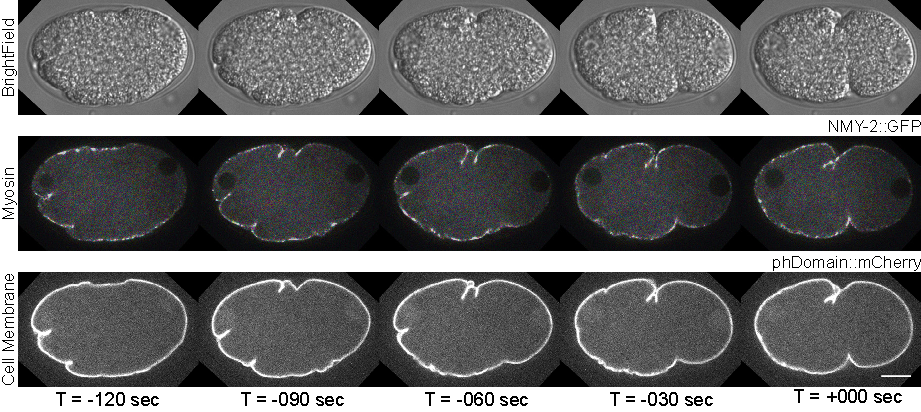
\includegraphics[width=\textwidth]{ExpMethods/FigChannelImages/swg70.pdf}
    \caption{Microscope images of an embryo of SWG070 strain acquired during time-lapse microscopy, depicting the three channels recorded. Top: Bright field, Middle: \ac{nmy2}::\ac{gfp} (myosin), Bottom: phDomain::mCherry (boundary). The male pronucleus can be visualized as the dark circle in the myosin channel towards the posterior end (right). T = \SI{0}{\second} is set at the end of posteriorisation. Scale bar: \SI{10}{\unitLength}} 
    \label{subfig:imageAcquisition-swg070}
\end{subfigure}
\hfill
\begin{subfigure}{\textwidth}
    \centering
    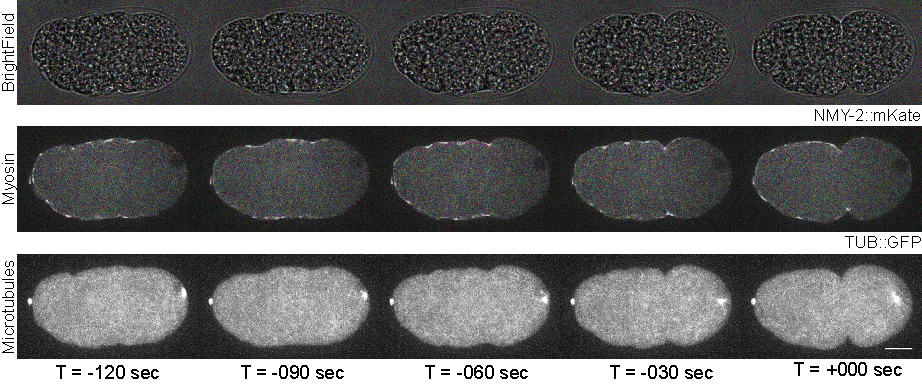
\includegraphics[width=\textwidth]{ExpMethods/FigChannelImages/swg57.pdf}
    \caption{Microscope images of an embryo of SWG057 strain acquired during time-lapse microscopy, depicting the three channels recorded. Top: Bright field, Middle: \ac{nmy2}::mKate (myosin), Bottom: tub::\ac{gfp} (microtubules - we will extract the boundary from this). The male pronucleus can be visualized as the dark circle in the myosin channel towards the posterior end (right). For microtubule channel, the max projection of the z-stack is shown (see \autoref{fig:preprocessSWG057} for example of full z-stack). T = \SI{0}{\second} is set at the end of posteriorisation. Scale bar: \SI{10}{\unitLength}} 
    \label{subfig:imageAcquisition-swg057}
\end{subfigure}
\caption[Image acquisition]{Image acquisition during time-lapse microscopy for SWG070 and SWG057 strain. Images are rotated such that anterior and posterior ends are to the left and right respectively.}
\label{fig:imageAcquisition}
\end{figure}

\section{Image analysis}\label{sec:imageAnalysis}
In this section, we describe the general image analysis pipeline that was used to analyse the movies that were acquired from the microscope. We will mainly focus on movies generated using the SWG070 strain, which will be the primary strain used in this work. However, the analysis pipeline itself can be used for movies from other strains, after certain modifications if needed. For SWG297, since the fluorescent tags are the same, the analysis pipeline can be used without modifications. For SWG057, the pre-processing stage is modified -- which we describe below. Any specific details regarding the analysis of movies generated for a given experiment will be described in the respective sections in \autoref{ch:Results}.

The image analysis pipeline presented here is modified from image analysis pipelines from M. Kramer \citep{mirna2015linking} and P. Gross \citep{gross2019guiding}. The following softwares were used in the image analysis pipeline: \ac{fiji} \citep{schindelin2012fiji,linkert2010metadata} for pre-processing, Python \citep{python38} for tracking the male pronucleus and setting up the inputs for measurements of cortical flows, and \ac{matlab} \citep{MATLAB:2016a} for measurement of cortical and cytoplasmic flows using \acs{piv} and constructing averages of various quantities over the ensemble of embryos in each condition. A custom PowerShell script was used for automated batch processing of movies.

\subsection{Pre-processing}\label{subsec:preprocess}
Movies are pre-processed using a custom \ac{fiji} macro. For each movie, the following steps are performed in order:
\begin{enumerate}
    \item Each movie is cropped to ensure that only a single embryo is present in each frame. If other embryos are present in the cropped frame, they are cleared to black using the \emph{Clear...} command in \ac{fiji}.
    \item Anterior and posterior end of the embryo of interest are manually selected. Posterior side is identified by the depletion of \ac{nmy2} on the posterior end of the cortex. The movie is rotated using bi-linear interpolation such that the anterior and posterior ends of the embryo of interest are on the left and right sides of the frame respectively (see \autoref{subfig:preprocess-manual}).
    \item The pronuclei can be seen as grey circles in the \ac{bf} and dark circles in the \ac{nmy2} channels, located in the cytoplasm. The male pronucleus is identified as the pronucleus towards the posterior end. The movie is flipped to ensure that the male pronucleus is located near the top side of the frame at the start of posteriorization. Any movies with both pronuclei on the same side are discarded  (see \autoref{subfig:preprocess-manual}).
    \item The first frame in the movie at which the male pronucleus appears and the last frame before the male pronucleus moves away from the cortex were manually selected. Only frames between these two selected frames will be analysed  (see \autoref{subfig:preprocess-selectNucleusRange}).
\end{enumerate}

\begin{figure}[h]
\centering
\begin{subfigure}{\textwidth}
    \centering
    \includegraphics[width=0.9\textwidth]{ExpMethods/FigPreProcess/manualAnnotationRotation.png}   \caption{Left image (myosin channel) demonstrates the manual annotation done during pre-processing. Posterior end is recognized by the the presence of the male pronucleus (yellow dotted circle) and the associated depletion of myosin on the cortex. Two points are then marked to denote the posterior and anterior ends respectively (yellow dots near the ends of the embryo). Right image shows the result -- the image is rotated and then flipped (if necessary) to ensure that the anterior and posterior ends are on the left and right of the frame, and that the male pronucleus moves from the top of the embryo towards the posterior end. Scale bar: \SI{10}{\unitLength}} 
    \label{subfig:preprocess-manual}
\end{subfigure}
\hfill
\begin{subfigure}{\textwidth}
    \centering
    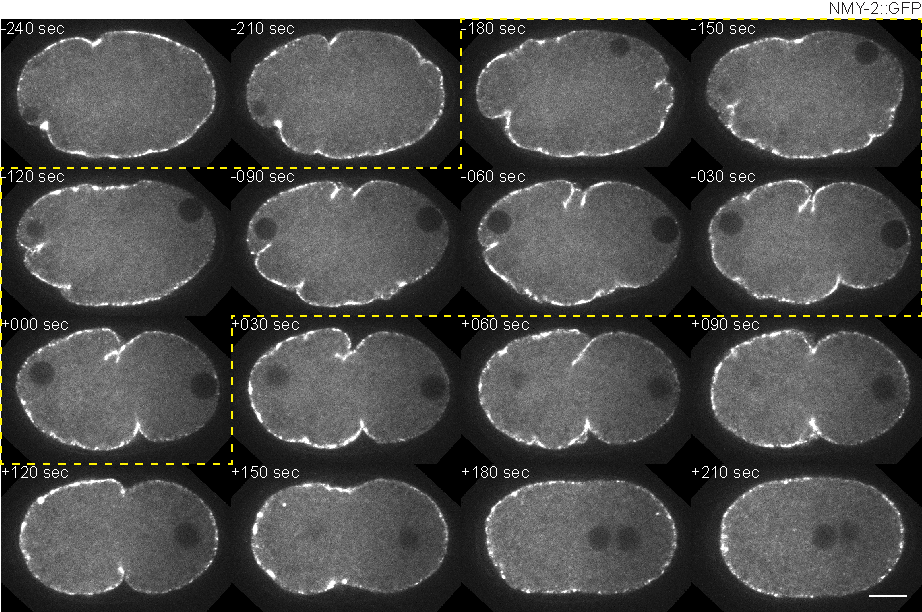
\includegraphics[width=\textwidth]{ExpMethods/FigPreProcess/selectNucleusRange.pdf}
    \caption{Myosin frames at different time-points depicting the movement of the male pronucleus (after rotation and flip). The frame where the male pronucleus first appears is denoted as the first frame. The frame where the male pronucleus starts moving away from the cortex -- and therefore the frame where posteriorisation ends -- is denoted as the last frame. Only the time-points that lie between the first and last frame are analysed (indicated by yellow dotted line). Time-points are denoted in \unit{\second}, with T = \SI{0}{\second} selected as the last frame, i.e. end of posteriorisation. Scale bar: \SI{10}{\unitLength}} 
    \label{subfig:preprocess-selectNucleusRange}
\end{subfigure}
\caption[Image analysis: pre-processing]{Pre-processing steps in the image analysis pipeline, for SWG070 strain. Anterior and posterior are to left and right respectively in all images.}
\label{fig:preprocess}
\end{figure}

For movies generated using SWG057 strain, step 1 of the pre-processing is modified --  see \autoref{fig:preprocessSWG057}. z-stack collected in the \ac{gfp} channel is used to detect the boundary of the embryo of interest in the frame. Kuwahara filter with window size \num{11} is used for noise reduction while still preserving edges \citep{kuwahara1976processing}. The z-stack is thresholded using the default thresholding method used by \ac{fiji} \citep{imageJGuide}. Maximum projection of this binary stack is then used to generate embryo boundary. If multiple embryos are present, only the binary mask corresponding to the embryo of interest is retained. The \ac{bf} images, \ac{nmy2} images and embryo outlines are arranged together in the same channel arrangement as those used for SWG070 movies. After this modification, movies from SWG057 strain are processed in the same as movies from the SWG070 strain.

\begin{figure}[h]
\centering
\includegraphics[width=\textwidth]{ExpMethods/FigPreProcess/swg057BoundaryDetect.png}
\caption[Image analysis: pre-processing (SWG057)]{Modified pre-processing steps for SWG057 strain, to extract embryo boundary from microtubule z-stacks. At each time-point, the z-stack of \num{11} slices in the microtubule channel are filtered using the kuwahara filter, binarized and then max projected. The outline of the max projection is encoded as the boundary channel, mimicking the phDomain::mCherry channel of the SWG070 strain. This outline is shown here as the yellow boundary inscribed onto the myosin frame at the same time-point. Scale bars in all images: \SI{10}{\unitLength}. Anterior and posterior are to left and right respectively in all images.}
\label{fig:preprocessSWG057}
\end{figure}

\subsection{Tracking posteriorisation of the male pronucleus}\label{subsec:nucleusTracking}
To track the position of the male pronucleus as it posteriorises, processed movies were analysed using a custom Python script. Following external packages were used in this Python script: openCV \citep{opencv}, tifffile \citep{tifffile}, scipy \citep{scipy} and numpy \citep{numpy}. This script expects the input movies to be a multipage tiff file with three channels -- first for \ac{bf} (which is not used in analysis), second for \ac{nmy2} and third denoting embryo boundary (example -- phDomain::mCherry in SWG070). We will refer to them as the \ac{bf} channel, the myosin channel, and the boundary channel respectively.

\subsubsection{Segmenting the embryo boundary}\label{subsubsec:boundaryDetect}
For each time-point, the boundary channel frames are extracted and smoothed using a gaussian filter (with sigma = \SI{2}{\pixels}). Each frame are then thresholded using the 90th percentile of the intensity values in that frame as the threshold. A morphological closing operation (with disk element of size \SI{17}{\pixels}) is performed on the binary image thus constructed, to close any gaps in the boundary. To detect if the segmented embryo boundary is indeed closed, the inside of the boundary is filled using a binary fill holes operation. If the boundary is not filled, this operation will fill the whole frame instead. Thus, to detect if the boundary was closed, we check if more than \num{80}\% of the frame is filled. If less than \num{80}\% of the frame was filled, the boundary is closed -- which we segment as the contour of non-zero length enclosing the largest area in the frame. If more than \num{80}\% of the frame was filled, we dilate (with disk element of size \SI{18}{\pixels}) the binary frame with the segmented boundary to attempt closing gaps again. If after the dilation, binary fill holes still leads to more than \num{80}\% of the frame being filled, we consider the boundary detection to be failed for this time-point and use the boundary segmented in the previous time-point. Otherwise, the contour of non-zero length enclosing the largest area in the frame after dilation is again considered as the boundary. Boundary segmented at the previous time-point is also used if the boundary segmented at the current frame has a length too different from the previous one.

For each time-point, the segmented boundary is fit to an ellipse and the long and short axes of the fitted ellipse are calculated. To obtain the average axes for the movie, the axes detected for each time-point are averaged. The average direction is found by averaging the unit vectors that denote the instantaneous directions of the axes in each time-point, and the average lengths by averaging the lengths of the instantaneous axes. See \autoref{fig:segmentingEmbryoBoundary} for an example.

Additionally, the myosin channel frames are also denoised using non-local means denoising \citep{buades2011non}, with the following parameters: Filter strength = \SI{3}{\pixels}, template window size = \SI{4}{\pixels}, search window size = \SI{12}{\pixels}. 

\begin{figure}[h]
\centering
\includegraphics[width=\textwidth]{ExpMethods/FigTrackingPipeline/boundaryDetect.png}
\caption[Image analysis: Segmenting embryo boundary]{Boundary detection using the phDomain::mCherry channel in SWG070. At each time-point, the frame (left) is thresholded (middle, see \nameref{subsubsec:boundaryDetect} for details). The thresholded image provides the segmented boundary. An ellipse is fit to this segmented boundary to obtain the instantenous long and short axes (right, yellow line indicates the fitted ellipse). The same process is carried out on movies generated using embryos from the SWG057 strain. Scale bar: \SI{10}{\unitLength}}
\label{fig:segmentingEmbryoBoundary}
\end{figure}

\subsubsection{Segmenting the male pronucleus}\label{subsubsec:nucleusDetect}
The denoised myosin channel frames are utilized for segmenting the male pronucleus. We only consider myosin frames for the time-points in the range selected in \autoref{subsec:preprocess}. In these frames, the pronuclei can be identified as dark circles devoid of myosin in the cytoplasm. The male pronucleus is identified as the one present in the posterior half (steps in \autoref{subsec:preprocess} ensure we always have this). We utilize this difference in intensities between the cytoplasmic myosin and male pronucleus to segment the latter, using successive thresholding. The following steps are undertaken for each myosin frame (that is, at each time-point) to segment the male pronucleus (see \autoref{fig:malePronucleusTrackingPipeline} for an example):
\begin{enumerate}
    \item The segmented embryo boundary is used to create a mask of the interior of the embryo -- in this way, the boundary segmentation is crucial for male pronucleus segmentation, as it allows separating the interior of the embryo from the whole frame.
    \item The set of thresholds to use for successive thresholding is selected, ranging from the \num{5}th to the \num{95}th percentile of the non-zero intensity values in the embryo interior.
    \item For each threshold in the selected range:
    \begin{enumerate}
        \item The frame is thresholded using the selected threshold. Pixels with intensity values below the selected threshold are set to be white (= \num{1}), and rest to black (= \num{0}).
        \item All pixels to the left (or in the anterior half) of the embryo center (determined as the center of the ellipse fit to the boundary) are set to black (= \num{0}). This ensures that we detect only the male pronucleus, which is present to the right (or in the posterior half). A morphological opening operation with disk element of size \SI{5}{\pixels} is performed to remove small regions of white pixels.
        \item The total number of white pixels for this threshold is recorded.
    \end{enumerate}
    \item To detect the thresholds to use for male pronucleus segmentation, the \enquote{knee} of the Number of white pixels vs Thresholds graph is detected. This \enquote{knee} indicates the threshold above which which the number of white pixels for each threshold increase rapidly, indicating that the white pixels are \enquote{flooding} outside the dark circle that denotes the male pronucleus. To detect this \enquote{knee}, at each threshold we calculate a cost function: the square root of the average of differences from the mean of the number of white pixels up until that threshold is calculated. The threshold for which this cost is the lowest is selected as the maximum threshold to be used for male pronucleus segmentation. See \autoref{subfig:malePronucleusTrackingPipeline-successiveThreshold} for an example.
    \item All thresholds upto this maximum threshold calculated in the last step are considered. The male pronucleus is identified as a dark circle. To quantify how circular a segmentation is, we use the circularity measure\footnote{This measure is based on the isoperimeteric inequality: a geometric inequality that relates the surface area (perimeter for 2D) to the volume (area for 2D) of a region. In 2D, it states that the perimeter of any closed curve $L$ is related to the enclosed area $A$ as $L^2 >= 4\pi A$. Thus, in 2D, for all closed curves with the same perimeter, the one enclosing the most area is the circle.} $ = 4\pi\frac{\textrm{Area}}{\textrm{Perimeter}^2}$, where Area and Perimeter are of the segmented section. Circularity is a dimensionless measure that ranges from \num{0} to \num{1}, with \num{1} being a perfect circle. From all segmentations generated by the thresholds considered in this step, we identify the one that has the largest area and circularity as the male pronucleus. See \autoref{subfig:malePronucleusTrackingPipeline-thresholdSelection} for an example.
\end{enumerate}

\begin{figure}[h]
\centering
\begin{subfigure}{\textwidth}
    \centering
    \includegraphics[width=0.9\textwidth]{ExpMethods/FigTrackingPipeline/successiveThreshold.png}
    \caption{Successive thresholding on myosin frame to segment male pronucleus. Top left image is the denoised myosin frame. All pixels outside this contour are ignored for the purposes of thresholding. Rest of the images show the result after thresholding at a specific threshold -- White pixels have intensities below the selected threshold. Yellow contour indicates the segmented boundary for all images. Note that any white pixels in the left half (that is, anterior half) of the embryo are automatically discarded. Threshold = \num{70} is selected for this myosin frame -- see \autoref{subfig:malePronucleusTrackingPipeline-thresholdSelection}. Scale bar: \SI{10}{\unitLength}} 
    \label{subfig:malePronucleusTrackingPipeline-successiveThreshold}
\end{subfigure}
\hfill
\vspace{1mm}
\begin{subfigure}{\textwidth}
    \centering
    \includegraphics[width=\textwidth]{ExpMethods/FigTrackingPipeline/thresholdSelection.png}
    \caption{Automatic threshold selectiong using successive thresholding (see \nameref{subsubsec:nucleusDetect}). Left: Selecting Max Threshold. Blue curve (left y-axis) depicts the number of white pixels in the sense of \autoref{subfig:malePronucleusTrackingPipeline-successiveThreshold} for each threshold. We want to select Max Threshold near the \enquote{knee} of this curve. Red dotted curve (right y-axis) depicts the cost function. Max Threshold is selected as the threshold with the minimum cost. Right: Selecting Threshold. All thresholds upto Max Threshold are considered. For each threshold, the area of the largest contour (that is, boundary of the largest connected component) is calculated (blue curve, left y-axis). Additionally, the circularity of this contour is calculated (red curve, right y-axis). Final selected threshold for this frame is where the area and circularity are both maximised. For this frame, the selected threshold is \num{70}. See \nameref{subsubsec:nucleusDetect} for definitions} 
    \label{subfig:malePronucleusTrackingPipeline-thresholdSelection}
\end{subfigure}
\caption[Image analysis: Segmenting the male pronucleus]{Segmenting the male pronucleus by successive thresholding and automatic selection. Only a single time-point is considered throughout the figure. Anterior and posterior are to left and right respectively in all images.}
\label{fig:malePronucleusTrackingPipeline}
\end{figure}

\subsubsection{Tracking the male pronucleus}\label{subsubsec:nucleusTrack}
Male pronucleus segmentations generated by the process outlined above are filtered to ensure the following:
\begin{itemize}
    \item The centers of consecutive male pronucleus segmentations (consecutive as in two consecutive time-points) do not have a distance exceeding \SI{13}{\pixels}. This ensures that spurious detections which are far from the male pronucleus are ignored. Given that the cortex and cytoplasm flow at speeds around \SIrange{0}{10}{\micro\meter\per\minute} (see \autoref{subsec:corticalFlows}) and the limitation here corresponds to a speed of \SI{27.3}{\micro\meter\per\minute} or more, no true segmentations are ignored.
    \item Segmentations which are too irregular -- that is, with circularity less than \num{0.7} --  are ignored.
    \item Segmentations which are very small -- that is, with area less than \SI{200}{\pixels^2} --  are ignored.
\end{itemize}
For frames where the segmentations are ignored, an estimate is generated by linearly interpolating between the two closest \enquote{good} frames, where the segmentations were not ignored. This is only done for gaps of \num{5} frames or less, and is not done at the edges of the set of frames selected for nucleus segmentation. The set of male pronucleus segmentations thus generated, as a function of time-points of each frame, constitute the detected trajectory of the male pronucleus in this movie.  

Both the male pronucleus trajectory and the embryo boundary detected using the above analyses are manually verified -- see \autoref{fig:validateSegmentations}. If a movie fails to detect any embryo boundary, or fails to detect the male pronucleus in more than \num{30}\% of frames selected, the movie is discarded.

Following attributes of the trajectory are calculated for each frame (see \autoref{fig:malePronucleusTrackingResults} and \autoref{fig:malePronucleusTrackingVelocities}):
\begin{description}
    \item[Pronucleus position]\hfill\\
    Calculated with respect to the embryo center, designated as origin. The x and y coordinates of the center of the pronucleus, and the polar angle between the long axis and the line connecting the center of the embryo to the center of the pronucleus are stored. We refer to this angle as the \enquote{Angular Position of the male pronucleus}.
    \item[Pronucleus Size]\hfill\\
    Calculated as the total number of pixels in the male pronucleus segmentation at each time-point.
    \item[Distance from cortex]\hfill\\
    Calculated as the distance between the center of the male pronucleus and the closest point on the embryo boundary (cortex).
    \item[Pronucleus velocity]\hfill\\
    Calculated as the gradient of the position of the male pronucleus. The component of the velocity along the x and y axes are stored. Additionally, components of the velocity parallel and perpendicular to the embryo boundary are also calculated. We refer to the component of the pronucleus velocity parallel to the embryo boundary as the \enquote{Posteriorisation velocity}.
\end{description}

\begin{figure}[h]
\centering
\includegraphics[width=\textwidth]{ExpMethods/FigTrackNucleus/validate.pdf}
\caption[Image analysis: Validation]{Validating the results of the segmentations, for different time-points. In each image, the outer yellow contour denotes the fitted ellipse to the segmented boundary, and the inner yellow contour denotes the segmented male pronucleus. Scale bar: \SI{10}{\unitLength}. Anterior is to the left and posterior to the right in all images. T = \SI{0}{\second} denotes end of posteriorisation.}
\label{fig:validateSegmentations}
\end{figure}

\begin{figure}[h]
\centering

\begin{subfigure}[t]{0.45\textwidth}
    \centering
    \includegraphics[width=\textwidth]{ExpMethods/FigTrackNucleus/trajectory.pdf}
    \caption{Trajectory of the male pronucleus -- denoted by the coordinates of its center -- as it posteriorises over time. Color represents time. x- and y-axes lie along the long and short axes of the ellipse fitted to the embryo boundary. Angular position is defined as the angle between the long axis and line connecting the centers of the male pronucleus and embryo.} 
    \label{subfig:malePronucleusTrackingResults-trackPronucleus}
\end{subfigure}
\hfill
\begin{subfigure}[t]{0.45\textwidth}
    \centering
    \includegraphics[width=\textwidth]{ExpMethods/FigTrackNucleus/angularPosVsTime.pdf}
    \caption{Plot of Angular position of the male pronucleus (y-axis) as a function of time (x-axis).} 
    \label{subfig:malePronucleusTrackingResults-angularPosVsTime}
\end{subfigure}

\begin{subfigure}[t]{0.45\textwidth}
    \centering
    \includegraphics[width=\textwidth]{ExpMethods/FigTrackNucleus/sizeVsTime.pdf}
    \caption{Plot of the size of the male pronucleus (y-axis) as a function of time (x-axis). Size is measured as the area enclosed by the contour denoting the male pronucleus segmentation.} 
    \label{subfig:malePronucleusTrackingResults-sizeVsTime}
\end{subfigure}
\hfill
\begin{subfigure}[t]{0.45\textwidth}
    \centering
    \includegraphics[width=\textwidth]{ExpMethods/FigTrackNucleus/crtxDistVsTime.pdf}
    \caption{Plot of Distance between the center of male pronucleus and closest point on cortex (y-axis) as a function of time (x-axis).} 
    \label{subfig:malePronucleusTrackingResults-crtxDistVsTime}
\end{subfigure}

\caption[Image analysis: Trajectory of male pronucleus]{Trajectory of the male pronucleus obtained using the image analysis pipeline. For all plots, T = \SI{0}{\second} denotes the end of posteriorisation. All plots are obtained from a single movie of an embryo of SWG070 strain -- same embryo depicted in \autoref{fig:imageAcquisition}, \autoref{fig:preprocess}, \autoref{fig:segmentingEmbryoBoundary}, \autoref{fig:malePronucleusTrackingPipeline} and \autoref{fig:validateSegmentations}}
\label{fig:malePronucleusTrackingResults}
\end{figure}

\begin{figure}[h]
\centering

\begin{subfigure}[t]{0.45\textwidth}
    \centering
    \includegraphics[width=\textwidth]{ExpMethods/FigTrackNucleus/vxVsTime.pdf}
    \caption{Plot of component of the velocity of the male pronucleus along the long axis (y-axis) as a function of time (x-axis). Positive velocity indicates movement towards posterior.} 
    \label{subfig:malePronucleusTrackingVelocities-vxVsTime}
\end{subfigure}
\hfill
\begin{subfigure}[t]{0.45\textwidth}
    \centering
    \includegraphics[width=\textwidth]{ExpMethods/FigTrackNucleus/vyVsTime.pdf}
    \caption{Plot of component of the velocity of the male pronucleus along the short axis (y-axis) as a function of time (x-axis). Positive velocity indicates movement towards the top of the embryo.} 
    \label{subfig:malePronucleusTrackingVelocities-vyVsTime}
\end{subfigure}

\begin{subfigure}[t]{0.45\textwidth}
    \centering
    \includegraphics[width=\textwidth]{ExpMethods/FigTrackNucleus/postVelVsTime.pdf}
    \caption{Plot of the posteriorisation velocity of the male pronucleus (y-axis) as a function of time (x-axis). Posteriorisation velocity is defined as the component of the velocity of the male pronucleus parallel to the cortex. Positive velocity indicates movement towards posterior.} 
    \label{subfig:malePronucleusTrackingVelocities-postVelVsTime}
\end{subfigure}
\hfill
\begin{subfigure}[t]{0.45\textwidth}
    \centering
    \includegraphics[width=\textwidth]{ExpMethods/FigTrackNucleus/perpVelVsTime.pdf}
    \caption{Plot of the component of the velocity of the male pronucleus perpendicular to the cortex (y-axis) as a function of time (x-axis). Positive velocity indicates movement towards the cortex.} 
    \label{subfig:malePronucleusTrackingVelocities-perpVelVsTime}
\end{subfigure}

\begin{subfigure}[t]{0.45\textwidth}
    \centering
    \includegraphics[width=\textwidth]{ExpMethods/FigTrackNucleus/vxVsAngleSmooth.pdf}
    \caption{Plot of component of the velocity of the male pronucleus along the long axis (y-axis) as a function of angular position (x-axis). Values have been smoothed using a sliding average with window of \num{7} frames. Positive velocity indicates movement towards posterior.} 
    \label{subfig:malePronucleusTrackingVelocities-vxVsAngleSmooth}
\end{subfigure}
\hfill
\begin{subfigure}[t]{0.45\textwidth}
    \centering
    \includegraphics[width=\textwidth]{ExpMethods/FigTrackNucleus/postVelVsAngleSmooth.pdf}
    \caption{Plot of posteriorisation velocity of the male pronucleus (y-axis) as a function of angular position (x-axis). Values have been smoothed using a sliding average with window of \num{7} frames. Positive velocity indicates movement towards posterior.} 
    \label{subfig:malePronucleusTrackingVelocities-postVelVsAngleSmooth}
\end{subfigure}

\caption[Image analysis: Trajectory of male pronucleus (velocities)]{Velocities obtained using the image analysis pipeline. For plots against time, T = \SI{0}{\second} denotes the end of posteriorisation. All plots are obtained from a single movie of an embryo of SWG070 strain -- same embryo depicted in \autoref{fig:imageAcquisition}, \autoref{fig:preprocess}, \autoref{fig:segmentingEmbryoBoundary}, \autoref{fig:malePronucleusTrackingPipeline} and \autoref{fig:validateSegmentations}}
\label{fig:malePronucleusTrackingVelocities}
\end{figure}

\subsubsection{Measuring \ac{nmy2} concentrations}\label{subsubsec:myosinConc}
Myosin concentrations in the cytoplasm and cortex can be measured using the boundary segmentations and denoised myosin frames obtained from the Python script. Here we measure them in intensity per pixel units, where intensity is measured in arbitrary units corresponding to the readings from the camera used to record the movies. We consider a region \SI{15}{pixels} wide below the segmented boundary as being at the cortex, while the cytoplasm is considered as the interior region, left after the cortical region is removed. Myosin concentration in each region is estimated as the average intensity per pixel in the corresponding region, averaged over \num{7} consecutive frames (sliding window).

\subsection{Measuring cortical flows}\label{subsec:corticalFlows}
Cortical flows were measured from the denoised myosin frames using a custom \ac{matlab} script, following \cite{gross2019guiding} (\ac{matlab} script written by P. Gross). The script takes as input the boundary segmentations and the denoised myosin frames generated by the Python script, and performs two steps:
\begin{enumerate}
    \item Using the boundary segmentations already made by the Python script, the \ac{matlab} script generates a kymograph of the cortical layer in the myosin frames. The cortical layer is identified as the region starting from the boundary of the embryo and stretching \SI{30}{\pixels} deep inwards.
    \item These kymographs are then used to measure the flow velocity of the cortex as a function of position along the cortex, using \ac{piv} \citep{thielicke2014pivlab}.
\end{enumerate}
See \autoref{fig:crtxFlowMeasurement} for output kymographs and cortical flows, for the example movie considered in this chapter.

\subsubsection{Creating kymographs}\label{subsubsec:kymographs}
For a given myosin frame, its corresponding boundary segmentation (generated by the Python script) is converted into a composite B{\'e}zier curve: a series of B{\'e}zier curves joined end to end. This converts the discrete pixel positions of the boundary segmentation into a smooth curve that represents the embryo boundary. The point on this curve that is on the embryo's long axis and at the posterior end are identified. Starting from this point, additional points are sampled at one pixel size distance between adjacent points on both ends of the curve. Denoting the initial point on the posterior as zero, these points denote the integer distances along the curve, that is integer arclengths. Thus, the composite B{\'e}zier curve is used to define the distance along the cortex -- the arclength axis. 

At each point sampled on the curve, the normal to the curve pointing towards the embryo interior is found. Points are sampled along each normal at one pixel size distance between adjacent points on a normal upto a distance of \SI{30}{\pixels}, and pixel values are interpolated to obtain the estimated intensities at these points. This can be folded out into a thin rectangular \enquote{band}\footnote{The change in length between the outermost points at the boundary and innermost points towards the embryo interior are ignored, as the length of the embryo boundary is much larger than \SI{30}{\pixels}} of points along the embryo boundary. This \enquote{band} is identified as a folded out version of the cortex, calculating for the frame of interest. The long edge of this band is along the arclength axis, while the short edge is perpendicular. 

By taking the maximum intensity value along this perpendicular axis for each point on the arclength axis (maximum projection), and stacking the resultant 1D representations of myosin distributions for each frame in order of time vertically, a visualization known as the kymograph can be generated -- see \autoref{subfig:crtxFlowMeasurement-kymographFullMovie} and \autoref{subfig:crtxFlowMeasurement-kymographPosteriorization}. This kymograph allows visualization of the changes in myosin distributions as a function of time at each position on the cortex.

\subsubsection{\acf{piv}}\label{subsubsec:pivCortex}
\ac{piv} is a method of visualizing flow in fluids and measuring instantaneous flow velocities \citep{raffel1998particle,thielicke2014pivlab}. Under this method, the fluid is seeded with tracer particles which can be illuminated with light. These tracer particles are small enough that they can be assumed to faithfully follow the fluid dynamics. Time-lapse movies of the fluid flow, with the tracer particles illuminated, are taken. Instead of tracking individual particles, the flow field at a given time-point is calculated by cross-correlating sections of the frame at this time-point with the frame at the next section. In detail, the frame at the current time-point is divided into templates of defined sizes. Each template is cross-correlated with the frame at the next time-point by displacing the template upto a maximum distance from its location in the current time-point. Displacement with the largest cross-correlation, divided by the time elapsed between the two frames, is the measured velocity of the fluid at the location of the template. Here we will use a multi-pass \ac{piv} algorithm, which uses templates of different sizes to measure fluid flow at finer resolutions; along with Gaussian fitting of the peak in the cross-correlation to obtain subpixel accuracy. See \cite{raffel1998particle} for a detailed discussion. 

In the case of the cortex, since myosin motors are fluorescently labelled, tracer particles are not required -- fluorescent tags take the role of the tracer particles. To calculate cortical flow velocities along the arclength axis, the cortical \enquote{bands} extracted for each frame are used for the cross-correlations instead. A multi-pass (4 passes) PIV was utilized, with initial template size of \SI{24}{\pixels} and step size of \SI{4}{\pixels}. Max displacement of each template during cross-correlation was limited to \SI{7}{\pixels}. See \autoref{subfig:crtxFlowMeasurement-crtxFlows} for the measured cortical flows in the example movie considered for this chapter.

\begin{figure}[h]
\centering

\begin{subfigure}[t]{0.45\textwidth}
    \centering
    \includegraphics[width=\textwidth]{ExpMethods/FigCrtxFlows/kymographFullMovie.pdf}
    \caption{Kymograph depicting intensities along the cortex (arclength axis along x-axis) as a function of time (along y-axis), for the full movie. Colorbar indicates the maximum intensity value on the cortex at the given position and time.} 
    \label{subfig:crtxFlowMeasurement-kymographFullMovie}
\end{subfigure}
\hfill
\begin{subfigure}[t]{0.45\textwidth}
    \centering
    \includegraphics[width=\textwidth]{ExpMethods/FigCrtxFlows/kymographPosteriorization.pdf}
    \caption{Kymograph depicting intensities along the cortex (arclength axis along x-axis) as a function of time (along y-axis), only for time-points used to analyze posteriorisation. Colorbar indicates the maximum intensity value on the cortex at the given position and time.} 
    \label{subfig:crtxFlowMeasurement-kymographPosteriorization}
\end{subfigure}

\begin{subfigure}{\textwidth}
    \centering
    \includegraphics[width=0.8\textwidth]{ExpMethods/FigCrtxFlows/crtxFlows.pdf}
    \caption{Cortical flow velocity (colorbar) measured for the time-points used to analyse posteriorization, as a function of time (y-axis) and position along the cortex (x-axis). Positive/Negative flow velocity, depicted in red/blue, indicate movement towards/away from positive end of the arclength axis (x-axis).} 
    \label{subfig:crtxFlowMeasurement-crtxFlows}
\end{subfigure}

\caption[Image analysis: Measuring cortical flows]{Measuring cortical flows. For all plots, T = \SI{0}{\second} on the y-axis denotes the end of posteriorisation, and s = \SI{0}{\unitLength} on the x-axis denotes the posterior pole. All plots are obtained from a single movie of an embryo of SWG070 strain -- same embryo depicted in \autoref{fig:imageAcquisition}, \autoref{fig:preprocess}, \autoref{fig:segmentingEmbryoBoundary}, \autoref{fig:malePronucleusTrackingPipeline} and \autoref{fig:validateSegmentations}}
\label{fig:crtxFlowMeasurement}
\end{figure}

\section{Data analysis}\label{sec:statAnalysis}

This section describes the methods used to analyse the data -- male pronucleus trajectories and cortical flows measured for each embryo -- to obtain ensemble averages for a given experiment. Primarily, we focus on average posteriorization velocity and average cortical flows as a function of angular position of the male pronucleus, for a given experimental condition. All data analysis is done using custom scripts written in \ac{matlab}.

Short-term fluctuations in each male pronucleus trajectory are smoothed using a sliding average with a window of \SI{7}{\frames} for each movie separately. To calculate average posteriorization velocity as a function of angular position, posteriorization velocity and angular positions calculated for all embryos for a given experimental condition are combined together. Angular positions in this dataset are binned in \SI{3}{\unitAngle} bins. Average posteriorization velocity for each angular position bin is calculated by averaging over all posteriorization velocities corresponding to the angular positions included in the bin. \num{95}\% confidence interval for the mean posteriorization velocities are calculated using a two-sided t-test. See \autoref{subfig:dataAnalysisExample-postVel} for an example.

Cortical flows measured for all embryos for a given experimental condition are first aligned using the arclength axis. Cortical flows are then classified using the angular position of the male pronucleus, and binned together in angular position bins of \SI{3}{\unitAngle} width each. Average cortical flows for each angular position bin are calculated by averaging all cortical flows within an angular position bin. Note that this averaging is done spatially: that is, measured flow velocities at the same position on the arclength axis corresponding to different frames are averaged together. The model described in \autoref{ch:ActiveMatter} uses these averaged cortical flows for calibration. See \autoref{subfig:dataAnalysisExample-crtxFlow} for an example.

\begin{figure}[h]
\centering

\begin{subfigure}[t]{0.45\textwidth}
    \centering
    \includegraphics[width=\textwidth]{ExpMethods/FigDataAnalysis/postVel.pdf}
    \caption{Binning Posteriorization velocity (y-axis) vs Angular position (x-axis). Each angular position bin is of \SI{3}{\unitAngle} width. For each bin, the mean posteriorization velocity (dark circles) and 95\% confidence intervals of the mean (error bars) are depicted. Open circles denote the datapoints obtained after smoothing via sliding average (window: \num{7} frames). Dotted line indicates zero posteriorization velocity.} 
    \label{subfig:dataAnalysisExample-postVel}
\end{subfigure}
\hfill
\begin{subfigure}[t]{0.5\textwidth}
    \centering
    \includegraphics[width=\textwidth]{ExpMethods/FigDataAnalysis/crtxFlow.pdf}
    \caption{Binning Cortical flow velocity (colorbar) using Angular position (y-axis). Each angular position bin is of \SI{3}{\unitAngle} width. For each bin, the mean cortical flow at each position along the cortex (x-axis) is calculated -- using all frames that fall within the angular position bin. Positive/Negative flow velocity, depicted in red/blue, indicate movement towards/away from positive end of the arclength axis (x-axis). s = \SI{0}{\unitLength} on the x-axis denotes the posterior pole.} 
    \label{subfig:dataAnalysisExample-crtxFlow}
\end{subfigure}

\caption[Data Analysis (example movie only)]{Data analysis done for a single movie of an embryo of SWG070 strain -- depicted in \autoref{fig:imageAcquisition}, \autoref{fig:preprocess}, \autoref{fig:segmentingEmbryoBoundary}, \autoref{fig:malePronucleusTrackingPipeline} and \autoref{fig:validateSegmentations}. This figure showcases the two main output graphs we obtain from our data analysis.}
\label{fig:dataAnalysisExample}
\end{figure}

\chapter{Experimental investigation of \acs{ap} axis alignment}\label{ch:Results}
In this chapter, we describe the results from the various experiments conducted to investigate the mechanism of \ac{ap} axis alignment, along with their comparisons to the numerical simulations of the theoretical model of \ac{ap} axis alignment described in \autoref{ch:ActiveMatter}. This chapter follows \citep{} closely, with experiments performed by me, P. Gross and M. Kramer; and numerical simulations by M. Nestler. 

\section{Characterising \acs{ap} axis alignment in unperturbed embryos} \label{sec:apAxisAlignCharacteriseWT}
We first set out to characterise the \ac{ap} axis alignment process in unperturbed embryos. \enquote{Unperturbed} here refers to no genetic perturbations, such as no \ac{rnai} or mutations, apart from the addition of fluorescent tags. To this end, we undertook time-lapse microscopy of embryos from the SWG070 strain, which is labelled with \flurophoreLabel{\ac{nmy2}}{\ac{gfp}} and \flurophoreLabel{phDomain}{mCherry}. In these embryos, the male pronucleus can be observed as a dark circle in the cytoplasm, in the \flurophoreLabel{\ac{nmy2}}{\ac{gfp}} fluorescent channel -- as cytoplasmic myosin is excluded from the proncleus. The posterior domain as the depletion of \ac{nmy2} on the cortex near the male pronucleus. We characterise the \ac{ap} axis alignment process by tracking the position of the male pronucleus as it undergoes posteriorisation. We refer the reader to \autoref{sec:imageAnalysis} for details on the image analysis methods used to track the male pronucleus. 

We quantify two aspects of the posteriorisation of the male pronucleus -- its \enquote{angular position} and \enquote{posteriorisation velocity} (see \autoref{sec:imageAnalysis}). Angular position refers to the angle made between the long axis and the line connecting the center of the male pronucleus to the center of the embryo. Posteriorisation velocity is the component of the velocity of the male pronucleus that is parallel to the cortex (at the given angular position). Negative posteriorisation velocities indicate movement in direction of decreasing angular positions and thus towards the posterior end, positive posteriorisation velocity in direction of increasing angular positions and thus away from the posterior end. We also denote the end of posteriorisation as T = \SI{0}{\second}, and synchronise all movies to this time-point. 

Plotting the angular position as a function of time, we find that the angular positions generally decrease towards \SI{0}{\unitAngle} as time reaches closer to end of posteriorisation (T = \SI{0}{\second}). In embryos where the \ac{ap} axis is mis-aligned -- that is, with initial angular position greater than \SI{5}{\unitAngle} (\num{33} out of \num{57} embryos) -- the \ac{ap} axis re-aligns back towards the long axis. We thus confirm the observation made in \cite{goldstein1996specification} -- the \ac{ap} axis does align itself towards the long axis of the embryo, evidenced by the posteriorisation of the male pronucleus.

Plotting the posteriorisation velocity as a function of angular position (see \autoref{sec:statAnalysis} for details on binning), we find that the male pronucleus is, on average, moving towards the posterior end -- with higher speed at higher angular positions. This can also be observed as increasing magnitude of slope of the angular position vs time plots for higher angular positions. We thus conclude that the rate of \ac{ap} axis alignment is faster at higher angular positions: the male pronucleus moves faster towards the posterior end the further away from the posterior end it is.

We also measure the cortical flows in the unperturbed embryos -- see \autoref{sec:imageAnalysis} for methods. We observe an average cortical speed of \SI{4.12 +- 0.59}{\unitCrtxVel}. We also bin the observed cortical flows using angular positions of the male pronucleus -- see \autoref{sec:statAnalysis}. We find that the point where the cortical flows change sign correlates with the angular position, as expected from the mechanism of \ac{ap} axis establishment. These observed cortical flows are later used by the model of \ac{ap} axis alignment described in \autoref{ch:ActiveMatter} for calibration, to generate theoretical values of posteriorisation velocity as a function of angular positions -- see \autoref{subsec:expVsTheoryPcFurrow}.

\section{Cortical flows are required for \acs{ap} axis alignment}\label{sec:corticalFlowsRoleMlc4}
As discussed in \autoref{sec:ApAxisEstablishment}, cortical flows play an important role in proper \ac{ap} axis establishment. Do cortical flows also play a role in \ac{ap} axis alignment? To answer this question, we sought to impair cortical flows, and observe if posteriorisation of the male pronucleus is affected. We perform a \ac{rnai} of \geneExp{mlc-4} on worms of SWG070 strain, for a feeding time of \SI{24}{\unitRNAiTime}, to reduce cortical flow velocity (see \autoref{sec:rnaiMethods} for details on \ac{rnai}). MLC-4 is a conserved regulatory light chain present in \ac{nmy2}, and is required for the \ac{nmy2} myosin motor to function \citep{shelton1999nonmuscle}. We find that cortical flows are indeed reduced in \geneExp{mlc-4} \ac{rnai} embryos -- we observe an average cortical flow speed of \SI{1.45 +- 0.30}{\unitCrtxVel} in \geneExp{mlc-4} \ac{rnai} embryos compared to \SI{4.12 +- 0.59}{\unitCrtxVel} in unperturbed control embryos.

In \geneExp{mlc-4} \ac{rnai} embryos, the male pronucleus was manually tracked instead of being tracked using the image analysis pipeline described in \autoref{sec:imageAnalysis}. We find that the posteriorisation of the male pronucleus is suppressed in these \ac{rnai} embryos: from \num{18} out of \num{30} \ac{rnai} embryos in which the male pronucleus has an initial angular position greater than \SI{5}{\unitAngle}, \num{10} fail to posteriorize. We also observe almost no change in angular position of the male pronucleus in \ac{rnai} embryos over time, as well as very small posteriorisation velocities over different angular positions compared to those observed in unperturbed embryos. We thus conclude that cortical flows are essential for posteriorisation of the male pronucleus, and thus \ac{ap} axis alignment.

\section{Role of Pseudocleavage furrow in \acs{ap} axis alignment}\label{sec:PcFurrowRole}
In this section, we aim to understand the role of the pseudocleavage furrow in the \ac{ap} axis alignment process. In effect, we evaluate to which degree the two mechanisms described in \autoref{ch:APAxisIntro} and \autoref{ch:ActiveMatter} -- the cytoplasmic flow-dependent mechanism and the pseudocleavage furrow-dependent mechanism -- are important for the \ac{ap} axis alignment process. 

\subsection{Removing Pseudocleavage furrow via \acs{rnai}}\label{subsec:Nop1AndNop1Mel11}
As stated, we want to understand if the pseudocleavage furrow-dependent mechanism plays a significant role in \ac{ap} axis alignment. To do so, we quantify the posteriorisation of the male pronucleus in embryos lacking a pseudocleavage furrow. To generate such embryos, we perform a \ac{rnai} of \geneExp{nop-1} on worms of SWG070 strain, for a feeding time of \SI{24}{\unitRNAiTime} (see \autoref{sec:rnaiMethods} for details on \ac{rnai}). NOP-1 modulates activity of the small GTPase RHO-1, which is a major regulator of the activity of the actomyosin cortex in the \ac{ce} embryo \citep{tse2012nop1}. Embryos generated by worms which are mutant for NOP-1 (that is, possess a non-functional form of NOP-1) lack a pseudocleavage furrow \citep{rose1995pseudocleavage}. We find that the \ac{rnai} does indeed generate pseudocleavage furrow-deficient embryos. We also find that \ac{ap} axis alignment is suppressed in the \geneExp{nop-1} \ac{rnai} embryos: these embryos exhibit slower posteriorization velocity compared to unperturbed embryos at different angular positions, with angular positions slowly decaying towards \SI{0}{\unitAngle}. However, we also observe that average cortical flow speed is reduced in these \ac{rnai} embryos: \SI{4.12 +- 0.59}{\unitCrtxVel} in \ac{rnai} embryos compared to \SI{4.12 +- 0.59}{\unitCrtxVel} in unperturbed embryos.

Similar features are observed in the pseudocleavage-furrow deficient embryos generated using worms which are mutant for NOP-1. Using embryos from the SWG228 strain -- which is mutant for NOP-1 and is labelled with \flurophoreLabel{\ac{nmy2}}{\ac{gfp}} -- we observe slower posteriorisation velocity and suppressed changes in angular positions, along with slower cortical flows (\SI{4.12 +- 0.59}{\unitCrtxVel} in \ac{rnai} embryos compared to \SI{4.12 +- 0.59}{\unitCrtxVel} in unperturbed embryos).

Since we have already shown that cortical flows are required for \ac{ap} axis alignment, we sought to generate pseudocleavage furrow-deficient embryos with cortical flows comparable to those observed in unperturbed embryos (which have a pseudocleavage furrow). To generate such embryos, we perform a double \ac{rnai} of \geneExp{nop-1} and \geneExp{mel-11} on worms of SWG070 strain, for a feeding time of \SI{24}{\unitRNAiTime} (see \autoref{sec:rnaiMethods} for details on double \ac{rnai}). MEL-11 is a myosin phosphatase \citep{piekny2002rho} that suppresses the activity of myosin in the cortex \citep{najafabadi2022orchestrating}. We find that embryos generated using this double \ac{rnai} method lack a pseudocleavage furrow. Additionally, these double \ac{rnai} embryos have an average cortical flow speed of \SI{3.34 +- 0.52}{\unitCrtxVel}, comparable to those observed in unperturbed embryos (\SI{4.12 +- 0.59}{\unitCrtxVel}). We also find that the posteriorisation of the male pronucleus is reduced in these double \ac{rnai} embryos: evidenced by a slow change in angular position and slower posteriorisation velocities compared to unperturbed embryos. Furthermore, the posteriorisation of the male pronucleus in these double \geneExp{nop-1; mel-11} \ac{rnai} embryos is comparable to that observed in the single \geneExp{nop-1} \ac{rnai} embryos -- the change in cortical flow speed only marginally effected the posteriorisation of the male pronucleus. However, the male pronucleus in these pseudocleavage-deficient does posteriorise, albeit slowly compared to unperturbed embryos.

Altogether, these experimental results lead us to conclude that the pseudocleavage furrow plays a role in the proper alignment of the \ac{ap} axis at the rate observed in the unperturbed embryos, but is not essential for \ac{ap} axis alignment. Embryos deficient in the pseudocleavage furrow can still exhibit \ac{ap} axis alignment, albeit at a slower rate.

%Motivation: What role does pseudocleavage furrow play in \ac{ap} axis alignment?
%Question: Is \ac{ap} axis alignment reduced by removing pseudocleavage furrow?
%Experiment 1: Remove PC using \textit{nop-1} \ac{rnai}. Refer to RNAi methods
%Observations 1: Cortical flows are reduced - compare to WT here (and refer to mlc-4). Posteriorization velocities are decreased - compare to WT %(refer to figure). Angular position decay slowly to zero. 
%Add. Observation 1: Reduced nematic order in nop-1 (from reymann et al).
%Requirement: Need to get cortical flows close to WT atleast
%Experiment 2: Remove PC using \textit{nop-1} \ac{rnai}, using \textit{mel-11} RNAi to boost cortical flows. Refer to RNAi methods
%Observations 2: Cortical flows are slightly reduced - compare to WT here (and refer to nop-1). Posteriorization velocities are decreased - compare to WT and nop-1 (refer to figure). Angular position decay less slowly to zero. Histograms
%Conclusion: Removing PC reduces \ac{ap} axis alignment rate.

\subsection{Comparing numerical simulations to experimental results}\label{subsec:expVsTheoryPcFurrow}
\subsubsection{Full model accounts for \acs{ap} axis alignment in unperturbed controls}\label{subsubsec:fullModelForWT}
To further probe the role of the pseudocleavage furrow in \ac{ap} axis alignment, we turn to the theoretical model described in \autoref{ch:ActiveMatter}. As described there, the theoretical model considers two possible models of \ac{ap} axis alignment: cytoplasmic flow-dependent mechanism, and the pseudocleavage furrow-dependent mechanism. We aim here to evaluate the contributions of the two mechanisms to the posteriorisation of the male pronucleus in the unperturbed embryos. As these embryos exhibit a pseudocleavage furrow, we consider both mechanisms -- that is, we use the full model. Note that we use the average axes lengths of the unperturbed embryos as the axes length of the ellipsoid used in the theoretical model: \longAxisLength = \SI{28.7}{\unitLength} (semi-major axis), \shortAxisLength = \SI{16.4}{\unitLength} (semi-minor axes) -- see \autoref{sec:imageAnalysis} for methods.

To calibrate our model (see \autoref{ch:ActiveMatter}), we use the experimentally measured cortical flows in unperturbed embryos (see \autoref{subsec:corticalFlows}) for methodology). Specifically, we vary the model parameters -- hydrodynamic length \hydrodynamicLength, active force relaxation \activeRelaxLength and nematic stress relaxation \nematicLength -- until the cortical flows calculated by numerical simulations match the cortical flows observed in the experiments. This is done for a range of angular positions of the male pronucleus, using the average cortical flows observed for angular position bin (with bin width of \SI{3}{\unitAngle} -- see \autoref{sec:statAnalysis} for details on methodology). As the number of movies that exhibit angular positions beyond \SI{21}{\unitAngle} drops below, we only consider angular positions in the range \SIrange{0}{21}{\unitAngle} for calibration of the theoretical model. We find that, after the calibration, the calculated cortical flows match the experimentally observed cortical flows for the following set of model parameters: \hydrodynamicLength = \SI{10}{\unitLength}, \activeRelaxLength = \SI{11.5}{\square\unitLength\per\second}, \nematicLength = \SI{152.5}{\square\unitLength\per\second}. 

In the theoretical model, bulk cytoplasmic flows are determined uniquely from the calculated cortical flows via the no-slip boundary condition (see \autoref{ch:ActiveMatter}). We compare these calculated cytoplasmic flows -- using the calibrated model parameters -- to those observed in the unperturbed embryos (see \autoref{subsec:cytoFlows} for methodology), and find that the calculated cytoplasmic flows show good agreement with experimental cytoplasmic flows over a range of angular positions of the male pronucleus. From these comparisons, we conclude that the theoretical model can faithfully recapitulate the experimental cortical and cytoplasmic flows, for the selected set of model parameters.

We now compare the experimentally observed posteriorisation of the male pronucleus with that calculated in the numerical simulations using the calibrated model. To calculate the posteriorisation velocity of the male pronucleus, the sole remaining model parameter -- drag coefficient \dragCoefficient reflecting direct interactions between the male pronucleus and the cortex (see \autoref{ch:ActiveMatter}) --  is needed. For the set of model parameters obtained via calibration (described above), we set \dragCoefficient = \num{0.61} to ensure that the calculated posteriorisation velocity best match the observed posteriorization velocity as a function of angular position of the male pronucleus. With these model parameters, we find that the calculated posteriorisation velocity agree with experimentally observed average posteriorisation velocity in unperturbed embryos, for angular position upto \SI{21}{\unitAngle}. For higher angular positions, average posteriorisation velocity observed in experiments is faster compared to calculated posteriorisation velocity for the same angular position. By integrating the calculated posteriorisation velocity (as a function of angular position), we obtain a calculated trajectory of the male pronucleus -- referring to the calculated angular position of the male pronucleus as a function of time to posteriorisation. We set the calculated trajectory to be at \SI{0}{\unitAngle} angular position at the end of posteriorisation. We find that the calculated trajectory agrees well with our experimentally observed trajectories of the male pronucleus. 

Additionally, we investigate the sensitivity of the model parameters selected here, with respect to the change in calculated posteriorisation velocity. Specifically, we separately set \hydrodynamicLength, \nematicLength, \activeRelaxLength and \dragCoefficient to $\pm$\num{50}\% of their fitted values, and calculate the posteriorisation velocity. We refer here to these instances of the model with one varied parameter as varied models. On comparison of the calculated posteriorisation velocity, we observe that the varied models still retain the same qualitative behaviour as that exhibited by the calibrated model. Posteriorisation velocity calculated by the varied models for angular positions upto \SI{21}{\unitAngle} remain comparable to the average posteriorisation velocity observed in experiments. Posteriorisation velocity calculated by the varied models for higher angular positions are slower than the average posteriorisation velocity observed in experiments. We also observe that largest variation in calculated posteriorisation velocity is due to variation in \nematicLength -- with larger values of \nematicLength leading to faster posteriorisation velocity. Note that \nematicLength is the model parameter that controls the contribution of the pseudocleavage-furrow dependent mechanism in the theoretical model, as described in \autoref{ch:ActiveMatter}.

Of note also is the hydrodynamic length \hydrodynamicLength, whose value have been measured in previous studies \citep{saha2016determining,mayer2010anisotropies}. We observe here a hydrodynamic length of \hydrodynamicLength = \SI{10}{\unitLength} for the unperturbed embryo, which is close to the previous measurements of the hydrodynamic length ($\sim$\SI{14}{\unitLength} \citep{saha2016determining,mayer2010anisotropies}). Additionally, our analysis above indicates that the calculated posteriorisation velocity is robust towards variation in \hydrodynamicLength. Thus, the calibrated hydrodynamic length used in our theoretical model is in agreement with the previously observed measurements of the hydrodynamic length of the cortex. 

Altogether, we conclude that the full model (with both mechanisms included), using the set of parameters selected here, can -- both qualitatively and quantitatively -- recapitulate the observed \ac{ap} axis alignment process in the unperturbed embryos, for angular positions upto \SI{21}{\unitAngle}. We will refer to the model evaluated with this set of model parameters as the unperturbed model.

\subsubsection{Eliminating role of pseudocleavage furrow-dependent mechanism in model broadly captures the slower \acs{ap} axis alignment in pseudocleavage furrow-deficient embryos}\label{subsubsec:cytoModelForNop1Mel11}
We next investigate if the model can recapitulate the observed posteriorisation of the male pronucleus in the pseudocleavage furrow-deficient embryos generated using \geneExp{nop-1; mel-11} \ac{rnai}. To mimic the experimental removal of the pseudocleavage furrow in the model, we fix \nematicLength -- the model parameter that controls the contribution of the pseudocleavage-furrow dependent mechanism in the model -- to \SI{0}{\square\unitLength\per\second}. Due to this, and since the cortical flows in these embryos are similar but not identical to those observed in unperturbed embryos, we calibrate the model again to ensure we capture the cortical flow velocity observed in the double \ac{rnai} embryos. Doing so yields the following model parameters: \hydrodynamicLength = \SI{11}{\unitLength}, \activeRelaxLength = \SI{7}{\square\unitLength\per\second}, \nematicLength = \SI{0}{\square\unitLength\per\second}. We retain the same value for the drag coefficient \dragCoefficient = \num{0.61} as determined for the unperturbed embryos. We will refer to the model evaluated with this set of model parameters as the pseudocleavage furrow-deficient model.

We compare the posteriorisation velocity calculated using the unperturbed model and the pseudocleavage-deficient model. We find that at each angular position, the pseudocleavage furrow-deficient model calculates slower posteriorisation velocity compared to the unperturbed model -- with the difference larger for higher angular positions. This is qualitatively similar to what was observed experimentally observed -- pseudocleavage furrow-deficient embryos exhibit slower average posteriorisation velocities compared to unperturbed embryos. Furthermore, we find that the fold change (ratio between the compared quantities) between the posteriorisation velocity calculated using the two models -- unperturbed and pseudocleavage-deficient -- is close to fold change between the experimentally observed average posteriorisation velocity in the unperturbed and pseudocleavage furrow-deficient embryos. However, on direct comparison between the calculated posteriorisation velocity from the pseudocleavage furrow-deficient embryos and experimentally observed average posteriorisation velocity in pseudocleavage furrow-deficient embryos, we find that the model calculates slower posteriorisation velocity for all angular positions considered here. Note that the calculated posteriorisation velocity is still comparable to the experimentally observed average posteriorisation velocity in pseudocleavage furrow-deficient embryos. This is further evidenced by comparing the male pronucleus trajectory calculated using the pseudocleavage furrow-deficient embryo with the experimentally observed male pronucleus trajectories. We calculate the male pronucleus trajectory for the pseudocleavage furrow-deficient model in the same fashion as done for the unperturbed model. We find that the calculated trajectory using the pseudocleavage furrow-deficient model agrees well with experimentally observed trajectories in the pseudocleavage-deficient embryos generated using \geneExp{nop-1; mel-11} \ac{rnai}.

We thus conclude that the posteriorisation of the male pronucleus calculated using the pseudocleavage furrow-deficient model -- where \nematicLength is set to \SI{0}{\square\unitLength\per\second} -- is comparable to the experimentally observed posteriorisation in the \geneExp{nop-1; mel-11} \ac{rnai} embryos. The unperturbed and pseudocleavage furrow-deficient models capture the fold change between the unperturbed and double \ac{rnai} embryos. However, the pseudocleavage furrow-deficient model predicts slightly slower posteriorisation than observed in the \geneExp{nop-1; mel-11} \ac{rnai} embryos.

%Note that pseudocleavage furrow is set to zero in model. Cortical flow calibration for nop-1/mel-11 embryos. Why do again calibration: because cortical flows are similar but not same. Show parameters. Comparison for posteriorization velocity and angular position with theory results - in that order. Conclusion: similar order, seems to capture behaviour.
\subsubsection{Suppressed pseudocleavage furrow-dependent mechanism better explains \acs{ap} axis alignment in pseudocleavage furrow-deficient embryos}\label{subsubsec:reducedPcModelForNop1Mel11}
We have reduced the expression of \geneExp{nop-1} (via \ac{rnai}) in order to generate pseudocleavage furrow-deficient embryos. Given that the pseudocleavage furrow-dependent mechanism arises due to the nematic nature of the cortex (see \autoref{ch:ActiveMatter}), we look into the effect \geneExp{nop-1} \ac{rnai} has on nematic order in the cortex. \ac{rnai} of \geneExp{nop-1} reduces the nematic order of the cortex, as measured in \cite{reymann2016cortical} by characterising the orientation of actin filaments. However, note that the cortex in these embryos still retains a weak nematic nature.

Motivated by this observation, we ask if recalibrating the model for the pseudocleavage furrow-deficient embryos generated using \geneExp{nop-1; mel-11} \ac{rnai} while allowing \nematicLength to be non-zero would help explain the discrepancy between the experimentally observed average posteriorisation velocity in the double \ac{rnai} embryos and calculated posteriorisation velocity from the pseudocleavage furrow-deficient embryos. We thus recalibrate the model using the cortical flows experimentally observed in pseudocleavage furrow-deficient embryos , and allowing \nematicLength to vary during the recalibration. We still retain the drag coefficient \dragCoefficient = \num{0.61} -- same as used for the unperturbed model. Doing so yields the following model parameters: \hydrodynamicLength = \SI{11}{\unitLength}, \activeRelaxLength = \SI{7}{\square\unitLength\per\second}, \nematicLength = \SI{25}{\square\unitLength\per\second}. We will refer to the model evaluated with this set of model parameters as the weak pseudocleavage furrow model. Note that the change in \nematicLength between the pseudocleavage furrow-deficient model and the weak pseudocleavage furrow model is much smaller ($\sim$\num{20}\%) compared to the difference between the pseudocleavage furrow-deficient model and the unperturbed model. 

We then compare the posteriorisation velocity calculated by the weak pseudocleavage furrow model with the experimentally observed average posteriorisation velocity in pseudocleavage furrow-deficient embryos (generated using \geneExp{nop-1; mel-11} \ac{rnai}). We find that the calculated posteriorisation velocity using the weak pseudocleavage furrow model better match the experimentally observed average posteriorisation velocity in the pseudocleavage furrow-deficient embryos than those calculated by the pseudocleavage furrow-deficient model. Note however that the difference between the posteriorisation velocities calculated using the pseudocleavage furrow-deficient model and the weak pseudocleavage furrow model is much smaller than between either and those calculated using the unperturbed model.

\subsubsection{Pseudocleavage furrow-dependent mechanism is the predominant mechanism for \acs{ap} axis alignment in unperturbed embryos}\label{subsubsec:pcFurrowDominatesConclude}
Using the models presented in the above section, we can now evaluate the importance of the pseudocleavage furrow-dependent mechanism to the \ac{ap} axis alignment process in unperturbed embryos. We make the following observations:
\begin{itemize}
    \item Posteriorisation velocity calculated by the unperturbed model is mostly sensitive to variations in \nematicLength, and is robust against variations in \hydrodynamicLength and \activeRelaxLength. We retain the same \dragCoefficient for all models.
    \item The model parameter with the largest variation between the three models -- unperturbed, pseudocleavage furrow-deficient, and weak pseudocleavage furrow -- is the \nematicLength. In particular, \nematicLength for the unperturbed model is much larger compared to those for the weak pseudocleavage furrow and the pseudocleavage furrow-deficient models. Other model parameters do not vary as much as the \nematicLength between models.
\end{itemize}
Together, these observations indicate that the large difference between the \nematicLength in the unperturbed model and the weak pseudocleavage furrow model explain most of the difference between the experimentally observed average posteriorisation velocity in the unperturbed embryos and the pseudocleavage furrow-deficient embryos (generated using \geneExp{nop-1; mel-11} \ac{rnai}). This similarly follows for the pseudocleavage furrow-deficient model. 

Note that \nematicLength is the model parameter that controls the contribution of the pseudocleavage furrow-dependent mechanism in the model (see \autoref{ch:ActiveMatter}). Also note that the posteriorisation velocity is much slower in the pseudocleavage furrow-deficient embryos compared to unperturbed embryos ($\sim$\num{80}\% slower). Combined with the observations above, we are led to conclude that the pseudocleavage furrow-dependent mechanism provides the major contribution to the posteriorisation velocity observed in the unperturbed embryos, and thus is the predominant mechanism responsible for the proper \ac{ap} axis alignment in the unperturbed embryos. Slow \ac{ap} axis alignment in the pseudocleavage-furrow deficient embryos indicates that the other mechanism -- the cytoplasmic flow-dependent mechanism -- plays a minor role in \ac{ap} axis alignment.

%Note that pseudocleavage furrow is allowed to vary. Cortical flow calibration for nop-1/mel-11 embryos. Comparison for posteriorization velocity and angular position with theory results - in that order. Show parameters. Conclusion: better match, furrow parameter still low compared to unperturbed.

\section{Role of embryo geometry in \acs{ap} axis alignment}\label{sec:GeometryRole}
In this section, we aim to understand the role of embryo geometry in the \ac{ap} axis alignment process. Here, we consider changes in the aspect ratio of the embryo, while still retaining an ellipsoidal geometry. Specifically, we ask how the rate of \ac{ap} axis alignment, measured as the posteriorisation velocity of the male pronucleus, differs between ellipsoidal embryos with different aspect ratios. We define aspect ratio of the embryo as the ratio of the lengths of the long axis 2\longAxisLength and the two equal short axes 2\shortAxisLength~ -- aspect ratio = \aspectRatio. 

\subsection{Rounder embryos show slower \acs{ap} axis alignment}\label{subsec:roundEmbryosIma3}
As stated, we want to understand if and how changes in embryo geometry affect the rate of \ac{ap} axis alignment -- measured here as the posteriorisation velocity of the male pronucleus. The specific change in embryo geometry we consider here is the reduction in aspect ratio of the embryo -- leading to embryos with a more spherical or \enquote{rounder} shape (hence referred to as rounder embryos). 

We first approach this question using numerical simulations of the theoretical model. We use the same model parameters as defined for the unperturbed model (as defined in \autoref{subsec:expVsTheoryPcFurrow}) -- thus, the model parameters chosen are: \hydrodynamicLength = \SI{10}{\unitLength}, \activeRelaxLength = \SI{11.5}{\square\unitLength\per\second}, \nematicLength = \SI{152.5}{\square\unitLength\per\second}, and \dragCoefficient = \num{0.61}. However, we now vary the aspect ratio of the ellipsoid used for the numerical simulation, while keeping the volume of the ellipsoid the same as that used for the unperturbed model (see \autoref{ch:ActiveMatter} for details). Specifically, we consider ellipsoids with the following aspect ratios: \aspectRatio = \num{1.10}, \num{1.25}, \num{1.35}, \num{1.48}, \num{1.58}, \num{1.78}. Note that \num{1.78} is the aspect ratio of the ellipsoid used for the unperturbed model -- corresponding to the average aspect ratio of unperturbed embryos (see below). We calculate the predicted posteriorisation velocity as a function of angular position of the male pronucleus, using each of the aspect ratios listed before and the model parameters set before. As for the unperturbed model, we consider only angular positions upto \SI{21}{\unitAngle}. We find that for each angular position, posteriorisation velocity generally grow faster as the aspect ratio rises -- with larger differences between posteriorisation velocities at higher angular positions. Thus, we conclude that the model predicts that the rate of \ac{ap} axis alignment is related to the aspect ratio of the ellipsoid, and therefore embryo geometry -- with rounder embryos exhibiting slower \ac{ap} axis alignment compared to more ellipsoidal ones. Note that such a prediction is consistent with the extreme case of a perfectly round (or spherical) embryo; since such a spherical embryo lacks any unique long axis, we must expect no \ac{ap} axis alignment in a spherical embryo.

We next verify this prediction experimentally. To do so, we generate rounder embryos by performing a \ac{rnai} of \geneExp{ima-3} on worms of SWG070 strain, for a feeding time of \SI{20}{\unitRNAiTime} (see \autoref{sec:rnaiMethods} for details on \ac{rnai}). IMA-3 is a member of the importin $\alpha$ family of nuclear transport factors \citep{geles2001germline,sonnichsen2005full}. It has been observed in previous studies that \geneExp{ima-3} \ac{rnai} generates rounder and smaller embryos \citep{sonnichsen2005full}. We verify this here by measuring the lengths of the semi-major \longAxisLength and semi-minor \shortAxisLength axes and the aspect ratio of \geneExp{ima-3} \ac{rnai} embryos and comparing them to those measured for the unperturbed embryos (see \autoref{subsec:nucleusTracking} for details). We find that the average axes lengths for the unperturbed embryos was \longAxisLength = \SI{28.7 +- 1.6}{\unitLength} and \shortAxisLength = \SI{16.2 +- 1.1}{\unitLength}, corresponding to an aspect ratio of \aspectRatio = \num{1.78 +- 0.20}. This is compared to the average axes lengths and aspect ratio measured for \geneExp{ima-3} \ac{rnai} embryos, for which we find \longAxisLength = \SI{20.9 +- 2.2}{\unitLength}, \shortAxisLength = \SI{13.8 +- 0.8}{\unitLength} and \aspectRatio = \num{1.48 +- 0.20}. We also note that the average volume of these embryos (calculated for each embryo as the volume of the ellipsoid with the same axes lengths as those measured for the embryo) is smaller in \geneExp{ima-3} \ac{rnai} embryos compared to unperturbed embryos -- indicating \geneExp{ima-3} \ac{rnai} embryos have a smaller volume compared to unperturbed embryos. Therefore, we note that \geneExp{ima-3} \ac{rnai} embryos are, on average, smaller and rounder compared to unperturbed embryos.

We also investigate if the model parameters used for the unperturbed model can be utilized for the \ac{rnai} embryos. Specifically, we compare the measured myosin concentrations in the cytosol and cortex of the \ac{rnai} embryos with those measured in the unperturbed embryos (see \autoref{subsec:nucleusTracking} for methods); and also compare the cortical flows measured in the \ac{rnai} embryos to those measured in the unperturbed embryos. We find that the myosin concentrations in the cytosol and cytoplasm are not significantly different between the \ac{rnai} embryos and the unperturbed embryos. We also find that the average cortical flow speed is not significantly different between the \ac{rnai} embryos and the unperturbed embryos: \SI{4.12 +- 0.59}{\unitCrtxVel} in \ac{rnai} embryos compared to \SI{4.12 +- 0.59}{\unitCrtxVel} in unperturbed embryos. These observations indicate that the cortex of the \ac{rnai} embryos does not differ from the cortex of the unperturbed embryos in any meaningful way. Thus, we conclude that the same model parameters used for the unperturbed model can also be used to calculate predicted posteriorisation velocity for the \geneExp{ima-3} \ac{rnai} embryos.

Having confirmed that the same model parameters as those used for comparison to the unperturbed embryos can be used for comparison to the \geneExp{ima-3} \ac{rnai} embryos, we next use the model to predict the posteriorisation velocity of the male pronucleus for the rounder \ac{rnai} embryos. For the model, we use an ellipsoid with aspect ratio \aspectRatio = \num{1.48}, and the same volume as that used for unperturbed embryos -- yielding semi-major axis of length \longAxisLength = \SI{25.8}{\unitLength} and semi-minor axes of length \shortAxisLength = \SI{17.4}{\unitLength}. Therefore, our model prediction ignores the difference in embryo size between the \ac{rnai} embryos and unperturbed embryos. We compare the posteriorisation velocity calculated using in the numerical simulations of this model to the observed average posteriorisation velocity in the \ac{rnai} embryos as a function of angular positions. We find that the predicted posteriorisation velocity agree with experimentally observed average posteriorisation velocity in \ac{rnai} embryos, for angular position upto \SI{24}{\unitAngle}. For higher angular positions, average posteriorisation velocity observed in experiments is faster compared to predicted posteriorisation velocity for the same angular position. By integrating the predicted posteriorisation velocity (as a function of angular position), we obtain a predicted trajectory of the male pronucleus -- referring to the predicted angular position of the male pronucleus as a function of time to posteriorisation. We set the predicted trajectory to be at \SI{0}{\unitAngle} angular position at the end of posteriorisation. We find that the predicted trajectory agrees well with our experimentally observed trajectories of the male pronucleus for the \ac{rnai} embryos.

We next compare the posteriorisation of the male pronucleus in these \ac{rnai} embryos to that observed in the unperturbed embryos. Comparing the average posteriorisation velocity as a function of angular positions, we observe that the rounder \ac{rnai} embryos exhibits slower average posteriorisation velocity compared to those measured in unperturbed embryos for all angular positions -- with larger differences for higher angular positions. We also observe this in the male pronucleus trajectories, with slower change in angular position as a function of time in \ac{rnai} embryos, compared to unperturbed embryos. Thus, we conclude that rounder \geneExp{ima-3} \ac{rnai} embryos exhibit slower rate of \ac{ap} axis alignment compared to unperturbed embryos -- matching the prediction of the theoretical model. Note also that while the posteriorisation velocity is slower in \geneExp{ima-3} \ac{rnai} embryos compared to those observed in unperturbed embryos, but is faster than those observed in the pseudocleavage furrow-deficient embryos generated by the \geneExp{nop-1; mel-11} \ac{rnai}.

Altogether, these observations lead us to conclude that rounder embryos do indeed show slower rate of \ac{ap} axis alignment -- as predicted by our theoretical model and confirmed experimentally. Since the diminished posteriorisation velocity observed in the rounder \geneExp{ima-3} \ac{rnai} embryos match the posteriorisation velocity predicted by the model using the same aspect ratio as the average aspect ratio observed in \geneExp{ima-3} \ac{rnai} embryos, our model captures this relation between embryo geometry and \ac{ap} axis alignment in a quantitative manner. Additionally, note that the prediction for the \geneExp{ima-3} \ac{rnai} embryos only takes into account the change in aspect ratio of the embryos, yet makes a prediction that matches the experimental observations. Thus, we conclude that the primary feature of embryo geometry that influences \ac{ap} axis alignment is the aspect ratio of the embryo.

%Motivation: How does changing embryo geometry change \ac{ap} axis alignment?
%Question: What happens for rounder embryos - less prominent long axis.
%Prediction: Less prominent long axis implies less prominent alignment. Numerical simulations on rounder embryos with same volumes indicate this is true.
%Experiment: Rounder embryos using ima-3 RNAi. Refer to methods.
%Observations 1: ima-3 embryos are rounder (long axis, short axis, aspect ratio). Same myosin concentrations and cortical flows as WT. Volumes are reduced - 70\%.
%Observations 2: Posteriorization velocities are decreased - compare to WT and nop-1/mel-11 (refer to figure). Angular position does decay slightly slower to zero. Histograms
%Conclusion: Rounder embryos show slower \ac{ap} axis alignment

\subsection{Relation between embryo geometry and \acs{ap} axis alignment}\label{subsec:postVelVsAspectRatio}

\subsubsection{Exploring the relation between aspect ratio and posteriorisation velocity}\label{subsubsec:postVelVsAspectRatioExpAndModel}
Our theoretical model demonstrates a relation between aspect ratio of the embryo and the rate of \ac{ap} axis alignment (measured as posteriorisation velocity of the male pronucleus): slower rate of \ac{ap} axis alignment (that is, slower posteriorisation velocity at different angular positions) for smaller aspect ratios (that is, rounder embryos). We next sought to experimentally evaluate this relation directly. Here, instead of considering the posteriorisation velocity of the male pronucleus as a function of angular position for a given average aspect ratio (as we have done until now), we now consider the posteriorization velocity as a function of aspect ratio, averaged over a range of angular positions. Experimental variation in the aspect ratios of both unperturbed (\numrange{1.6}{2.1}) and \geneExp{ima-3} \ac{rnai} embryos (\numrange{1.1}{1.7}) enables us to evaluate this relation over a broad range of aspect ratios (\numrange{1.1}{2.1}). Since the difference in volume between the unperturbed embryos and \ac{rnai} embryos does not appear to be important for \ac{ap} axis alignment, and that cortical flows and myosin concentrations are not significantly different between unperturbed embryos and \geneExp{ima-3} \ac{rnai} embryos; we combine the two sets of embryos into a single set which we consider here. Thus, the set of embryos considered in this subsection contains both the unperturbed embryos and \ac{rnai} embryos, with no distinction made between the two. We will refer to this set of embryos as the combined set of embryos.

We next proceed to obtain the experimentally observed relation between the posteriorisation velocity of the male pronucleus and aspect ratio of the embryo from the combined set of embryos. To do so, we bin the combined set using aspect ratio, with bin width of \num{0.2}. For each bin, we average over the observed posteriorisation velocity for all angular positions between \SIrange{3}{15}{\unitAngle}. This gives us the average posteriorisation velocity (along with \num{95}\% confidence intervals calculated using two sided t-test) observed for each aspect ratio bin -- thus yielding the experimentally observed relation between the two.

From the numerical simulations done using ellipsoids with different aspect ratios, we can also obtain a relation between the posteriorisation velocity and aspect ratio as predicted by the theoretical model. For each aspect ratio used before, we average the posteriorisation velocity for all angular positions between \SIrange{3}{15}{\unitAngle}. For aspect ratios in-between, we use linear interpolation. This yields us the relation between the posteriorisation velocity and aspect ratio, as calculated using the theoretical model. Comparing to the experimentally observed relation, we find that the theoretical relation matches the experimental one well over a range of aspect ratios from \numrange{1.1}{1.7}.

\subsubsection{Effective model of a contractile ring on an ellipsoid captures the relation between embryo geometry and \acs{ap} axis alignment}\label{subsubsec:effectiveModel}

How does this relation between the embryo geometry (characterised by aspect ratio) and \ac{ap} axis alignment (characterised by posteriorisation velocity) arise? As shown in \autoref{subsec:expVsTheoryPcFurrow}, the predominant mechanism for \ac{ap} axis alignment is the pseudocleavage furrow-dependent mechanism. The pseudocleavage furrow may effectively be considered as a contractile ring, rotating about the equator of an ellipsoid (representing the embryo) during \ac{ap} axis alignment. We here ask if this effective model of a contractile ring on an ellipsoid enough to capture the relation between aspect ratio of the embryo and posteriorisation velocity of the male pronucleus, as observed in the combined set of embryos.

In this effective model, we consider an fixed axi-symmetric ellipsoid of axis lengths [\longAxisLength,\shortAxisLength,\shortAxisLength], with \longAxisLength being the length of the semi-major axis and \shortAxisLength being the length of the two equal semi-minor axes. The semi-major (or long) axis defines the x-axis, while the two semi-major (or short) axes define the y- and z- axes, respectively. On this ellipsoid, we consider a contractile ring which represents the pseudocleavage furrow. The center of the ring and the center of the ellipsoid are coincident (at the origin of the coordinate system). This ring rotates about the z-axis, representing the rotation of the pseudocleavage furrow during \ac{ap} axis alignment. Thus, the contractile ring has only a sole degree of freedom: the angle $\alpha$ made between the normal to the plane of the contractile ring and the x-axis. Since we are only interested in angular positions from \SIrange{3}{15}{\unitAngle}, we only consider small angle $\alpha$ here.

We make the following assumptions in our effective model, with regards to the dynamics of the contractile ring:
\begin{itemize}
    \item The ring has a constant line tension $T$ - independent of both the orientation of the ring ($\alpha$) and the shape of the ellipsoid (\longAxisLength, \shortAxisLength). Here, $T$ has units of force.
    \item The frictional torque acting on the ring is controlled by a frictional coefficient $\gamma$, and is given by $\gamma\cdot\dot{\alpha}$
    \item We do not consider any inertial terms: Torque generated by the ring is perfectly balanced by the torque generated by friction.
\end{itemize}                                                                             
Under the above assumptions, we want to calculate $\dot{\alpha}$ as a function of \longAxisLength, \shortAxisLength and $\alpha$ -- for small angles $\alpha$. Note that \longAxisLength and \shortAxisLength are free to vary - we do not assume that our ellipsoid is close to a sphere.

\paragraph{Motion of contractile ring}
We first consider the mechanical energy stored in the contractile ring, which can be given by:
\begin{equation} \label{eq:energyDef}
    E = TC(\alpha)
\end{equation}
where $C(\alpha)$ is the total circumference of the ring.

To calculate the circumference of the ring for any given $\alpha$, we first write a description of the ring as an intersection of the ellipsoid with the plane in which the ring resides. This plane makes an angle of $\alpha$ with the yz plane, and passes through the origin. Thus, it can be described by the equation: $y = -x\cot\alpha$. The ellipsoid itself can be described as $\frac{x^2}{a^2} + \frac{y^2 + z^2}{b^2} = 1$. On taking the intersection of the ring plane with the ellipsoid, we get the equation describing the ring:
\begin{align*}
    \textrm{Plane: }&y = -x\cot\alpha \\
    \textrm{Ellipsoid: }&\frac{x^2}{a^2} + \frac{y^2 + z^2}{b^2} = 1 \\
    \textrm{Intersection (Ellipse): }&\frac{x^2}{a^2} + \frac{x^2\cot^2\alpha + z^2}{b^2} = 1\\
    &\implies x^2\left(\frac{a^2\cot^2\alpha + b^2}{a^2b^2}\right) + \frac{z^2}{b^2} = 1; \quad y = -x\cot\alpha
\end{align*}
Let us define $A = \frac{ab}{\sqrt{a^2\cot^2\alpha + b^2}}$. Then, the equation in the intersection part above can be written as: $\frac{x^2}{A^2} + \frac{z^2}{b^2} = 1$ - a form similar to the canonical form for an ellipse. Calling the parametric angle for this ellipse $\phi$, we then can write the position vector describing the ring $\Vec{r}$ as:
\begin{equation*}
    \Vec{r} = \left(A\cos\phi,-A\cot\alpha\cos\phi,b\sin\phi\right); \quad A = \frac{ab}{\sqrt{a^2\cot^2\alpha + b^2}}
\end{equation*}
where $\phi \in [-\pi,\pi)$.

Note that the ring is an ellipse in its plane - since the intersection of an ellipsoid and a plane must be an ellipse. This can also be seen by the form by $\norm{\Vec{r}}^2$:
\begin{equation*}
    \norm{\Vec{r}}^2 = A^2(1 + \cot^2\alpha)\cos^2\phi + b^2\sin^2\phi
\end{equation*}

We can therefore calculate semi-major $a_{ring}$ and semi-minor $b_{ring}$ axes of the ellipse formed by the ring. We directly read them off the expression of $\norm{\Vec{r}}^2$ :
\begin{align*}
    a_{ring} &= A\sqrt{1 + \cot^2\alpha} = \frac{ab}{\sqrt{a^2\cot^2\alpha + b^2}}\sqrt{1 + \cot^2\alpha^2} = \frac{ab}{\sqrt{a^2\cos^2\alpha + b^2\sin^2\alpha}}\\
    b_{ring} &= b \\
    e_{ring} &= \sqrt{1 - \left(\frac{b_{ring}}{a_{ring}}\right)^2} = \sqrt{1 - \frac{a^2\cos^2\alpha + b^2\sin^2\alpha}{a^2}} = \sqrt{\sin^2\alpha - \frac{b^2}{a^2}\sin^2\alpha} = \sin\alpha\sqrt{1 - \frac{b^2}{a^2}}
\end{align*}
where $e_{ring}$ is the eccentricity of the ellipse formed by the ring. Note that since the ring rotates about the yz plane (i.e. the plane with the two short axes), the short axis of the ring is just $b$.

The circumference of the ring is then given by the circumference of this ellipse. The formula for the circumference of an ellipse is:
\begin{equation} \label{eq:circum}
    C(\alpha) = 4a_{ring}\int_0^{\frac{\pi}{2}} \sqrt{1 - e_{ring}^2\sin^2\phi} \dd{\phi}
\end{equation}

\paragraph{Torque generated by contractile ring}
Using \eqref{eq:energyDef} and \eqref{eq:circum}, we can write down the energy as:
\begin{align*}
    E &= TC(\alpha) = 4Ta_{ring}\int_0^{\frac{\pi}{2}} \sqrt{1 - e_{ring}^2\sin^2\phi} \dd{\phi}\\
    &= 4T\frac{ab}{\sqrt{a^2\cos^2\alpha + b^2\sin^2\alpha}}\int_0^{\frac{\pi}{2}} \sqrt{1 - \left(1 - \frac{b^2}{a^2}\right)\sin^2\alpha\sin^2\phi} \dd{\phi}
\end{align*}

The torque can then be expressed as:
\begin{align*}
    \tau &= -\dv{E}{\alpha} = -4T\dv{\alpha}\left(\frac{ab}{\sqrt{a^2\cos^2\alpha + b^2\sin^2\alpha}}\int_0^{\frac{\pi}{2}} \sqrt{1 - \left(1 - \frac{b^2}{a^2}\right)\sin^2\alpha\sin^2\phi_{ring}} \dd{\phi_{ring}}\right)\\
    &= -4T\left[\frac{ab(a^2 - b^2)\cos\alpha\sin\alpha}{\left(a^2\cos^2\alpha + b^2\sin^2\alpha\right)^{\flatfrac{3}{2}}}\int_0^{\frac{\pi}{2}} \sqrt{1 - \left(1 - \frac{b^2}{a^2}\right)\sin^2\alpha\sin^2\phi_{ring}} \dd{\phi_{ring}}\right.\\
    &\left.\quad + \frac{ab}{\sqrt{a^2\cos^2\alpha + b^2\sin^2\alpha}}\int_0^{\frac{\pi}{2}} \frac{-\left(1 - \frac{b^2}{a^2}\right)\sin\alpha\cos\alpha\sin^2\phi_{ring}}{\sqrt{1 - \left(1 - \frac{b^2}{a^2}\right)\sin^2\alpha\sin^2\phi_{ring}}} \dd{\phi_{ring}}\right]\\
    &= -4T\frac{ab(a^2 - b^2)\sin\alpha\cos\alpha}{\sqrt{a^2\cos^2\alpha + b^2\sin^2\alpha}}\\
    &\times\int_0^{\frac{\pi}{2}}\left[\frac{1 - \left(1 - \frac{b^2}{a^2}\right)\sin^2\alpha\sin^2\phi_{ring}}{a^2\cos^2\alpha + b^2\sin^2\alpha}-\frac{\sin^2\phi_{ring}}{a^2}\right]\frac{1}{\sqrt{1 - \left(1 - \frac{b^2}{a^2}\right)\sin^2\alpha\sin^2\phi_{ring}}}\dd{\phi_{ring}}\\
    &= -4T\frac{ab(a^2 - b^2)\sin\alpha\cos\alpha}{a^2\sqrt{a^2\cos^2\alpha + b^2\sin^2\alpha}}\\
    &\times\int_0^{\frac{\pi}{2}}\left[\frac{a^2 - \left(a^2 - b^2\right)\sin^2\alpha\sin^2\phi_{ring}}{a^2\cos^2\alpha + b^2\sin^2\alpha}-\sin^2\phi_{ring}\right]\frac{1}{\sqrt{1 - \left(1 - \frac{b^2}{a^2}\right)\sin^2\alpha\sin^2\phi_{ring}}}\dd{\phi_{ring}}\\
    &= -4T\frac{ab(a^2 - b^2)\sin\alpha\cos\alpha}{a^2\sqrt{a^2\cos^2\alpha + b^2\sin^2\alpha}}\\
    &\times\int_0^{\frac{\pi}{2}}a^2\left[\frac{1 - \sin^2\phi_{ring}}{a^2\cos^2\alpha + b^2\sin^2\alpha}\right]\frac{1}{\sqrt{1 - \left(1 - \frac{b^2}{a^2}\right)\sin^2\alpha\sin^2\phi_{ring}}}\dd{\phi_{ring}}\\
    \implies \tau &= -4T\frac{ab(a^2 - b^2)\sin\alpha\cos\alpha}{\left(a^2\cos^2\alpha + b^2\sin^2\alpha\right)^{\flatfrac{3}{2}}}\int_0^{\frac{\pi}{2}}\frac{\cos^2\phi_{ring}}{\sqrt{1 - \left(1 - \frac{b^2}{a^2}\right)\sin^2\alpha\sin^2\phi_{ring}}}\dd{\phi_{ring}}
\end{align*}

Using the Taylor expansion around $\alpha = 0$, we can expand $\tau$ to linear order in $\alpha$ as $\tau = \left.\tau\right|_{\alpha=0} + \left.\dv{\tau}{\alpha}\right|_{\alpha=0}\alpha + \mathcal{O}(\alpha^2)$. Note that on $\alpha = 0$, the torque also goes to zero. To obtain the linear order expansion, we calculate the derivative of the torque at $\alpha = 0$.
\begin{align*}
    \left.\dv{\tau}{\alpha}\right|_{\alpha=0} &= -4T\left.\dv{\alpha}\left[\frac{ab(a^2 - b^2)\sin\alpha\cos\alpha}{\left(a^2\cos^2\alpha + b^2\sin^2\alpha\right)^{\flatfrac{3}{2}}}\int_0^{\frac{\pi}{2}}\frac{\cos^2\phi_{ring}}{\sqrt{1 - \left(1 - \frac{b^2}{a^2}\right)\sin^2\alpha\sin^2\phi_{ring}}}\dd{\phi_{ring}}\right]\right|_{\alpha = 0} \\
    &= -4T \left[\dv{\alpha}\left(\frac{ab(a^2 - b^2)\sin\alpha\cos\alpha}{\left(a^2\cos^2\alpha + b^2\sin^2\alpha\right)^{\flatfrac{3}{2}}}\right)_{\alpha=0}\int_0^{\frac{\pi}{2}}\frac{\cos^2\phi_{ring}}{\sqrt{1 - \left(1 - \frac{b^2}{a^2}\right)(0)\sin^2\phi_{ring}}}\dd{\phi_{ring}}\right.\\
    &\quad + \left.\frac{ab(a^2 - b^2)*0*1}{\left(a^2(1) + b^2(0)\right)^{\flatfrac{3}{2}}}\dv{\alpha}\left(\int_0^{\frac{\pi}{2}}\frac{\cos^2\phi_{ring}}{\sqrt{1 - \left(1 - \frac{b^2}{a^2}\right)\sin^2\alpha\sin^2\phi_{ring}}}\dd{\phi_{ring}}\right)_{\alpha=0}\right]\\
    &= -4T \left[\frac{ab(a^2 - b^2)}{\left(a^2*1 + b^2*0\right)^{\flatfrac{3}{2}}}\right] \int_0^{\frac{\pi}{2}}\cos^2\phi_{ring}\dd{\phi_{ring}} = -4T\frac{ab(a^2-b^2)}{a^3}\frac{\pi}{4}\\
    \implies \left.\dv{\tau}{\alpha}\right|_{\alpha=0} &= -\pi T b\left(1 - \frac{b^2}{a^2}\right)
\end{align*}

Thus, by Taylor expansion, the torque to linear order in $\alpha$ is:
\begin{equation} \label{eq:torque}
    \tau \approx \left.\dv{\tau}{\alpha}\right|_{\alpha=0}\alpha =  -\pi T b\left(1 - \frac{b^2}{a^2}\right)\alpha
\end{equation}

\paragraph{Torque balance for the contractile ring}
Per our assumption of negligible inertial terms and the form of friction experienced by the ring, the torque balance of the ring can be written as:
\begin{equation*}
    \tau - \gamma\cdot\dot{\alpha} = 0
\end{equation*}
Putting in the expression for $\tau$ we just obtained, we get
\begin{equation} \label{eq:alphaDot}
    \dot{\alpha} \approx - \frac{\pi T}{\gamma} b\left[1 - \frac{b^2}{a^2}\right]\alpha
\end{equation}

\paragraph{Calculating posteriorization velocity of the male pronucleus $v$}
To get the posteriorization velocity of the male pronucleus $v$, we make an additional assumption: the angular position of the male pronucleus is the same as the angle $\alpha$ itself. Effectively, the male pronucleus acts as if it is rigidly attached to the normal vector to the contractile ring. Then, the position of the male pronucleus is given by:
\begin{align*}
    \textrm{On ellipsoid:}\quad & \frac{x_{nucl}^2}{a^2} + \frac{y_{nucl}^2}{b^2} = 1\\
    \textrm{Angle with x-axis (long axis):}\quad & x_{nucl} = r_{nucl}\cos\alpha, \quad y_{nucl} = r_{nucl}\sin\alpha\\
    \implies \frac{r_{nucl}^2\cos^2\alpha}{a^2} + \frac{r_{nucl}^2\sin^2\alpha}{b^2} &= 1\\
    \implies r_{nucl} = \frac{ab}{\sqrt{a^2\sin^2\alpha + b^2\cos^2\alpha}}
\end{align*}

The posteriorization velocity of the male pronucleus is then given by (for small angles $\alpha$, velocity is almost parallel to the cortex, hence we can take the full magnitude)
\begin{align*}
    v \approx \sqrt{\left(\dv{x_{nucl}}{t}\right)^2 + \left(\dv{y_{nucl}}{t}\right)^2} = \sqrt{\dot{r}_{nucl}^2 + r_{nucl}^2\dot{\alpha}^2} 
\end{align*}
For small angle $\alpha$, $r_{nucl} \approx a - \frac{a^3}{b^2}\alpha^2 + \mathcal{O}(\alpha^3)$ and $\dot{r}_{nucl} = -2\frac{a^3}{b^2}\alpha\dot{\alpha} + \mathcal{O}(\alpha^2)$. Thus,
\begin{equation*}
    v = \sqrt{\dot{r}_{nucl}^2 + r_{nucl}^2\dot{\alpha}^2} = \dot{\alpha}\sqrt{a^2 - 2\frac{a^4}{b^2}\alpha^2 + 4\frac{a^6}{b^4}\alpha^2 + \mathcal{O}(\alpha^3)} = \dot{\alpha}\left(a + \mathcal{O}(\alpha^2)\right)
\end{equation*}

Therefore, using \eqref{eq:alphaDot}, we get (to linear order in $\alpha$),
\begin{equation}\label{eq:velocity}
    v \approx - \left[\frac{\pi T}{\gamma}\right] \left[ab\left(1 - \frac{b^2}{a^2}\right)\right]\alpha
\end{equation}
where we select the negative sign to ensure correspondence with observed posteriorisation velocity in experiments.

\paragraph{Estimating relation between aspect ratio and posteriorization velocity}
To obtain a relation between the aspect ratio \aspectRatio and posteriorization velocity $v$ for the combined set of embryos, we use the following procedure:
\begin{enumerate}
    \item Estimate $\kappa = \left[\frac{\pi T}{\gamma}\right]$ by fitting a straight line to the posteriorization velocity versus angular position graph for the unperturbed embryos
    \item Use the average semi-minor axis length in the combined dataset to transform \eqref{eq:velocity} into a relation between \aspectRatio and $v$.
    \item Compare relation between aspect ratio and posteriorisation velocity from transformed \eqref{eq:velocity} with those from the theoretical model and from experiments.
\end{enumerate}

To estimate $\kappa = \left[\frac{\pi T}{\gamma}\right]$, we use the set comprised only of unperturbed embryos. We plot the average posteriorization velocity observed in these unperturbed embryos as a function of the angular position of the male pronucleus, and choose a set of angular positions where the posteriorization velocity looks mostly linear with respect to the angular position. We chose the angular position bins: \SIrange{3}{15}{\unitAngle}. From the slope $m$ = \SI{-3.37e-3}{\unitPostVel\per\unitAngle} of the linear fit in the selected angular position range (\SIrange{3}{15}{\unitAngle}), we can obtain $\kappa$ using \eqref{eq:velocity} as:
\begin{equation} \label{eq:slopeFit}
    m = - \left[\frac{\pi T}{\gamma}\right] \left[a_{un}b_{un}\left(1 - \frac{b_{un}^2}{a_{un}^2}\right)\right] = - \kappa \left[a_{un}b_{un}\left(1 - \frac{b_{un}^2}{a_{un}^2}\right)\right] \implies \kappa = \frac{-m}{a_{un}b_{un}\left(1 - \frac{b_{un}^2}{a_{un}^2}\right)}
\end{equation}
where the subscript $un$ refers to the average semi-major $a_{un}$ and semi-minor $b_{un}$ axes lengths for the unperturbed embryos.

From \autoref{subsec:roundEmbryosIma3}, we obtain the values of $a_{un}$ =\SI{28.7 +- 1.6}{\unitLength} and $b_{un}$ = \SI{16.2 +- 1.1}{\unitLength}. Using \eqref{eq:slopeFit}, we get the value of $\kappa$ as:
\begin{equation}\label{eq:kappa}
    \kappa = \frac{-(-3.37e-3)}{(28.7)(16.2)\left(1 - \frac{(16.2)^2}{(28.7)^2}\right)} = \SI{1.06e-5}{\per\second\per\unitAngle\per\unitLength}
\end{equation}

To then transform \eqref{eq:velocity} into a relation between \aspectRatio and $v$, we look at the distribution of semi-major \longAxisLength and semi-minor \shortAxisLength axes length in the combined set of embryos. We note that the the combined set has a wide range of \longAxisLength, but \shortAxisLength are mostly concentrated around the average value of \SI{15.6 +- 1.5}{\unitLength}. Therefore, we consider \shortAxisLength to be fairly constant throughout the combined set, allowing us to rewrite \eqref{eq:velocity} as:
\begin{equation} \label{eq:scalingRelation}
    v \approx - \left[\frac{\pi T}{\gamma}\right] \left[ab\left(1 - \frac{b^2}{a^2}\right)\right]\alpha = [\kappa b^2 \alpha] \left(\frac{a}{b}\left(1 - \frac{b^2}{a^2}\right)\right) = C \left(\frac{a}{b}\left(1 - \frac{b^2}{a^2}\right)\right)
\end{equation}
where $C = -\kappa b^2 \alpha$ is treated as a constant when considering the relation between \aspectRatio and $v$ alone. Given that the distribution of angular positions within the \SIrange{3}{15}{\unitAngle} is mostly uniform for the combined set of embryos, we set $\alpha$ = \SI{9}{\unitAngle} -- the average of the angular positions in \SIrange{3}{15}{\unitAngle}.

Therefore, $C$ can be calculated as:
\begin{equation} \label{eq:scalingConst}
    C = -\kappa b^2 \alpha = (\SI{1.06e-5}{\per\second\per\unitAngle\per\unitLength}) (\SI{15.6}{\unitLength})^2 (\SI{9}{\unitAngle}) = \SI{-2.32e-2}{\unitPostVel}
\end{equation}
Using this in \autoref{eq:scalingRelation}, we can now calculate the relation between \aspectRatio and posteriorisation velocity $v$ from the effective model. On comparison with the relation between \aspectRatio and posteriorisation velocity obtained using the effective model with that obtained from experimental observations, we find that the effective model recapitulates the experimentally observed relation to a reasonable extent. We thus conclude that our effective model -- comprising only of two features from the theoretical model: ellipsoidal geometry of the embryo and contractile ring (pseudocleavage furrow) -- does indeed capture the relation between embryo geometry and \ac{ap} axis alignment. 

%A simpler model can capture this geometry dependence. 
%Explain this effective model - contractile ring on an ellipsoid
%Calculate results for small angles
%Note that short axis is constant between unperturbed and ima-3. Use it to convert to aspect ratio relation.
%Experimental relation: Binning by aspect ratio
%Compare to experimental relation. Conclude a good fit, with some issues, that captures trend.

\section{Additional experiments}\label{sec:additionalExp}
In this section, we describe the additional experiments we conducted during this study and their results.

\subsection{Exploring relation between embryo geometry and \acs{ap} axis alignment}\label{sec:moreRounderEmbryosDpy11Ima3}

\subsubsection{Classifying \geneExp{ima-3} \ac{rnai} embryos based on aspect ratio}\label{subsubsec:splitByAspectRatios}
In \autoref{subsec:roundEmbryosIma3}, we observed that \ac{rnai} of \geneExp{ima-3} generates embryos with smaller aspect ratio (that is, rounder) compared to those observed in the unperturbed embryos. There, we inferred that embryo geometry plays a role in \ac{ap} axis alignment -- specifically, slower \ac{ap} axis alignment in rounder embryos -- by comparing the posteriorisation velocity observed in \geneExp{ima-3} \ac{rnai} embryos to those observed in unperturbed embryos, as a function of angular position. Here, we instead leverage the distribution of aspect ratios in \geneExp{ima-3} \ac{rnai} embryos -- \aspectRatio = \numrange{1.1}{1.9}. 

Specifically, we classify the \geneExp{ima-3} \ac{rnai} embryos into two categories based on the aspect ratio of each embryo: round (\aspectRatio $<$ \num{1.5}) and elliptical (\aspectRatio $>$ \num{1.5}). Measuring the semi-major and semi-minor axes length in each category, we find the average axes lengths for the round \geneExp{ima-3} \ac{rnai} embryos as \longAxisLength = \SI{20.9 +- 2.2}{\unitLength}, \shortAxisLength = \SI{15.35 +- 2.2}{\unitLength}; and for the elliptical 
\geneExp{ima-3} \ac{rnai} embryos as \longAxisLength = \SI{20.9 +- 2.2}{\unitLength}, \shortAxisLength = \SI{15.35 +- 2.2}{\unitLength}. Interestingly, we find that the average volume of the embryos are not so different between the two categories: \SI{88.88 +- 8.8}{\unitLength\cubed} in round embryos compared to \SI{88.88 +- 8.8}{\unitLength\cubed} in elliptical embryos. The volume for each embryo is calculated using the length of long ($2a_{emb}$) and short ($2b_{emb}$) axes measured for that embryo -- its volume is calculated as the volume of an ellipsoid with a long axis of the same length as the long axis of the embryo and two equal short axes of the same length as the short axis of the embryo (volume = $\flatfrac{4\pi}{3}$ $a_{emb}b_{emb}^2$). This is in contrast with what was observed for the unperturbed and \geneExp{ima-3} \ac{rnai} embryos in \autoref{subsec:roundEmbryosIma3} -- there, we observed that unperturbed embryos have a larger volume compared to \geneExp{ima-3} \ac{rnai} embryos. We also compared cortical flows between the two categories, finding that cortical flows are comparable between the two categories of \geneExp{ima-3} \ac{rnai} embryos. Specifically, we observe average cortical speed of \SI{4.18 +- 0.2}{\unitCrtxVel} for round embryos compared to \SI{3.88 +- 0.2}{\unitCrtxVel}. We next compare the average posteriorisation velocity as a function of angular position observed in the round embryos to those observed in the elliptical embryos. We find that in general round embryos exhibit slower average posteriorisation velocity compared to those observed in elliptical embryos, with larger differences at higher angular positions. Specifically, we observe that round and elliptical embryos exhibit similar average posteriorisation velocity for angular positions upto \SI{9}{\unitAngle}; for higher angular positions, round embryos have slower average posteriorisation velocity compared to elliptical ones. However, note that the difference between the average posteriorisation velocity observed in round and elliptical embryos is not as large as that observed between the \geneExp{ima-3} \ac{rnai} embryos (as a whole) and unperturbed embryos.

Altogether, these observations lead us to reconfirm the result from \autoref{subsec:roundEmbryosIma3} -- rounder embryos indeed show diminished \ac{ap} axis alignment. Unlike the case considered in \autoref{subsec:roundEmbryosIma3} however, here the two sets of embryos we consider have similar volumes but different aspect ratios.

\subsubsection{\acs{ap} axis alignment in round embryos generated in \geneExp{dpy-11} mutant}\label{subsubsec:dpy11Mutant}
In \autoref{subsec:roundEmbryosIma3}, we generated round embryos by performing a \ac{rnai} of \geneExp{ima-3}. Such round embryos can also be generated by short worms mutant in \geneExp{dpy-11} \citep{ko2002novel,yamamoto2017asymmetric}. DPY-11 is involved in the development of the cuticle of worms during post-embryonic morphogenesis, and plays an important role in the molting cycle of the worms \citep{ko2002novel}. \geneExp{dpy-11} mutant worms are shorter than unperturbed worms. In this section, we use the SWG297 strain -- a strain of worms mutant in \geneExp{dpy-11} tagged with \flurophoreLabel{\ac{nmy2}}{\ac{gfp}} and \flurophoreLabel{PHDomain}{mCherry} (see \autoref{sec:wormHandling} for details).

Here, we describe the observed \ac{ap} axis alignment in three different sets of embryos:
\begin{itemize}
    \item Embryos generated from the SWG297 strain. We call these \geneExp{dpy-11} mutant embryos
    \item Embryos generated by performed a \ac{rnai} of \geneExp{ima-3} on worms of SWG297 strain, for a feeding time of \SI{24}{\unitRNAiTime}. We call these \geneExp{ima-3} \ac{rnai}, \geneExp{dpy-11} mutant embryos.
    \item Embryos generated by performed a double \ac{rnai} of \geneExp{ima-3} and \geneExp{mel-11} on worms of SWG297 strain, for a feeding time of \SI{24}{\unitRNAiTime}. We call these \geneExp{ima-3; mel-11} \ac{rnai}, \geneExp{dpy-11} mutant embryos.
\end{itemize}
We first compare cortical flows measured in the three sets. We find that average cortical flow speeds are not significantly different between the three sets: \SI{4.12 +- 0.59}{\unitCrtxVel} for \geneExp{dpy-11} mutant embryos; \SI{4.12 +- 0.59}{\unitCrtxVel} for \geneExp{ima-3} \ac{rnai}, \geneExp{dpy-11} mutant embryos; \SI{4.12 +- 0.59}{\unitCrtxVel} for \geneExp{ima-3; mel-11} \ac{rnai}, \geneExp{dpy-11} mutant embryos. Given that MEL-11 reduces the amount of myosin on the cortex (as discussed in \autoref{subsec:Nop1AndNop1Mel11}), this observation is surprising in that cortical flows are not faster in \geneExp{ima-3; mel-11} \ac{rnai}, \geneExp{dpy-11} mutant embryos. However, this could also be because of low number of embryos sampled for this set. In any case, we observe that cortical flows are similar between the three sets of embryos considered here. Note that since the cortical flows observed here are slower than those observed in unperturbed embryos or \geneExp{ima-3} \ac{rnai} embryos, a direct comparison with those sets of embryos is not feasible.

We next compare the axes lengths and aspect ratios observed in the three sets. We observe that \geneExp{ima-3; mel-11} \ac{rnai}, \geneExp{dpy-11} mutant embryos are the most round, with average aspect ratio \aspectRatio = \num{1.2 +- 0.2} and average axes lengths \longAxisLength = \SI{10.00 +- 0.00}{\unitLength}, \shortAxisLength = \SI{10.00 +- 0.00}{\unitLength}; \geneExp{dpy-11} mutant embryos are most elliptical, with average aspect ratio \aspectRatio = \num{1.2 +- 0.2} and average axes lengths \longAxisLength = \SI{10.00 +- 0.00}{\unitLength}, \shortAxisLength = \SI{10.00 +- 0.00}{\unitLength}; and \geneExp{ima-3} \ac{rnai}, \geneExp{dpy-11} mutant embryos are in the middle, with average aspect ratio \aspectRatio = \num{1.2 +- 0.2} and average axes lengths \longAxisLength = \SI{10.00 +- 0.00}{\unitLength}, \shortAxisLength = \SI{10.00 +- 0.00}{\unitLength}. Thus, we have a gradation of aspect ratios between the three sets of embryos.

Finally, we compare posteriorisation velocity as a function of angular positions between the three set of embryos. We find that for all angular positions, \geneExp{ima-3; mel-11} \ac{rnai}, \geneExp{dpy-11} mutant embryos exhibit the slowest posteriorisation velocity. Additionally, posteriorisation velocity is comparable between \geneExp{ima-3} \ac{rnai}, \geneExp{dpy-11}  mutant embryos and \geneExp{dpy-11}  mutant embryos, with slightly faster posteriorisation velocity observed in the latter --  upto angular position \SI{15}{\unitAngle}. Betweeen angular positions \SI{15}{\unitAngle} and \SI{21}{\unitAngle}, \geneExp{dpy-11}  mutant embryos seem to show slower posteriorisation velocity comparable to those observed in \geneExp{ima-3; mel-11} \ac{rnai}, \geneExp{dpy-11} mutant embryos. We believe this is because of the low number of embryos present in the \geneExp{dpy-11} mutant embryos set -- specifically, there is only one embryo, with aspect ratio \aspectRatio = \num{1.2}, contributing to angular position bins between \SI{15}{\unitAngle} and \SI{21}{\unitAngle} (comparable to aspect ratios observed in the \geneExp{ima-3; mel-11} \ac{rnai}, \geneExp{dpy-11} mutant embryos set).

The observations here generally match the qualitative behaviour expected from the relation between aspect ratio and posteriorisation velocity discussed in \autoref{sec:GeometryRole}. Given the low number of embryos in each set discussed here, such a match is only indicative of the relation between embryo geometry and \ac{ap} axis alignment.

\subsection{Are pseudocleavage furrow-dependent and cytoplasmic flow-dependent mechanisms sufficient to explain \acs{ap} axis alignment?}\label{subsec:sufficiencyTestAir1}

\subsubsection{Decoupling positions of male pronucleus and polarisation trigger via \geneExp{air-1} \ac{rnai}}\label{subsubsec:air1rnaiDecoupleMalePronucleusPolarisation}
In \autoref{sec:ApAxisEstablishment}, we discussed the mechanism of \ac{ap} axis establishment, and the role of polarisation trigger provided by the centrosomes anchored to the male pronucleus in this process. Given this anchoring \citep{de2016dynein}, we have until now used the position of the male pronucleus as a proxy to the position of the polarisation trigger, and thus the instantaneous orientation of the \ac{ap} axis. We here investigate if this link between the position of the male pronucleus and polarisation trigger could be broken, and the effect on \ac{ap} axis alignment.

To do so, we perform an \ac{rnai} of \geneExp{air-1} on worms of SWG070 strain, for a feeding time of \SI{24}{\unitRNAiTime} (see \autoref{sec:rnaiMethods} for details on \ac{rnai}). AIR-1 (or Aurora Kinase A) is a serine/theronine kinase that is essential for centrosome maturation \citep{hannak2001aurora}, among other functions related to mitotis and cytokinesis \citep{kapoor2019centrosome}. Previous studies have observed that \ac{rnai}-mediated depletion of \geneExp{air-1} leads to embryos with mutliple \ac{ppar} domains instead of a single one observed in unperturbed embryos, along with two pseudocleavage furrows \citep{kapoor2019centrosome,klinkert2019aurora}. Additionally, in these \ac{rnai} embryos the centrosome is dispensible for positioning of the \ac{ap} axis \citep{kapoor2019centrosome,klinkert2019aurora}. 

We find that our observations are consistent with those made in \cite{klinkert2019aurora} and \cite{kapoor2019centrosome}. Specifically, we find that \geneExp{air-1} \ac{rnai} embryos typically exhibit two pseudocleavage furrows, alongwith two domains where myosin is depleted -- representing the two \geneExp{ppar} domains. Interestingly, we find that the two myosin depletion domains form on the opposite ends of the embryo -- that is, always aligned along the long axis of the embryo. We also observe slower cortical flows in the \ac{rnai} embryos compared to those observed in unperturbed embryos: average cortical flow speed in \ac{rnai} embryos is \SI{4.12 +- 0.59}{\unitCrtxVel} compared to \SI{4.12 +- 0.59}{\unitCrtxVel} in unperturbed embryos. However, we observe no decay towards \SI{0}{\unitAngle} in the angular position of the male pronucleus with time, and very slow posteriorisation velocities for all angular positions. Additionally, we observe that the male pronucleus is typically further away from the cortex than in unperturbed embryos: \SI{10.00 +- 0.00}{\unitLength} in \ac{rnai} embryos compared to \SI{10.00 +- 0.00}{\unitLength} in unperturbed embryos. We thus conclude that the male pronucleus does not posteriorise in the \geneExp{air-1} \ac{rnai} embryos, indicating that the \ac{rnai} embryos do not need the male pronucleus to \enquote{guide} the positioning of \ac{ppar} domain(s) (guidance here refers to centrosomes anchored to the male pronucleus -- see \cite{gross2019guiding}). This is consistent with the results of \cite{klinkert2019aurora} and \cite{kapoor2019centrosome}, which show that the centrosome is dispensible for positioning of the \ac{ap} axis in \geneExp{air-1} \ac{rnai} embryos. However, even with no guidance from the centrosomes, we observe that the polarisation in \geneExp{air-1} \ac{rnai} embryos aligns with the long axis of the embryo.

We note that in the theoretical model, the male pronucleus is advected by flows in the cytoplasm -- see \autoref{ch:ActiveMatter}. If however the male pronucleus is no longer coupled to the polarisation trigger, as seems to be case in \geneExp{air-1} \ac{rnai} embryos, then we expect that the advection of the male pronucleus by cytoplasmic flows should have no effect on embryo polarisation. Thus, in \geneExp{air-1} \ac{rnai} embryos, cytoplasmic flow-dependent mechanism is unlikely to play a role in the alignment of the \ac{ap} axis observed in \geneExp{air-1} \ac{rnai} embryos. The pseudocleavage furrow-dependent mechanism enforces a rotation in the cortex itself, and thus should be less impacted by the broken coupling between the male pronucleus and polarisation trigger in \geneExp{air-1}
\ac{rnai} embryos. Thus, \geneExp{air-1} \ac{rnai} may be a possible genetic perturbation to disable the cytoplasmic flow-dependent mechanism for \ac{ap} axis alignment.

%Remind reader of the link between male pronucleus and polarisation trigger. Describe how air-1 breaks this by making par system critical. Describe polarisation in air-1 embryos - double \ac{ppar} domain, but still aligned along the long axis (needs statistics); double pseudocleavage furrow. Show that posteriorisation of the male pronucleus does not occur, show that cortical flows still exist, show that male pronucleus randomly moves around in the cytoplasm. Conclude that this indicates the cortex is capable of aligning by itself once trigger is provided -- without guidance from male pronucleus. This is expected from the ring-like model of the pseudocleavage furrow-dependent mechanism, and not expected from the cytoplasmic flow-dependent mechanism.

%Remind reader that the model requires the male pronucleus to transmit the flows in the cytoplasm to the cortex. Note that here we have broken that coupling, still alignment is fine. Conclude that this implies the cytoplasmic flow-dependent mechanism does not play a role in air-1 embryos. Show example of movie in air-1 where the cytoplasmic flow do not follow nucleus at all, instead following the moving depletion. 

\subsubsection{Suppressing both mechanisms via \geneExp{air-1; mel-11} \ac{rnai} in \geneExp{nop-1} mutant}
To test if the \ac{ap} axis still aligns with the long axis after both the cytoplasmic-flow dependent and pseudocleavage furrow-dependent mechanism are disabled, we perform a double \ac{rnai} of \geneExp{air-1; mel-11} on \geneExp{nop-1} mutant worms from the SWG228 strain, for a feeding time of \SI{24}{\unitRNAiTime} (see \autoref{sec:rnaiMethods} for details on \ac{rnai}). This combines the two conditions we considered before: \ac{rnai} of \geneExp{air-1} to disable cytoplasmic flow-dependent mechanism, and \ac{rnai} of \geneExp{mel-11} in \geneExp{nop-1} mutant background to disable the pseudocleavage furrow-dependent mechanism. \geneExp{nop-1} mutant worms were chosen due to the difficulty in performing a triple RNAi condition and since \geneExp{nop-1} mutation is not lethal.

As expected from observations in \geneExp{air-1} \ac{rnai} embryos, the male pronucleus in the \geneExp{air-1; mel-11} \ac{rnai} in \geneExp{nop-1} mutant embryos is observed to be further away from the cortex than in unperturbed embryos: \SI{10.00 +- 0.00}{\unitLength} in \ac{rnai} embryos compared to \SI{10.00 +- 0.00}{\unitLength} in unperturbed embryos. As expected from observations in \geneExp{nop-1; mel-11} \ac{rnai} embryos, no pseudocleavage furrows are observed in \geneExp{air-1; mel-11} \ac{rnai} in \geneExp{nop-1} mutant embryos. However, we observe that the domain where myosin is depleted (indicating the \ac{ppar} domain) does not re-align back towards the tip of the embryo, in the few embryos that start with a myosin depletion domain away from the poles of the embryos. These preliminary experiments seem to suggest that \ac{ap} axis alignment is heavily suppressed in \geneExp{air-1; mel-11} \ac{rnai} in \geneExp{nop-1} mutant embryos -- however, additional experimental data is needed for a conclusive result.

%Remind reader that nop-1/mel-11 rnai was used to remove the pseudocleavage furrow-dependent mechanism. Use the same idea here -  describe the difference: triple rnai is difficult to do, so instead we use double rnai of air1/mel11 in nop1 mutant background. Describe the condition - male pronucleus not near cortex, no pseudocleavage furrow. Not too many embryos with high angle obtained. Show movie with high angle as it attempts to align, but fails. Indicate if this observation was seen all time (numbers). Preliminary conclusion: suppressing both mechanisms seems to lead to almost no alignment, indicating both mechanisms capture behaviour. Speculate if observed movement of depletion domain is due to mechanism described in erwin frey paper.

\subsection{Role of microtubules in \acs{ap} axis alignment}\label{subsec:MicrotubuleRoleGoa1Gpa16}
In \autoref{sec:ApAxisEstablishment}, we discussed the mechanism of \ac{ap} axis establishment. Specifically, we described the important role of the centrosomes attached to the male pronucleus in providing the polarity triggers required for initiating \ac{ap} axis establishment. In \autoref{subsec:ComponentsCytoskeleton}, we also described the role of centrosomes as nucleators for microtubules, which emanate as an aster from the centrosomes. Additionally, these microtubules play an important role in stabilizing the nascent \ac{ppar} domain that forms during \ac{ap} axis establishment (see \autoref{sec:ApAxisEstablishment} and \cite{wallenfang2000polarization}). 

In our investigation of the mechanism(s) driving \ac{ap} axis alignment so far, we have neglected any role of the astral microtubules emanating from the centrosomes. Specifically, we ask if dynein motors anchored at the cortex could play a role in \ac{ap} axis alignment, by pulling onto the astral microtubules abutting the cortex. As discussed in \autoref{subsec:ComponentsCytoskeleton}, dynein motors are one of two families of motor proteins that bind to microtubules. They are (-)-end directed motor proteins \citep{de2016dynein}. Previous studies have explored the role of dynein motors in the positioning of centrosomes. Especially, dynein motors anchored to the cortex have been found to be influential in positioning the mitotic spindle, by pulling onto astral microtubules \citep{de2016dynein,gotta2001distinct,nguyen2007coupling,colombo2003translation}. We here investigate if such pulling forces generated at the cortex, by said dynein motors, could influence the posteriorisation of the male pronucleus observed during \ac{ap} axis alignment.

In this subsection, we use embryos from the SWG057 strain instead of the SWG070 strain we have been using so far. SWG057 strain is labelled with \flurophoreLabel{TUB}{\ac{gfp}} -- which labels tubulin monomers that form the microtubules -- and \flurophoreLabel{\ac{nmy2}}{mKate}. Thus this strain allows us to visualise both the microtubules and the centrosomes, and cortical myosin -- while still allowing us to track the position of the male pronucleus as a dark circle in the myosin channel -- see \autoref{sec:imageAnalysis} for details on movies generated with embryos from SWG057 were analysed. We take time-lapse microscopy of one-cell stage embryos generated from SWG057 strain -- see \autoref{sec:microscope} for details on microscopy. 

We characterise the rate of \ac{ap} axis alignment in unperturbed embryos of the SWG057 strain, by measuring the posteriorisation velocity of the male pronucleus as a function of angular position of the male pronucleus in these embryos. We observe that in these unperturbed embryos the male pronucleus is, on average, moving towards the posterior end -- with higher magnitude of posteriorisation velocity at higher angular positions. We also measure the cortical flows in unperturbed embryos from SWG057 strain -- see \autoref{sec:imageAnalysis} for methods. We observe an average cortical speed of \SI{4.12 +- 0.59}{\unitCrtxVel}. We also bin the observed cortical flows using angular positions of the male pronucleus -- see \autoref{sec:statAnalysis}. We find that the point where the cortical flows change sign correlates with the angular position. Given that these observations are similar to those made for the unperturbed embryos from the SWG070 strain (see \autoref{sec:apAxisAlignCharacteriseWT}), we conclude that the unperturbed embryos from SWG057 exhibit similar \ac{ap} axis alignment characteristics as compared to unperturbed embryos from SWG070.

To test if cortically anchored dynein motors pulling on astral microtubules influence \ac{ap} axis alignment, we suppress the proteins that anchor the dynein motors to the cortex. Specifically, we perform a double \ac{rnai} of \geneExp{goa-1} and \geneExp{gpa-16} on worms of SWG057 strain, for a feeding time of \SI{24}{\unitRNAiTime} (see \autoref{sec:rnaiMethods} for details on double \ac{rnai}). GOA-1 and GPA-16 are heterotrimeric G$\alpha$ proteins that, along with GPR-1/2 and LIN-5, help anchor dynein at the cortex \citep{}. Thus, their reduction via the double \ac{rnai} leads to depletion of cortically anchored dynein motors. We measure the distance between the centrosomes -- identifiable as bright white spots in the tubulin channel. We observe that the distance between centrosomes, plotted as a function of time, grows slower in the \geneExp{goa-1; gpa-16} \ac{rnai} embryos compared to that in unperturbed embryos. This is in accordance with observations made in \cite{}, thus confirming that the double \ac{rnai} does reduce cortically anchored dynein. Next, we compare the cortical flows measured in the double \ac{rnai} embryos with those observed in unperturbed embryos. We find that the average cortical speeds are not significantly different between the double \ac{rnai} embryos and unperturbed embryos: \SI{4.12 +- 0.59}{\unitCrtxVel} in double \ac{rnai} embryos compared to \SI{4.12 +- 0.59}{\unitCrtxVel} in unperturbed embryos. Finally, we compare the posteriorisation velocity observed in double \ac{rnai} embryos to those observed in unperturbed embryos, for different angular positions. We again find no significant difference between the two, for all angular positions considered (\SIrange{0}{24}{\unitAngle}) -- indicating that the posteriorisation of the male pronucleus does not differ significantly between the double \ac{rnai} embryos and unperturbed embryos. These observations indicate that the double \ac{rnai} \geneExp{goa-1; gpa-16} does not significantly affect either the cortical flow or the posteriorisation of the male pronucleus. We thus conclude that forces generated by cortical dynein as they pull on astral microtubule do not play an significant role in \ac{ap} axis alignment.

\chapter{Conclusions and Outlook}\label{ch:Summary}
In the \ac{ce} embryo, the \ac{ap} axis is established at the one-cell stage. It has been observed that the \ac{ap} axis always forms along the long axis of the embryo, and that the former re-orients to align with the latter \citep{goldstein1996specification}. The aim of the work presented in this thesis was to elucidate the mechanism behind this \ac{ap} axis alignment in the \ac{ce} embryo. Two possible mechanisms of \ac{ap} axis alignment, arising as a consequence of flows in the actomyosin cortex of the \ac{ce} embryos, were considered in this thesis (as depicted in \autoref{fig:apAxisAlignment}):
\begin{description}
    \item[Cytoplasmic flow-dependent Mechanism]\hfill\\
    Cortical flows at the embryo surface drive flows in the bulk cytoplasm \citep{niwayama2011hydrodynamic}. The cytoplasmic flows thus generated have been observed to be directed towards the male pronucleus as it posteriorises \citep{goldstein1996specification}. It was proposed that these flows could push onto the male pronucleus \citep{kimuraCytoplasmicFlows}, and owning to the geometry of the embryo in which the flows operate, push the male pronucleus towards the closest tip \citep{goldstein1996specification}. This mechanism was proposed in \citep{goldstein1996specification}.
    \item[Pseudocleavage furrow-dependent Mechanism]\hfill\\
    Cortical flows also lead to the formation of the pseudocleavage furrow by compressive alignment of actin filaments in the cortex. The pseudocleavage furrow is a contractile ring-like structure that forms at the boundary of the \ac{par} that specify the \ac{ap} axis -- and thus perpendicular to the instanteous \ac{ap} axis. It was proposed in this thesis that the rotation of the pseudocleavage furrow as it minimizes its circumference would drive the rotation of the cortex and re-orient the \ac{ap} axis towards the long axis of embryo. 
\end{description}

In \autoref{ch:ActiveMatter}, a theoretical model of \ac{ap} axis alignment was described that incorporates these two mechanisms. This quasi-steady state theoretical model consists of the description of the cortex as an active nematic fluid on the surface of a fixed ellipsoid that represents the embryo, the description of the cytoplasm as a Newtonian fluid filling the bulk of the ellipsoid (following \cite{niwayama2011hydrodynamic}) and the description of the transport of the male pronucleus via advection by cytoplasmic flows and drag with the cortex. The description of the cortex in the theoretical model is constructed by integrating elements of the descriptions of the cortex used in \cite{gross2019guiding} and \cite{reymann2016cortical} into a general hydrodynamic theory of active compressible nematic fluids \citep{julicher2018hydrodynamic}, and converted to a suitable surface description using the thin film limit \citep{nitschke2018nematic}. The two mechanisms listed above are incorporated via two different active stresses in this description of the cortex, as shown in \autoref{eq:dynamicsCortexVelocitySurfaceModelMN} for the cortical flow velocity $v$ (reproduced here):
\begin{multline*}\label{eq:dynamicsCortexVelocitySurfaceModelMNReproduceSummary}
    -\lambda_H\left[\divSurf\gradSurf\vec{v} + \mathcal{K}\vec{v} + \frac{1}{3}\gradSurf\divSurf\vec{v}\right] + \vec{v} \\= \lambda_A\gradSurf\left(\frac{M}{M + M_*}\right) + \lambda_N \gradSurf\left[\left(\frac{M}{M + M_*}\right)\left(\frac{1}{2\sqrt{2}}\norm{\mathbf{Q}}\mathbf{g} + \frac{1}{2}\mathbf{Q}\right)\right]    
\end{multline*}
where $M$ is the myosin concentration \citep{gross2019guiding}, $Q$ characterises the local alignment of actin filaments \citep{reymann2016cortical} and the parameters \hydrodynamicLength, \activeRelaxLength and \nematicLength characterise the passive and active stresses in the cortex relative to frictional drag with respect to the eggshell and cytoplasm -- with \hydrodynamicLength characterising the passive viscous stress, \activeRelaxLength characterising the active isotropic stress and \nematicLength characterising the active anisotropic stress generated by the local alignment of actin filaments (see \autoref{sec:apAxisAlignmentModelMN} for details). In the cytoplasmic flow-dependent mechanism, only the active isotropic stress characterised by \activeRelaxLength is considered \citep{gross2019guiding,mayer2010anisotropies}; while in the pseudocleavage furrow-dependent mechanism, the active anisotropic stress is also considered \citep{reymann2016cortical}. In effect, the strength of the pseudocleavage furrow-dependent mechanism is characterised by \nematicLength. Note that the active isotropic stress is generated solely by the action of myosin motors in the cortex, while the active anisotropic stress is generated as a result of local alignment of actin filaments and their interaction with the myosin motors. This active anisotropic stress is responsible for the contractile nature of the pseudocleavage furrow \citep{reymann2016cortical}. Such a distinction effectively implies two different descriptions of the cortex in the two mechanisms of \ac{ap} axis alignment considered here: the cytoplasmic flow-dependent mechanism effectively considers an active isotropic cortex with only myosin motors as relevant for force generation, while the pseudocleavage furrow-dependent mechanism considers the full active nematic description with both myosin motors and actin filaments relevant for force generation in the cortex. These three parameters, along with \dragCoefficient that characterises the cortical drag on the male pronucleus (see \autoref{eq:pronucleusTransportModelMN}) comprise the full set of model parameters that need to be determined for numerical simulations of the theoretical model. These parameters are determined by calibrating the model with experimentally observed cortical flows, as described in \autoref{subsec:numericsModelMN} and \autoref{subsec:expVsTheoryPcFurrow}.

The experimental methods and materials are detailed in \autoref{ch:Exp}. In particular, the image analysis used to track the male pronucleus as it migrates towards the posterior end (that is, the closest tip of the embryo) is described. This migration of the male pronucleus, termed posteriorisation, is used as the readout of the \ac{ap} axis alignment -- given the role of the male pronucleus as an organizer of \ac{ap} axis establishment via the centrosomes associated with it. Specifically, the \enquote{Posteriorisation velocity} of the male pronucleus -- the component of its velocity that is parallel to the cortex is obtained as a function of the \enquote{Angular position} of the male pronucleus -- the angle between the long axis and the line connecting the center of the male pronucleus to the center of the embryo.  

The experimental results and their comparisons to numerical simulations are detailed in \autoref{ch:Results}. In \autoref{sec:apAxisAlignCharacteriseWT}, it is observed in unperturbed embryos that the posteriorisation velocity is faster at higher angular positions, indicating that the rate of re-orientation of the \ac{ap} axis increases the further away the male pronucleus is from the posterior pole. In \autoref{sec:corticalFlowsRoleMlc4}, embryos with reduced cortical flows generated using \geneExp{mlc-4} \ac{rnai} show highly diminished posteriorisation velocity of the male pronucleus at all angular positions compared to unperturbed embryos, and a lack of posteriorisation of the male pronucleus -- demonstrating that cortical flows are essential for \ac{ap} axis alignment. 

In \autoref{sec:PcFurrowRole}, the role of the pseudocleavage furrow in \ac{ap} axis alignment is investigated. Embryos deficient in a pseudocleavage furrow, but with cortical flows comparable to unperturbed embryos, are generated using a double \ac{rnai} of \geneExp{nop-1; mel-11}. These pseudocleavage furrow-deficient embryos exhibit slower posteriorisation velocity compared to unperturbed embryos (which do have a pseudocleavage furrow) for all angular positions of the male pronucleus observed. However, unlike the \geneExp{mlc-4} \ac{rnai} embryos, these pseudocleavage furrow-deficient embryos do exhibit posteriorisation of the male pronucleus, and thus \ac{ap} axis alignment -- albeit at a slower rate compared to unperturbed embryos. These experimental observations indicate a role for the pseudocleavage furrow in the dynamics of \ac{ap} axis alignment. To further investigate the role of the pseudocleavage furrow -- and specifically to understand the relative contributions of the pseudocleavage furrow-dependent mechanism and cytoplasmic flow-dependent mechanism -- these experimental results are compared to numerical simulations of the theoretical model introduced in \autoref{ch:ActiveMatter}. Numerical simulations of the full theoretical model, including both the cytoplasmic flow-dependent and pseudocleavage furrow-dependent mechanisms and calibrated using experimentally observed cortical flows in the unperturbed embryos (yielding \hydrodynamicLength = \SI{10}{\unitLength}, \activeRelaxLength = \SI{11.5}{\square\unitLength\per\second}, \nematicLength = \SI{152.5}{\square\unitLength\per\second}), recapitulate the observed posteriorisation velocity in unperturbed embryos for a fitted value of \dragCoefficient = \num{0.61}, for angular positions in \SIrange{0}{21}{\unitAngle}. Numerical simulations of the theoretical model lacking in the pseudocleavage furrow-dependent mechanism (setting \nematicLength = \SI{0}{\square\unitLength\per\second} and calibrated using experimentally observed cortical flows in the \geneExp{nop-1; mel-11} \ac{rnai} embryos (yielding \hydrodynamicLength = \SI{11}{\unitLength}, \activeRelaxLength = \SI{11.5}{\square\unitLength\per\second}) with \dragCoefficient = \num{0.61} can capture the observed posteriorisation velocity in pseudocleavage furrow-deficient embryos for angular positions in \SIrange{0}{21}{\unitAngle}. Altogether, these observations -- both in experiments and in numerical simulations -- demonstrate that the pseudocleavage furrow-dependent mechanism is the predominant mechanism of \ac{ap} axis alignment in unperturbed embryos, with a minor role played by the cytoplasmic flow-dependent mechanism that is evident in the pseudocleavage furrow-deficient embryos.

How does this square with the previous observations that the pseudocleavage furrow is largely dispensable for proper \ac{ap} axis formation \citep{rose1995pseudocleavage, cowan2004asymmetric}? First, due to the geometrical constraints on the embryo during fertilisation, the sperm entry site is typically on the future posterior tip of embryo \citep{goldstein1996specification}. Thus, in the typical case, \ac{ap} axis is already aligned with the long axis of the embryo. Second, while the pseudocleavage furrow plays a predominant role in \ac{ap} axis alignment, the slower \ac{ap} axis alignment driven by cytoplasmic flows can still correct for small deviations of the \ac{ap} axis from the long axis. Third, incomplete \ac{ap} axis alignment at the establishment phase -- which has been the focus of this thesis -- can be corrected later by slow movement of \ac{par} domains in a mechanism independent of flows in the actomyosin cortex \citep{mittasch2018non,gessele2020geometric}. Thus, multiple redundant mechanisms ensure proper positioning of the \ac{ap} axis even if the pseudocleavage furrow fails to form.

Cytoplasmic flows have been observed as a general mechanism for repositioning of various structures in the cytoplasm in many biological systems, such as chloroplasts in \emph{Chara corallina} \citep{goldstein2015physical}, cytoplasmic components and nuclei in \emph{Drosophila} \citep{quinlan2016cytoplasmic,deneke2019self}, and spindle in the human and mouse oocytes \citep{yi2011dynamic,wang2020symmetry}. In systems such as \ac{ce} embryo, \emph{Drosophila}, human and mouse oocytes, cortical flows drive these cytoplasmic flows \citep{niwayama2011hydrodynamic,yi2011dynamic,deneke2019self,wang2020symmetry}. The work presented here demonstrates another mechanism by which cortical flows can influence the positioning of internal structures of the cell, via the repositioning of a contractile ring -- the pseudocleavage furrow. Such a contractile ring arises in the \ac{ce} cortex as a result of the nematic ordering in the cortex conferred on it by the actin filaments \citep{reymann2016cortical}. Given the importance of the actomyosin cortex in development in multiple different organisms \citep{gross2017active}, it would be interesting to study the effect of such properties of the cortex on the positioning of structures in the cytoplasm in different organisms.

In \autoref{sec:GeometryRole}, the role of embryo geometry in \ac{ap} axis alignment in \ac{ce} embryos is investigated. Reducing the aspect ratio of the ellipsoid used in the numerical simulations of the full theoretical model predicted that \ac{ap} axis alignment should be slower in rounder embryos (embryos with a smaller aspect ratio compared to unperturbed embryos). To test this prediction, rounder embryos were generated using \ac{rnai} of \geneExp{ima-3}. It is observed that the theoretical model simulated using an ellipsoid with the average aspect ratio of these rounder embryos can recapitulate the experimentally observed posteriorisation velocity in these rounder embryos for the same set of model parameters used for the unperturbed embryos. That is, experimental observations confirm the predictions from the numerical simulations: slower \ac{ap} axis alignment observed in rounder embryos is quantitatively consistent with the predictions made by the theoretical model. Interestingly, the change in volume between the rounder embryos and unperturbed embryos is found to be not important for the difference in \ac{ap} axis alignment between the two sets of embryos. As previous results indicated a predominant role for the pseudocleavage furrow in \ac{ap} axis alignment, an effective model of a contractile ring that slips on the surface of a fixed ellipsoid is proposed to mimic the repositioning of the pseudocleavage furrow during \ac{ap} axis alignment. Such an effective model -- comprising only of two features of the full theoretical model: ellipsoidal geometry and contractile ring -- is found to capture the relation between embryo geometry and \ac{ap} axis alignment. Altogether, these observations -- both in experiments and in numerical simulations -- demonstrate that \ac{ap} axis alignment is sensitive to the geometry of the \ac{ce} embryo, in a manner that is captured by the pseudocleavage furrow-dependent mechanism. This further confirms the predominant role of the pseudocleavage furrow in \ac{ap} axis alignment in \ac{ce} embryos.

Altogether, the work presented in this thesis shows that \ac{ap} axis alignment in the \ac{ce} embryo is driven by active mechanical flows in the actomyosin cortex that generate two distinct mechanisms for \ac{ap} axis alignment: pseudocleavage furrow-dependent mechanism and cytoplasmic flow-dependent mechanism. The pseudocleavage furrow-dependent mechanism is the predominant mechanism of \ac{ap} axis alignment, and arises as a consequence of the active anisotropic stresses in the actomyosin cortex due to alignment of actin filaments in the cortex. The cytoplasmic flow-dependent mechanism is a subsidiary mechanism, and arises as a consequence of active isotropic stresses in the cortex due to action of myosin motors alone. Furthermore, embryo geometry is shown to have an influence on \ac{ap} axis alignment in \ac{ce} embryos. Such a relation betwen the two is also shown to be consistent with this predominant role of the pseudocleavage furrow in \ac{ap} axis alignment in \ac{ce} embryos.

Many of the processes involved in the establishment of \ac{ap} axis are not unique to the \ac{ce} embryos. Body axes establishment is often mediated by self-organised pattern formation processes \citep{GerhartKirschnerCells,goldstein1997axis}, with important role for mechanical forces \citep{sagyMechanicsOrganoid,etoc2016balance,zhang2019mouse,gross2017active,munster2018integrin} -- such as the mechanochemical feedback between \ac{par} proteins and myosin motors in the actomyosin cortex that establish the \ac{ap} axis in \ac{ce} embryo \citep{gross2019guiding}. Additionally, geometric features in the embryo have been observed to direct the orientation of body axis during development -- as reviewed in \autoref{ch:APAxisIntro}. The work on \ac{ap} axis alignment in \ac{ce} embryos presented in this thesis indicates that the interplay between mechanical forces in the embryo and such geometric features may robustly orient the body axes relative to the geometry of the embryo. It would be interesting to investigate if such an interplay between mechanics and geometry is a general feature of body axes establishment in development of multi-cellular organisms.

%WHATS THE MESSAGE/Q AT THE END? EITHER END ON A GENERAL STATEMENT OR A CONCISE PROPOSAL WHAT TO PERHAPS DO NEXT.
%RETHINK THE LAST 2 SENTENCES.. BETTER: SENTENCE ON GUIDANCE BY GEOMETRY FIX SENTENCE: Our work suggests that such interactions (e.g. formation of a contractile ring \citep{litschel2021reconstitution,salbreux2009rings}) plays a role in the guidance of body axes establishment by geometric features. Elucidating the different processes of geometric guidance during body axes establishment, and what role of mechanical flows play in these processes, would be an interesting subject for future work.

% Pseudocleavage furrow dependent mechanism role
% To cover: PC is dispensible, but important for proper dynamics. Other processes - Maintenance phase PAR domain stabilization - can still rectify improper PAR domain establishment later on
%We reveal a novel function for the pseudocleavage furrow in proper AP axis establishment in \ac{ce} embryo.  
%How could a mechanism that controls the dynamics of axis convergence be important if the pseudocleavage furrow itself is dispensable for axis convergence.  
%Another interpretation of these two mechanisms is that the are part of a redundant system to align the AP axis.  If pseudocleavage fails, the cytoplasmic flows dependent mechanism can still drive axis convergence, albeit at a slower rate. Furthermore, incomplete axis convergence during the establishment phase can also be corrected later during maintenance phase \citep{mittasch2018non,gessele2020geometric}. This is suported by two previsous papers that show the pseudocleavage furrow may be dispensable for proper AP axis establishment \citep{rose1995pseudocleavage} and  other work that showed that the pseudocleavage furrow may play a role in the timing of AP axis establishment \citep{aras2018importance}. 
%How does \sout{then} this reconcile with the observation that the pseudocleavage furrow may be dispensable \citep{rose1995pseudocleavage,cowan2004asymmetric}?
% Nematics and Actin filament architecture
% Coupling between nematics, flows and geometry. Actin architecture important for axis convergence
%TO SI: Previous studies \citep{reymann2016cortical,aras2018importance} have investigated the mechanics of the pseudocleavage furrow only in the axisymmetric case - when the long axis and AP axis are aligned. Here, we expand on the description in Reymann et al. \citep{reymann2016cortical} to consider non-axisymmetric cases - when the AP axis is not along the long axis. In these cases, additional curvature sensitive stresses dependent on the coupling between nematics and cortical flows are revealed. These stresses arise as a result of the pseudocleavage furrow being away from its axisymmetric position. KEEP LAST SENTENCE? Our results show that this curvature sensitivity (arising as a result of considering actin nematics on a curved geometry in the non-axisymmetric case) is crucial for the shape sensitivity of axis convergence in \ac{ce} embryo. 
%Such curvature sensitive mechanism underlying axis convergence in \ac{ce} embryo raises the possibility that actin architecture and its modifications can impact axis convergence. Given the general importance of actomyosin cortex \citep{salbreux2012actin,gross2017review}, we suspect that interactions between actin nematics and cortical flows on curved surfaces that we have uncovered here are generally applicable to other biological systems.
%This broken symmetry, when coupled to the cortical flows, adds curvature sensitive stress to the cortex. Our results show that this curvature sensitivity is crucial for the shape sensitivity of axis convergence in \ac{ce} embryo. Such curvature sensitive mechanism underlying axis convergence in \ac{ce} embryo raises the possibility that actin architecture and its modifications can impact axis convergence. Given the general importance of actomyosin cortex \citep{salbreux2012actin,gross2017review}, we suspect that the interactions between actin nematics, cortical flows and cell or embryo shape that we have uncovered are general and likely to be seen in other systems as well (NOT PERFECT).
% Role of geometry and eggshell
% Changes in Eggshell
%Conclusion 
%Body axes in developing embryos often coincide with or converge along geometric features of the embryo or its surroundings \citep{schweizer2012geometry,etoc2016balance,zhang2019mouse,hiramatsu2013external,vianello2019mammalBioEngineer,mesnardMouse2004}. Our work in the \ac{ce} embryo shows that such geometric cues, in this case provided by the \sout{asymmetric} \color{green} ellipsoidal-like \color{black} shape of the embryo, can guide AP axis establishment via coupling between mechanical flows and embryo geometry, thereby driving the convergence of the AP axis onto the long axis. We propose that such a mechanism may be a general feature of body axis establishment. Note. observations in Mouse Drosophila chicken. Elucidating the general features of such 'geometric' guidance during body axes establishment convergence, and the role of mechanical flows in this process would be an interesting subject for future work.
%Sperm entry triggers pattern formation and direct body axes establishment in many species (REF C elegans, Xenopus, Ascidian, Algae, Plants, tunicate?, mouse, human?, Drosophila?). Our work shows how sperm-derived polarity cues can be modified by external geometric asymmetries in \ac{ce} embryo, allowing embryo shape to influence the mechanochemical feedback system (REF Peter) governing the AP axis establishment and robustly converge the AP axis onto the long axis. Given the coincidence and convergence of body axes with geometrical features in other systems, even those not dependent on sperm entry (Mouse, Min, Xenopus?, Human?, Ascidian?), such geometric guidance of body axes establishment could be a general phenomenon. Future work might be aimed at elucidating how mechanical flows in the developing embryo could couple to geometric features such as curvature (REF Nature Cell Monolayer Curvature) and shape to enable such geometric guidance of body axes establishment. 
%Our work reveals how a self-organized mechanochemical feedback system can be guided in their patterning process by external cues. While previous studies have made similar observations -- centrosome guided formation of PAR domains in \ac{ce} \citep{gross2019guiding}, adhesion pattern guided gastrulation in \textit{Tribolium} \citep{munster2018integrin} -- here we show that geometrical features such as embryo shape can provide such cues. Via the pseudocleavage furrow-mediated coupling between embryo geometry and mechanics of an active nematic cortex, the mechanochemical feedback system that defines the AP axis is guided such that the AP axis converges onto the geometric long axis of the embryo. Our study shows that such interplay between embryo geometry, polarization and actomyosin mechanics enables robust re-orientation of the AP axis along the long axis of the embryo, irrespective of where the AP axis establishment is first initiated.
%Coincidence and convergence of body axes with geometrical features has been observed in various systems \citep{hiramatsu2013external,vianello2019mammalBioEngineer,mesnardMouse2004} (REF Min system). Using insights from our work here, future work might be aimed at elucidating how actomyosin cortex, or mechanical forces in general, can enable self-organizing pattern formation systems that direct body axes establishment to follow geometric cues provided by the embryo and its surroundings (in \ac{ce} embryo, the eggshell). Understanding this coupling between geometry, mechanics and pattern formation could provide useful insights in how embryos select body axes orientation in a robust manner during development.
%Our work reveals how a self-organized mechanochemical feeback systems can be guided in their patterning process by external cues. While previous studies have made similar observations -- centrosome guided formation of PAR domains in \ac{ce} \citep{gross2019guiding}, adhesion pattern guided gastrulation in \textit{Tribolium} \citep{munster2018integrin} -- here we show that geometrical features such as embryo shape can provide such cues. %Our work with rounder embryos (\textit{ima-3} RNAi) reinforces this conclusion, indicating that axis convergence is guided by the asymmetries in the shape of the embryos. In the context of \ac{ce} embryo, the eggshell thus provides the proper asymmetry in shape needed for axis convergence \citep{johnston2006eggshell,aras2018importance}. 
%JUST RESTATE AXIS CONVERGENCE. IWe conclude that the coupling of geometric cues to mechanochemical self-organization may I DONT KNOW ..Convergence of fundamental axis. \citep{hiramatsu2013external,vianello2019mammalBioEngineer,mesnardMouse2004} (REF min system bacteria) COMBINE WOTH NEXT PARAGRAPH
%somewhere above> We describe a mehanism where Mechnaical stesses geenrated in the actomyosin cortex generate torques with respect to the surrpondng and drive axzis reorientation. Future work might be aimed to reeal if other processes of axis sestablishment or reorientation, such as the axis of the mitotic spindle in Hertwigs rule...or other example....are driven by active stresses geerntaied by actomsoin ...contribute...

\addchap{Appendix}
\section{Move to appendix: Cytoplasmic flows in WT} 

\subsection{Measuring cytoplasmic flows using \ac{piv}} %%TODO: CHECK PARAMETERS
Cytoplasmic flows in the embryos were measured using the \ac{bf} frames in the embryo movies (see \autoref{sec:imageAnalysis}). A MATLAB implementation of \ac{piv} \citep{thielicke2014pivlab} was used to calculate the flow fields in the cytoplasm from the \ac{bf} frames (see \autoref{subsec:corticalFlows} for general introduction to \ac{piv}), with the boundary segmentations (see \autoref{subsec:nucleusTracking}) used to exclude the exterior of the embryo. Yolk granules in the cytoplasm serve the role of the tracer particles in the cytoplasm. A multi-pass (4 passes) PIV was utilized, with initial template size of \SI{24}{\pixels} and step size of \SI{4}{\pixels}. Max displacement of each template during cross-correlation was limited to \SI{7}{\pixels}. 

\subsection{Averaging cytoplasmic flows over different embryos}

Describe WT cytoplasmic flow averaging

\printbibliography[title={Bibliography}]

\addchap{List of publications}
Archit Bhatnagar, Michael Nestler, Peter Groß, Mirna Kramer, Mark Leaver, Axel Voigt, Stephan W. Grill\\
\textbf{Axis convergence in \acs{ce} embryos}\\
\textit{Manuscript submitted}

Rana Amini, Archit Bhatnagar, Raimund Schl{\"u}ßler, Stephanie M{\"o}llmert, Jochen Guck, Caren Norden\\
\textbf{Amoeboid-like migration ensures correct horizontal cell layer formation in the developing vertebrate retina}\\
\textit{eLife 11:e76408}

\addchap{Acknowledgements}
As is usually the case, this thesis would not have been possible without a lot of people. I would like to thank as many as possible here, but my apologies in advance if I miss anyone. First and foremost, I would like to thank Stephan for giving me the opportunity to work in the awesome Grill lab. I'll be forever grateful for both his scientific guidance and feedback throughout the project and his guidance and encouragement for my personal development. I would like to thank him especially for supporting me through the tough times during the start of my PhD. I would also like to thank my TAC committee, Frank J{\"u}licher and Elisabeth Fischer-Friedrich, for their criticisms and advice on the project, which helped in its development. I also thank the LMF (especially Britta) for amazing microscope support, Carolyn from the international office for support in dealing with housing and visa, and Ivan Baines for his help during the earlier parts of my PhD.

A big thanks goes to Peter Gro{\ss}, who started this project before I joined with Mirna Kramar and Michael Nestler, and introduced me to the wonderful world of experimental biophysics with \ac{ce} worms. Peter patiently taught me how to work with \ac{ce} worms, how to use (and not break) the microscope and subsequent analysis of the images taken during microscopy. I am very thankful for Peter's guidance in both scientific and non-scientific matters. I also thank Mark Leaver for his guidance through the later parts of the PhD project, for his help on genetic manipulations in \ac{ce}, and for patiently listening to my ramblings. Thanks also to my collaborators from TU Dresden, Michael Nestler and Axel Voigt, for a fruitful collaboration and the numerous numerical simulations that support and advance the work described in this thesis. I would also like to thank all those who corrected and provided feedback on my thesis, in spite of their busy schedule.

The Grill lab is an amazing place to work in, thanks in no small part to the amazing people that make up the lab. Thanks to everyone in the lab for making this awesome place -- Peter, Lokesh, Arjun, Teije, Argo, Mark, Saurabh, J{\'u}lia, Victoria, J{\'o}se, Sandeep, Christoph, Pranay, Tina Wiegand, Julia Pfanzelter, Rana, Yahor, Andrea, Kyle, Debayan, Jamie, Adrian, Patrick, Arittri, Jan, Isabel, Lutz, Gisela -- I apologize if I missed anyone. I thank Lokesh for his \enquote{life advices}, and for the board game nights. Thanks to Arjun for all the discussions, and for letting me ramble on various topics during our walks back from work to home. I also thank the Dutch faux-Jesus of the lab, Teije, who was always ready to help with his genetics knowledge and more. Thanks to Victoria and Argo for helpful discussions on PhD life and beyond. Thanks to Andrea, Debayan and Jamie for help with the microscope after the GPU surgery, and also to Jamie for his advice on writing. I would also like to thank Yahor and Arjun for the evergreen discussions on crazy experimental and theory ideas. Thanks also to the technicians -- Karin, Tina Neumann and Friedricke -- who helped me settle in the lab at the start, and were always ready to help me out with any experimental setup, however crazy it sounded. The Grill lab was (and is) my second home away from home, and I would thank everyone in the lab for making it so. 

I would also like to thank the Brian, Birgit and Cassandra from the PhD office, who helped me navigate the intricacies of the bureaucracy of the PhD program and that of the TU Dresden. Thanks also the IMPRS 2018 selection batch, who became some of my closest friends in Dresden -- Adrian, Isabel, Aryaman, Manan, Abhijeet and others. I will never forget the crazy and wonderful time I had during the PhD party preparation with them. I would also like to thank Kaushik, Anatol, Huang, Matheus and Joy for their help and advice at the start of my PhD that led me to the Grill lab -- and thanks especially to Kaushik without whom I would have struggled in my early days in Dresden. I would also like to thank the MPI-CBG board game group of Regis, Albine, Tyler, Ilker and others that introduced me to board games. Thanks also to Pandemic board games group of Ilker, Lokesh and Tyler, who kept me sane during the pandemic in 2020 and after. I would also like to acknowledge \enquote{Elbe ke albele}: Aryaman, Manan, Abhijeet and Alishan, who have been amazing friends during my stay here in Dresden.

Finally, I would like to thank my parents and sister, without whose support and encouragement I would never be here in the first place -- and to whom this thesis is dedicated. I do not have the words to express my thanks to them, and am deeply indebted to their support.

\clearpage
\thispagestyle{plain}
\section*{Erklärung entsprechend § 5.5 der Promotionsordnung}
Hiermit versichere ich, dass ich die vorliegende Arbeit mit dem Titel \enquote{Elucidating the mechanism of \acs{ap} axis alignment in the \acs{ce} embryo} ohne unzulässige Hilfe Dritter und ohne Benutzung anderer als der angegebenen Hilfsmittel angefertigt habe; die aus fremden Quellen direkt oder indirekt übernommenen Gedanken sind als solche kenntlich gemacht. Die Arbeit wurde bisher weder im Inland noch im Ausland in gleicher oder ähnlicher Form einer anderen Prüfungsbehörde vorgelegt.

Die Dissertation wurde im Zeitraum vom 23.09.2018 bis 28.03.2023 verfasst und von Prof. Dr. Stephan W. Grill am Max-Planck-Institut für molekulare Zellbiologie und Genetik, Dresden betreut.

Meine Person betreffend erkläre ich hiermit, dass keine früheren erfolglosen Promotionsverfahren stattgefunden haben. Ich erkenne die Promotionsordnung des Bereiches für Mathemathik und Naturwissenschaften, Technische Universität Dresden vom 23.02.2011 an.

\vspace{10mm}
\begin{tabular}{@{}p{2.5in}@{}}
\hrulefill \\
Dresden, den 28.03.2023
\end{tabular}

\vspace{10mm}
\section*{Declaration according to § 5.5 of the doctoral regulations}
I hereby certify that I have prepared this thesis entitled \enquote{Elucidating the mechanism of \acs{ap} axis alignment in the \acs{ce} embryo} without the unauthorized assistance of third parties and without the use of any aids other than those indicated; the ideas taken directly or indirectly from outside sources are identified as such. The thesis has not been submitted to any other examination authority in the same or a similar form, neither in Germany nor abroad.

The dissertation was written in the period from 23.09.2018 to 28.03.2023 and supervised by Prof. Dr. Stephan W. Grill at the Max Planck Institute for Molecular Cell Biology and Genetics, Dresden.

I hereby declare that no previous unsuccessful doctoral procedures have taken place. I declare that I recognize the doctoral regulations of the Bereich für Mathemathik und Naturwissenschaften of the Technische Universität Dresden dated 23.02.2011.

\vspace{10mm}
\begin{tabular}{@{}p{2.5in}@{}}
\hrulefill \\
Dresden, 28.03.2023
\end{tabular}


\end{document}

